\documentclass[sigconf]{acmart}






\AtBeginDocument{%
  \providecommand\BibTeX{{%
    Bib\TeX}}}

\copyrightyear{2025} 
\acmYear{2025} 
\setcopyright{rightsretained}


\acmConference[WWW '25]{Proceedings of the ACM Web Conference 2025}{April 28-May 2, 2025}{Sydney, NSW, Australia}
\acmBooktitle{Proceedings of the ACM Web Conference 2025 (WWW '25), April 28-May 2, 2025, Sydney, NSW, Australia}
\acmDOI{10.1145/3696410.3714660}
\acmISBN{979-8-4007-1274-6/25/04}

\makeatletter
\gdef\@copyrightpermission{
  \begin{minipage}{0.8\columnwidth}
   \href{https://creativecommons.org/licenses/by/4.0/}{This work is licensed under a Creative Commons Attribution International 4.0 License.}
  \end{minipage}
  \vspace{5pt}
}
\makeatother








\let\Bbbk\relax %
\usepackage[utf8]{inputenc} %
\usepackage[T1]{fontenc}    %
\usepackage{hyperref}       %
\usepackage{url}            %
\usepackage{booktabs}       %
\usepackage{amsfonts}       %
\usepackage{nicefrac}       %
\usepackage{microtype}      %
\usepackage{xcolor} 
\usepackage{balance}%
\usepackage{mathtools}
\usepackage{amsthm}

\usepackage{multirow}
\usepackage{adjustbox}

\usepackage{microtype}
\usepackage{graphicx}
\usepackage{subfigure}[labelformat=empty]
\usepackage{booktabs} %
\usepackage{array,multirow}
\usepackage{subcaption}
\usepackage{enumitem}

\usepackage{amsmath}
\usepackage{mathtools}
\usepackage{definitions}
\usepackage{enumitem}
\usepackage{multirow}
\usepackage{graphicx}
\usepackage{subcaption}
\usepackage{booktabs}
\usepackage{pifont}
\usepackage{wrapfig}
\usepackage[medium,compact]{titlesec}
\usepackage{ctable} %
\usepackage{xcolor,colortbl}
\usepackage{arydshln}




\newtheorem{theorem}{Theorem}[section]
\newtheorem{thm}{Theorem}[section]
\newtheorem{claim}[theorem]{Claim}
\newtheorem{definition}[theorem]{Definition}
\newtheorem{fact}[theorem]{Fact}
\newtheorem{lemma}[theorem]{Lemma}
\newtheorem{remark}[theorem]{Remark}
\newtheorem{corollary}[theorem]{Corollary}
\newtheorem{assumption}[theorem]{Assumption}



\setlength{\dashlinedash}{0.5pt}
\setlength{\dashlinegap}{4.5pt}
\setlength{\arrayrulewidth}{0.2pt}
\setlength{\textfloatsep}{0pt}
\setlength{\textfloatsep}{20pt plus 2pt minus 4pt}
\setlength{\textfloatsep}{10pt plus 2pt minus 4pt}
\setlength{\textfloatsep}{10pt plus 1pt minus 2pt}
\setlength{\dbltextfloatsep}{3pt}
\setlength{\intextsep}{5pt}
\setlength{\abovecaptionskip}{5pt}
\setlength{\belowcaptionskip}{3pt}
\setlength{\parskip}{4pt}

\setlength{\abovedisplayskip}{3pt}
\setlength{\belowdisplayskip}{3pt}
\setlength\abovedisplayshortskip{3pt}
\setlength\belowdisplayshortskip{3pt}
\setlength{\dashlinedash}{0.2pt}
\setlength{\dashlinegap}{4.5pt}
\setlength{\arrayrulewidth}{0.2pt}

\usepackage{titlesec}
\titlespacing*{\section}{0pt}{*1}{*1}

\renewcommand{\paragraph}[1]{\noindent {\bf #1}}

\newcommand{\oes}[1]{\textcolor{red}{[oes: #1]}}
\settopmatter{printacmref=true}

\begin{document}

\title{What's in a Query: Polarity-Aware Distribution-Based Fair Ranking}

\author{Aparna Balagopalan$^*$}
\email{aparnab@mit.edu}
\affiliation{\institution{Massachusetts Institute of Technology}
\country{Cambridge, USA}
}

\author{Kai Wang$^*$}
\email{kwang692@gatech.edu}
\affiliation{\institution{Georgia Institute of Technology}
\country{Atlanta, USA}
}

\author{Olawale Salaudeen}
\email{olawale@mit.edu}
\affiliation{\institution{Massachusetts Institute of Technology}
\country{Cambridge, USA}
}

\author{Asia Biega}
\email{asia.biega@mpi-sp.org}
\affiliation{
\institution{Max Planck Institute \\for Security and Privacy} 
\country{Bochum, Germany}
}

\author{Marzyeh Ghassemi}
\email{mghassem@mit.edu}
\affiliation{\institution{Massachusetts Institute of Technology}
\country{Cambridge, USA}
}

\renewcommand{\shortauthors}{Aparna Balagopalan, Kai Wang, Olawale Salaudeen, Asia Biega, \& Marzyeh Ghassemi}



\begin{abstract}
Machine learning-driven rankings, where individuals (or items) are ranked in response to a query, mediate search exposure or \emph{attention} in a variety of safety-critical settings. Thus, it is important to ensure that such rankings are fair.  Under the goal of equal opportunity, attention allocated to an individual on a ranking interface should be proportional to their relevance across search queries. In this work, we examine amortized fair ranking -- where relevance and attention are cumulated over a sequence of user queries to make fair ranking more feasible in practice. Unlike prior methods that operate on expected amortized attention for each individual, we define new divergence-based measures for attention distribution-based fairness in ranking (DistFaiR), characterizing unfairness as the divergence between the distribution of attention and relevance corresponding to an individual over time. This allows us to propose new definitions of unfairness, which are more reliable at test time. Second, we prove that group fairness is upper-bounded by individual fairness under this definition for a useful class of divergence measures, and experimentally show that maximizing individual fairness through an integer linear programming-based optimization is often beneficial to group fairness.
Lastly, we find that prior research in amortized fair ranking ignores critical information about queries, potentially leading to a \emph{fairwashing} risk in practice by making rankings appear more fair than they actually are.

\end{abstract}

\ccsdesc[300]{Human-centered computing~ranking, fairness}


\keywords{fair ranking; query polarity}
\maketitle

\section{Introduction}

% \textcolor{red}{Still on working}

% \textcolor{red}{add label for each section}


Robot learning relies on diverse and high-quality data to learn complex behaviors \cite{aldaco2024aloha, wang2024dexcap}.
Recent studies highlight that models trained on datasets with greater complexity and variation in the domain tend to generalize more effectively across broader scenarios \cite{mann2020language, radford2021learning, gao2024efficient}.
% However, creating such diverse datasets in the real world presents significant challenges.
% Modifying physical environments and adjusting robot hardware settings require considerable time, effort, and financial resources.
% In contrast, simulation environments offer a flexible and efficient alternative.
% Simulations allow for the creation and modification of digital environments with a wide range of object shapes, weights, materials, lighting, textures, friction coefficients, and so on to incorporate domain randomization,
% which helps improve the robustness of models when deployed in real-world conditions.
% These environments can be easily adjusted and reset, enabling faster iterations and data collection.
% Additionally, simulations provide the ability to consistently reproduce scenarios, which is essential for benchmarking and model evaluation.
% Another advantage of simulations is their flexibility in sensor integration. Sensors such as cameras, LiDARs, and tactile sensors can be added or repositioned without the physical limitations present in real-world setups. Simulations also eliminate the risk of damaging expensive hardware during edge-case experiments, making them an ideal platform for testing rare or dangerous scenarios that are impractical to explore in real life.
By leveraging immersive perspectives and interactions, Extended Reality\footnote{Extended Reality is an umbrella term to refer to Augmented Reality, Mixed Reality, and Virtual Reality \cite{wikipediaExtendedReality}}
(XR)
is a promising candidate for efficient and intuitive large scale data collection \cite{jiang2024comprehensive, arcade}
% With the demand for collecting data, XR provides a promising approach for humans to teach robots by offering users an immersive experience.
in simulation \cite{jiang2024comprehensive, arcade, dexhub-park} and real-world scenarios \cite{openteach, opentelevision}.
However, reusing and reproducing current XR approaches for robot data collection for new settings and scenarios is complicated and requires significant effort.
% are difficult to reuse and reproduce system makes it hard to reuse and reproduce in another data collection pipeline.
This bottleneck arises from three main limitations of current XR data collection and interaction frameworks: \textit{asset limitation}, \textit{simulator limitation}, and \textit{device limitation}.
% \textcolor{red}{ASSIGN THESE CITATION PROPERLY:}
% \textcolor{red}{list them by time order???}
% of collecting data by using XR have three main limitations.
Current approaches suffering from \textit{asset limitation} \cite{arclfd, jiang2024comprehensive, arcade, george2025openvr, vicarios}
% Firstly, recent works \cite{jiang2024comprehensive, arcade, dexhub-park}
can only use predefined robot models and task scenes. Configuring new tasks requires significant effort, since each new object or model must be specifically integrated into the XR application.
% and it takes too much effort to configure new tasks in their systems since they cannot spawn arbitrary models in the XR application.
The vast majority of application are developed for specific simulators or real-world scenarios. This \textit{simulator limitation} \cite{mosbach2022accelerating, lipton2017baxter, dexhub-park, arcade}
% Secondly, existing systems are limited to a single simulation platform or real-world scenarios.
significantly reduces reusability and makes adaptation to new simulation platforms challenging.
Additionally, most current XR frameworks are designed for a specific version of a single XR headset, leading to a \textit{device limitation} 
\cite{lipton2017baxter, armada, openteach, meng2023virtual}.
% and there is no work working on the extendability of transferring to a new headsets as far as we know.
To the best of our knowledge, no existing work has explored the extensibility or transferability of their framework to different headsets.
These limitations hamper reproducibility and broader contributions of XR based data collection and interaction to the research community.
% as each research group typically has its own data collection pipeline.
% In addition to these main limitations, existing XR systems are not well suited for managing multiple robot systems,
% as they are often designed for single-operator use.

In addition to these main limitations, existing XR systems are often designed for single-operator use, prohibiting collaborative data collection.
At the same time, controlling multiple robots at once can be very difficult for a single operator,
making data collection in multi-robot scenarios particularly challenging \cite{orun2019effect}.
Although there are some works using collaborative data collection in the context of tele-operation \cite{tung2021learning, Qin2023AnyTeleopAG},
there is no XR-based data collection system supporting collaborative data collection.
This limitation highlights the need for more advanced XR solutions that can better support multi-robot and multi-user scenarios.
% \textcolor{red}{more papers about collaborative data collection}

To address all of these issues, we propose \textbf{IRIS},
an \textbf{I}mmersive \textbf{R}obot \textbf{I}nteraction \textbf{S}ystem.
This general system supports various simulators, benchmarks and real-world scenarios.
It is easily extensible to new simulators and XR headsets.
IRIS achieves generalization across six dimensions:
% \begin{itemize}
%     \item \textit{Cross-scene} : diverse object models;
%     \item \textit{Cross-embodiment}: diverse robot models;
%     \item \textit{Cross-simulator}: 
%     \item \textit{Cross-reality}: fd
%     \item \textit{Cross-platform}: fd
%     \item \textit{Cross-users}: fd
% \end{itemize}
\textbf{Cross-Scene}, \textbf{Cross-Embodiment}, \textbf{Cross-Simulator}, \textbf{Cross-Reality}, \textbf{Cross-Platform}, and \textbf{Cross-User}.

\textbf{Cross-Scene} and \textbf{Cross-Embodiment} allow the system to handle arbitrary objects and robots in the simulation,
eliminating restrictions about predefined models in XR applications.
IRIS achieves these generalizations by introducing a unified scene specification, representing all objects,
including robots, as data structures with meshes, materials, and textures.
The unified scene specification is transmitted to the XR application to create and visualize an identical scene.
By treating robots as standard objects, the system simplifies XR integration,
allowing researchers to work with various robots without special robot-specific configurations.
\textbf{Cross-Simulator} ensures compatibility with various simulation engines.
IRIS simplifies adaptation by parsing simulated scenes into the unified scene specification, eliminating the need for XR application modifications when switching simulators.
New simulators can be integrated by creating a parser to convert their scenes into the unified format.
This flexibility is demonstrated by IRIS’ support for Mujoco \cite{todorov2012mujoco}, IsaacSim \cite{mittal2023orbit}, CoppeliaSim \cite{coppeliaSim}, and even the recent Genesis \cite{Genesis} simulator.
\textbf{Cross-Reality} enables the system to function seamlessly in both virtual simulations and real-world applications.
IRIS enables real-world data collection through camera-based point cloud visualization.
\textbf{Cross-Platform} allows for compatibility across various XR devices.
Since XR device APIs differ significantly, making a single codebase impractical, IRIS XR application decouples its modules to maximize code reuse.
This application, developed by Unity \cite{unity3dUnityManual}, separates scene visualization and interaction, allowing developers to integrate new headsets by reusing the visualization code and only implementing input handling for hand, head, and motion controller tracking.
IRIS provides an implementation of the XR application in the Unity framework, allowing for a straightforward deployment to any device that supports Unity. 
So far, IRIS was successfully deployed to the Meta Quest 3 and HoloLens 2.
Finally, the \textbf{Cross-User} ability allows multiple users to interact within a shared scene.
IRIS achieves this ability by introducing a protocol to establish the communication between multiple XR headsets and the simulation or real-world scenarios.
Additionally, IRIS leverages spatial anchors to support the alignment of virtual scenes from all deployed XR headsets.
% To make an seamless user experience for robot learning data collection,
% IRIS also tested in three different robot control interface
% Furthermore, to demonstrate the extensibility of our approach, we have implemented a robot-world pipeline for real robot data collection, ensuring that the system can be used in both simulated and real-world environments.
The Immersive Robot Interaction System makes the following contributions\\
\textbf{(1) A unified scene specification} that is compatible with multiple robot simulators. It enables various XR headsets to visualize and interact with simulated objects and robots, providing an immersive experience while ensuring straightforward reusability and reproducibility.\\
\textbf{(2) A collaborative data collection framework} designed for XR environments. The framework facilitates enhanced robot data acquisition.\\
\textbf{(3) A user study} demonstrating that IRIS significantly improves data collection efficiency and intuitiveness compared to the LIBERO baseline.

% \begin{table*}[t]
%     \centering
%     \begin{tabular}{lccccccc}
%         \toprule
%         & \makecell{Physical\\Interaction}
%         & \makecell{XR\\Enabled}
%         & \makecell{Free\\View}
%         & \makecell{Multiple\\Robots}
%         & \makecell{Robot\\Control}
%         % Force Feedback???
%         & \makecell{Soft Object\\Supported}
%         & \makecell{Collaborative\\Data} \\
%         \midrule
%         ARC-LfD \cite{arclfd}                              & Real        & \cmark & \xmark & \xmark & Joint              & \xmark & \xmark \\
%         DART \cite{dexhub-park}                            & Sim         & \cmark & \cmark & \cmark & Cartesian          & \xmark & \xmark \\
%         \citet{jiang2024comprehensive}                     & Sim         & \cmark & \xmark & \xmark & Joint \& Cartesian & \xmark & \xmark \\
%         \citet{mosbach2022accelerating}                    & Sim         & \cmark & \cmark & \xmark & Cartesian          & \xmark & \xmark \\
%         ARCADE \cite{arcade}                               & Real        & \cmark & \cmark & \xmark & Cartesian          & \xmark & \xmark \\
%         Holo-Dex \cite{holodex}                            & Real        & \cmark & \xmark & \cmark & Cartesian          & \cmark & \xmark \\
%         ARMADA \cite{armada}                               & Real        & \cmark & \xmark & \cmark & Cartesian          & \cmark & \xmark \\
%         Open-TeleVision \cite{opentelevision}              & Real        & \cmark & \cmark & \cmark & Cartesian          & \cmark & \xmark \\
%         OPEN TEACH \cite{openteach}                        & Real        & \cmark & \xmark & \cmark & Cartesian          & \cmark & \cmark \\
%         GELLO \cite{wu2023gello}                           & Real        & \xmark & \cmark & \cmark & Joint              & \cmark & \xmark \\
%         DexCap \cite{wang2024dexcap}                       & Real        & \xmark & \cmark & \xmark & Cartesian          & \cmark & \xmark \\
%         AnyTeleop \cite{Qin2023AnyTeleopAG}                & Real        & \xmark & \xmark & \cmark & Cartesian          & \cmark & \cmark \\
%         Vicarios \cite{vicarios}                           & Real        & \cmark & \xmark & \xmark & Cartesian          & \cmark & \xmark \\     
%         Augmented Visual Cues \cite{augmentedvisualcues}   & Real        & \cmark & \cmark & \xmark & Cartesian          & \xmark & \xmark \\ 
%         \citet{wang2024robotic}                            & Real        & \cmark & \cmark & \xmark & Cartesian          & \cmark & \xmark \\
%         Bunny-VisionPro \cite{bunnyvisionpro}              & Real        & \cmark & \cmark & \cmark & Cartesian          & \cmark & \xmark \\
%         IMMERTWIN \cite{immertwin}                         & Real        & \cmark & \cmark & \cmark & Cartesian          & \xmark & \xmark \\
%         \citet{meng2023virtual}                            & Sim \& Real & \cmark & \cmark & \xmark & Cartesian          & \xmark & \xmark \\
%         Shared Control Framework \cite{sharedctlframework} & Real        & \cmark & \cmark & \cmark & Cartesian          & \xmark & \xmark \\
%         OpenVR \cite{openvr}                               & Real        & \cmark & \cmark & \xmark & Cartesian          & \xmark & \xmark \\
%         \citet{digitaltwinmr}                              & Real        & \cmark & \cmark & \xmark & Cartesian          & \cmark & \xmark \\
        
%         \midrule
%         \textbf{Ours} & Sim \& Real & \cmark & \cmark & \cmark & Joint \& Cartesian  & \cmark & \cmark \\
%         \bottomrule
%     \end{tabular}
%     \caption{This is a cross-column table with automatic line breaking.}
%     \label{tab:cross-column}
% \end{table*}

% \begin{table*}[t]
%     \centering
%     \begin{tabular}{lccccccc}
%         \toprule
%         & \makecell{Cross-Embodiment}
%         & \makecell{Cross-Scene}
%         & \makecell{Cross-Simulator}
%         & \makecell{Cross-Reality}
%         & \makecell{Cross-Platform}
%         & \makecell{Cross-User} \\
%         \midrule
%         ARC-LfD \cite{arclfd}                              & \xmark & \xmark & \xmark & \xmark & \xmark & \xmark \\
%         DART \cite{dexhub-park}                            & \cmark & \cmark & \xmark & \xmark & \xmark & \xmark \\
%         \citet{jiang2024comprehensive}                     & \xmark & \cmark & \xmark & \xmark & \xmark & \xmark \\
%         \citet{mosbach2022accelerating}                    & \xmark & \cmark & \xmark & \xmark & \xmark & \xmark \\
%         ARCADE \cite{arcade}                               & \xmark & \xmark & \xmark & \xmark & \xmark & \xmark \\
%         Holo-Dex \cite{holodex}                            & \cmark & \xmark & \xmark & \xmark & \xmark & \xmark \\
%         ARMADA \cite{armada}                               & \cmark & \xmark & \xmark & \xmark & \xmark & \xmark \\
%         Open-TeleVision \cite{opentelevision}              & \cmark & \xmark & \xmark & \xmark & \cmark & \xmark \\
%         OPEN TEACH \cite{openteach}                        & \cmark & \xmark & \xmark & \xmark & \xmark & \cmark \\
%         GELLO \cite{wu2023gello}                           & \cmark & \xmark & \xmark & \xmark & \xmark & \xmark \\
%         DexCap \cite{wang2024dexcap}                       & \xmark & \xmark & \xmark & \xmark & \xmark & \xmark \\
%         AnyTeleop \cite{Qin2023AnyTeleopAG}                & \cmark & \cmark & \cmark & \cmark & \xmark & \cmark \\
%         Vicarios \cite{vicarios}                           & \xmark & \xmark & \xmark & \xmark & \xmark & \xmark \\     
%         Augmented Visual Cues \cite{augmentedvisualcues}   & \xmark & \xmark & \xmark & \xmark & \xmark & \xmark \\ 
%         \citet{wang2024robotic}                            & \xmark & \xmark & \xmark & \xmark & \xmark & \xmark \\
%         Bunny-VisionPro \cite{bunnyvisionpro}              & \cmark & \xmark & \xmark & \xmark & \xmark & \xmark \\
%         IMMERTWIN \cite{immertwin}                         & \cmark & \xmark & \xmark & \xmark & \xmark & \xmark \\
%         \citet{meng2023virtual}                            & \xmark & \cmark & \xmark & \cmark & \xmark & \xmark \\
%         \citet{sharedctlframework}                         & \cmark & \xmark & \xmark & \xmark & \xmark & \xmark \\
%         OpenVR \cite{george2025openvr}                               & \xmark & \xmark & \xmark & \xmark & \xmark & \xmark \\
%         \citet{digitaltwinmr}                              & \xmark & \xmark & \xmark & \xmark & \xmark & \xmark \\
        
%         \midrule
%         \textbf{Ours} & \cmark & \cmark & \cmark & \cmark & \cmark & \cmark \\
%         \bottomrule
%     \end{tabular}
%     \caption{This is a cross-column table with automatic line breaking.}
% \end{table*}

% \begin{table*}[t]
%     \centering
%     \begin{tabular}{lccccccc}
%         \toprule
%         & \makecell{Cross-Scene}
%         & \makecell{Cross-Embodiment}
%         & \makecell{Cross-Simulator}
%         & \makecell{Cross-Reality}
%         & \makecell{Cross-Platform}
%         & \makecell{Cross-User}
%         & \makecell{Control Space} \\
%         \midrule
%         % Vicarios \cite{vicarios}                           & \xmark & \xmark & \xmark & \xmark & \xmark & \xmark \\     
%         % Augmented Visual Cues \cite{augmentedvisualcues}   & \xmark & \xmark & \xmark & \xmark & \xmark & \xmark \\ 
%         % OpenVR \cite{george2025openvr}                     & \xmark & \xmark & \xmark & \xmark & \xmark & \xmark \\
%         \citet{digitaltwinmr}                              & \xmark & \xmark & \xmark & \xmark & \xmark & \xmark &  \\
%         ARC-LfD \cite{arclfd}                              & \xmark & \xmark & \xmark & \xmark & \xmark & \xmark &  \\
%         \citet{sharedctlframework}                         & \cmark & \xmark & \xmark & \xmark & \xmark & \xmark &  \\
%         \citet{jiang2024comprehensive}                     & \cmark & \xmark & \xmark & \xmark & \xmark & \xmark &  \\
%         \citet{mosbach2022accelerating}                    & \cmark & \xmark & \xmark & \xmark & \xmark & \xmark & \\
%         Holo-Dex \cite{holodex}                            & \cmark & \xmark & \xmark & \xmark & \xmark & \xmark & \\
%         ARCADE \cite{arcade}                               & \cmark & \cmark & \xmark & \xmark & \xmark & \xmark & \\
%         DART \cite{dexhub-park}                            & Limited & Limited & Mujoco & Sim & Vision Pro & \xmark &  Cartesian\\
%         ARMADA \cite{armada}                               & \cmark & \cmark & \xmark & \xmark & \xmark & \xmark & \\
%         \citet{meng2023virtual}                            & \cmark & \cmark & \xmark & \cmark & \xmark & \xmark & \\
%         % GELLO \cite{wu2023gello}                           & \cmark & \xmark & \xmark & \xmark & \xmark & \xmark \\
%         % DexCap \cite{wang2024dexcap}                       & \xmark & \xmark & \xmark & \xmark & \xmark & \xmark \\
%         % AnyTeleop \cite{Qin2023AnyTeleopAG}                & \cmark & \cmark & \cmark & \cmark & \xmark & \cmark \\
%         % \citet{wang2024robotic}                            & \xmark & \xmark & \xmark & \xmark & \xmark & \xmark \\
%         Bunny-VisionPro \cite{bunnyvisionpro}              & \cmark & \cmark & \xmark & \xmark & \xmark & \xmark & \\
%         IMMERTWIN \cite{immertwin}                         & \cmark & \cmark & \xmark & \xmark & \xmark & \xmark & \\
%         Open-TeleVision \cite{opentelevision}              & \cmark & \cmark & \xmark & \xmark & \cmark & \xmark & \\
%         \citet{szczurek2023multimodal}                     & \xmark & \xmark & \xmark & Real & \xmark & \cmark & \\
%         OPEN TEACH \cite{openteach}                        & \cmark & \cmark & \xmark & \xmark & \xmark & \cmark & \\
%         \midrule
%         \textbf{Ours} & \cmark & \cmark & \cmark & \cmark & \cmark & \cmark \\
%         \bottomrule
%     \end{tabular}
%     \caption{TODO, Bruce: this table can be further optimized.}
% \end{table*}

\definecolor{goodgreen}{HTML}{228833}
\definecolor{goodred}{HTML}{EE6677}
\definecolor{goodgray}{HTML}{BBBBBB}

\begin{table*}[t]
    \centering
    \begin{adjustbox}{max width=\textwidth}
    \renewcommand{\arraystretch}{1.2}    
    \begin{tabular}{lccccccc}
        \toprule
        & \makecell{Cross-Scene}
        & \makecell{Cross-Embodiment}
        & \makecell{Cross-Simulator}
        & \makecell{Cross-Reality}
        & \makecell{Cross-Platform}
        & \makecell{Cross-User}
        & \makecell{Control Space} \\
        \midrule
        % Vicarios \cite{vicarios}                           & \xmark & \xmark & \xmark & \xmark & \xmark & \xmark \\     
        % Augmented Visual Cues \cite{augmentedvisualcues}   & \xmark & \xmark & \xmark & \xmark & \xmark & \xmark \\ 
        % OpenVR \cite{george2025openvr}                     & \xmark & \xmark & \xmark & \xmark & \xmark & \xmark \\
        \citet{digitaltwinmr}                              & \textcolor{goodred}{Limited}     & \textcolor{goodred}{Single Robot} & \textcolor{goodred}{Unity}    & \textcolor{goodred}{Real}          & \textcolor{goodred}{Meta Quest 2} & \textcolor{goodgray}{N/A} & \textcolor{goodred}{Cartesian} \\
        ARC-LfD \cite{arclfd}                              & \textcolor{goodgray}{N/A}        & \textcolor{goodred}{Single Robot} & \textcolor{goodgray}{N/A}     & \textcolor{goodred}{Real}          & \textcolor{goodred}{HoloLens}     & \textcolor{goodgray}{N/A} & \textcolor{goodred}{Cartesian} \\
        \citet{sharedctlframework}                         & \textcolor{goodred}{Limited}     & \textcolor{goodred}{Single Robot} & \textcolor{goodgray}{N/A}     & \textcolor{goodred}{Real}          & \textcolor{goodred}{HTC Vive Pro} & \textcolor{goodgray}{N/A} & \textcolor{goodred}{Cartesian} \\
        \citet{jiang2024comprehensive}                     & \textcolor{goodred}{Limited}     & \textcolor{goodred}{Single Robot} & \textcolor{goodgray}{N/A}     & \textcolor{goodred}{Real}          & \textcolor{goodred}{HoloLens 2}   & \textcolor{goodgray}{N/A} & \textcolor{goodgreen}{Joint \& Cartesian} \\
        \citet{mosbach2022accelerating}                    & \textcolor{goodgreen}{Available} & \textcolor{goodred}{Single Robot} & \textcolor{goodred}{IsaacGym} & \textcolor{goodred}{Sim}           & \textcolor{goodred}{Vive}         & \textcolor{goodgray}{N/A} & \textcolor{goodgreen}{Joint \& Cartesian} \\
        Holo-Dex \cite{holodex}                            & \textcolor{goodgray}{N/A}        & \textcolor{goodred}{Single Robot} & \textcolor{goodgray}{N/A}     & \textcolor{goodred}{Real}          & \textcolor{goodred}{Meta Quest 2} & \textcolor{goodgray}{N/A} & \textcolor{goodred}{Joint} \\
        ARCADE \cite{arcade}                               & \textcolor{goodgray}{N/A}        & \textcolor{goodred}{Single Robot} & \textcolor{goodgray}{N/A}     & \textcolor{goodred}{Real}          & \textcolor{goodred}{HoloLens 2}   & \textcolor{goodgray}{N/A} & \textcolor{goodred}{Cartesian} \\
        DART \cite{dexhub-park}                            & \textcolor{goodred}{Limited}     & \textcolor{goodred}{Limited}      & \textcolor{goodred}{Mujoco}   & \textcolor{goodred}{Sim}           & \textcolor{goodred}{Vision Pro}   & \textcolor{goodgray}{N/A} & \textcolor{goodred}{Cartesian} \\
        ARMADA \cite{armada}                               & \textcolor{goodgray}{N/A}        & \textcolor{goodred}{Limited}      & \textcolor{goodgray}{N/A}     & \textcolor{goodred}{Real}          & \textcolor{goodred}{Vision Pro}   & \textcolor{goodgray}{N/A} & \textcolor{goodred}{Cartesian} \\
        \citet{meng2023virtual}                            & \textcolor{goodred}{Limited}     & \textcolor{goodred}{Single Robot} & \textcolor{goodred}{PhysX}   & \textcolor{goodgreen}{Sim \& Real} & \textcolor{goodred}{HoloLens 2}   & \textcolor{goodgray}{N/A} & \textcolor{goodred}{Cartesian} \\
        % GELLO \cite{wu2023gello}                           & \cmark & \xmark & \xmark & \xmark & \xmark & \xmark \\
        % DexCap \cite{wang2024dexcap}                       & \xmark & \xmark & \xmark & \xmark & \xmark & \xmark \\
        % AnyTeleop \cite{Qin2023AnyTeleopAG}                & \cmark & \cmark & \cmark & \cmark & \xmark & \cmark \\
        % \citet{wang2024robotic}                            & \xmark & \xmark & \xmark & \xmark & \xmark & \xmark \\
        Bunny-VisionPro \cite{bunnyvisionpro}              & \textcolor{goodgray}{N/A}        & \textcolor{goodred}{Single Robot} & \textcolor{goodgray}{N/A}     & \textcolor{goodred}{Real}          & \textcolor{goodred}{Vision Pro}   & \textcolor{goodgray}{N/A} & \textcolor{goodred}{Cartesian} \\
        IMMERTWIN \cite{immertwin}                         & \textcolor{goodgray}{N/A}        & \textcolor{goodred}{Limited}      & \textcolor{goodgray}{N/A}     & \textcolor{goodred}{Real}          & \textcolor{goodred}{HTC Vive}     & \textcolor{goodgray}{N/A} & \textcolor{goodred}{Cartesian} \\
        Open-TeleVision \cite{opentelevision}              & \textcolor{goodgray}{N/A}        & \textcolor{goodred}{Limited}      & \textcolor{goodgray}{N/A}     & \textcolor{goodred}{Real}          & \textcolor{goodgreen}{Meta Quest, Vision Pro} & \textcolor{goodgray}{N/A} & \textcolor{goodred}{Cartesian} \\
        \citet{szczurek2023multimodal}                     & \textcolor{goodgray}{N/A}        & \textcolor{goodred}{Limited}      & \textcolor{goodgray}{N/A}     & \textcolor{goodred}{Real}          & \textcolor{goodred}{HoloLens 2}   & \textcolor{goodgreen}{Available} & \textcolor{goodred}{Joint \& Cartesian} \\
        OPEN TEACH \cite{openteach}                        & \textcolor{goodgray}{N/A}        & \textcolor{goodgreen}{Available}  & \textcolor{goodgray}{N/A}     & \textcolor{goodred}{Real}          & \textcolor{goodred}{Meta Quest 3} & \textcolor{goodred}{N/A} & \textcolor{goodgreen}{Joint \& Cartesian} \\
        \midrule
        \textbf{Ours}                                      & \textcolor{goodgreen}{Available} & \textcolor{goodgreen}{Available}  & \textcolor{goodgreen}{Mujoco, CoppeliaSim, IsaacSim} & \textcolor{goodgreen}{Sim \& Real} & \textcolor{goodgreen}{Meta Quest 3, HoloLens 2} & \textcolor{goodgreen}{Available} & \textcolor{goodgreen}{Joint \& Cartesian} \\
        \bottomrule
        \end{tabular}
    \end{adjustbox}
    \caption{Comparison of XR-based system for robots. IRIS is compared with related works in different dimensions.}
\end{table*}


\section{Related Work}

In this section, we review research related to the importance and barriers to parental involvement; parental use of learning technologies; and the use of generative AI and robot in educational and parenting scenarios.

\subsection{Importance and Barriers to Parental Involvement}\label{sec-rw-2.1}

% 79 words
Early childhood is a critical period for predicting future success and well-being, with early education investments resulting in higher returns than later interventions \cite{duncan2007school, doyle2009investing}. Effective parental involvement fosters cognitive and social skills, especially in younger children \cite{blevins2016early, peck1992parent}. Parents are encouraged to prioritize home-based involvement to maximize their influence \cite{ma2016meta}, as their involvement has a greater impact on children's learning outcomes \cite{hoffner2002parents, fehrmann1987home, hill2004parent} within the family setting than partnerships with schools or communities \cite{ma2016meta, harris2008parents, fantuzzo2004multiple, sui1996effects}.

However, parents' involvement in their children's education is often constrained by practical challenges related to parents' \textit{skills}, \textit{time}, and \textit{energy}. The Hoover-Dempsey and Sandler (HDS) framework \cite{green2007parents} and the CAM framework \cite{ho2024s} both highlight these factors-- parents' perceived \textit{skills and knowledge} (capability), \textit{time} (availability), and \textit{motivation} (energy)--influence the extent of their engagement. For instance, a parent confident in math may choose to engage more in math-related tasks, while those facing inflexible schedules may participate less \cite{green2007parents}. Unlike teachers, parents often lack formal pedagogical training and may underestimate their role in supporting children's learning, particularly as young children struggle to articulate their needs \cite{hara1998parent}. The CAM framework similarly suggests parents delegate tasks to a robot when they feel less capable, have limited time, or are unmotivated. These factors reflect parents' life contexts, shaped by demographic backgrounds, occupations, and parenting responsibilities \cite{grolnick1997predictors}, highlighting the need to help parents overcome barriers to effective involvement in early education within their life contexts.

\subsection{Parental Use of Learning Technologies}\label{sec-rw-2.2}
% 207 words
Technology encourages parental involvement by facilitating parent-child engagement in learning activities while introducing risks that require active parental mediation \cite{gonzalez2022parental}. On the positive side, technology offers novel opportunities for parental engagement and enhances children's learning outcomes. For example, e-books promote interactive behaviors between parents and children better than print books \cite{korat2010new}. In addition, having access to computers at home significantly boost academic achievement of young children when parents actively mediate their use \cite{hofferth2010home, espinosa2006technology}. However, the effectiveness of these tools often depends on parents' familiarity with and attitude toward technology. Mobile applications, for instance, can improve learning outcomes but require parents to possess sufficient technology efficacy to guide their use \cite{papadakis2019parental}.

On the negative side, technology introduces risks such as excessive screen time, exposure to inappropriate content, and misinformation, which necessitate parental intervention \cite{oswald2020psychological, howard2021digital}. According to parental mediation theory, parents mitigate these risks through restrictive mediation (e.g., setting limits), active mediation (e.g., discussing content), and co-use (e.g., shared use of technology) \cite{valkenburg1999developing}. Modern technologies like video games, location-based games (\textit{e.g.,} Pokemon Go), and conversational agents (\textit{e.g.,} Alexa) also require parents to adapt their mediation strategies to ensure responsible use \cite{valkenburg1999developing, nikken2006parental, sobel2017wasn, beneteau2020parenting, yu2024parent}. Overall, parents seek to leverage technology to support their children's learning due to ite effectivenss but are also mindful of its risks. Their involvement is therefore driven by both opportunities and concerns, highlighting the need to design tools that effectively involve parents to balance benefits and risks.

\subsection{Generative AI and Companion Robots for Parenting and Education}
Generative AI and companion robots offer human-like affordances, with AI simulating human intelligence and robots providing physical human-like features. Compared to conventional models (\textit{e.g.,} machine learning) and devices (\textit{e.g.,} laptops), these emerging technologies enable natural and social interactions, creating opportunities for novel paradigms to enhance parental involvement and children's learning while introducing their unique challenges.

\subsubsection{Generative AI}
GAI offers promising support for parents by enhancing their ability to educate and engage with their children. Prior work suggested that AI-driven systems can support parenting education \cite{petsolari2024socio} and provide evidence-based advice through applications and chatbots, delivering micro-interventions such as teaching parents how to praise their children effectively \cite{davis2017parent, entenberg2023user} or offering strategies to teach complex concepts \cite{mogavi2024chatgpt, su2023unlocking}. Many parents also prefer using GAI to create educational materials tailored to their children's needs, rather than granting children direct access to these tools \cite{han2023design}. Beyond educational support, AI-based storytelling tools address practical challenges (\textit{e.g.,} time constraints) by alleviating physical labor while fostering parent-child interactions \cite{sun2024exploring}. Furthermore, GAI offers advantages to children's learning directly. It can help create personalized learning experiences by providing timely feedback and tailoring content \cite{su2023unlocking, mogavi2024chatgpt, han2024teachers}, enhancing positive learning experiences \cite{jauhiainen2023generative}. For example, a LLM-driven conversational system can teach children mathematical concepts through co-creative storytelling, achieving learning outcomes similar to human-led instructions \cite{zhang2024mathemyths}.

Despite these benefits, several concerns persist regarding the use of GAI in education. Prior work highlighted the limitations of GAI, such as its limited effectiveness in more complex learning tasks,the limited quality of the training data, and its inability to offer comprehensive educational support \cite{su2023unlocking}. There is also a significant risk of GAI producing inaccurate or biased information, discouraging independent thought among children, and threatening user privacy \cite{su2023unlocking, han2023design, han2024teachers}. Many parents are skeptical about the role of AI in their children's academic processes, concerned about the accuracy of AI-generated content, and worry that over-reliance on AI could stifle independent thinking \cite{han2023design}.

%\todo{might need to add some structural transition here}
\subsubsection{Social companion robots}
Social companion robots have proven potential to assist parents in home education settings through studies in \textit{parent-child-robot} interactions. \citet{gvirsman2020patricc} showed that the robotic system, \texttt{Patricc}, fostered more triadic interaction between parents and toddlers than a tablet, and \citet{gvirsman2024effect} found that, in a parent-toddler-robot interaction, parents tend to decrease their scaffolding affectively when the robot increases its scaffolding behavior. Similarly, \citet{chen2022designing} found that social robots enhanced parent-child co-reading activities, while \citet{chan2017wakey} demonstrated that the WAKEY robot improved morning routines and reduced parental frustration. Beyond educational support, \citet{ho2024s} uncovered that parents envisioned robots as their \textit{collaborators} to support their children's learning at home and that their collaboration patterns can be determined by the parents' capability, availability, and motivation. Although parents generally have positive attitudes toward incorporating robots into their children's learning, they remain concerned about the risk of disrupting school-based learning and potential teacher replacement \cite{tolksdorf2020parents, lee2008elementary, louie2021desire}.

In addition to parental support, social companion robots also support children in education directly through \textit{child-robot interactions}. Physically embodied robots provide adaptive assistance and verbal interaction similar to virtual or conversational agents \cite{ramachandran2019personalized, leyzberg2014personalizing, schodde2017adaptive, brown2014positive}, yet they foster greater engagement with the physical environment and encourage more advanced social behaviors during learning \cite{belpaeme2018social}, leading to improved learning outcomes \cite{leyzberg2012physical}. Prior work demonstrated that companion robots can effectively support both school-based learning (\textit{e.g.,} math \cite{lopez2018robotic}, literacy \cite{kennedy2016social, gordon2016affective}, and science \cite{davison2020working}) and home-based learning activities (\textit{e.g.,} reading \cite{michaelis2018reading, michaelis2019supporting}, number board games \cite{ho2021robomath}, and math-oriented conversations with parents \cite{ho2023designing}). For example, \citet{kennedy2016social} suggested that children can learn elements of a second language from a robot in short-term interactions, and \citet{tanaka2009use} found that children who took on the role of teaching the robot gained confidence and improved learning outcomes.

%\todo{may need to make this a separate section and explain why we propose AI-assisted robots}

% \subsubsection{Research Gap}
Parental involvement in early education is crucial and AI-assisted robots can offer promising support by helping parents overcome practical barriers (\textit{i.e.,} time, energy, and skills) and addressing concerns about technological risks. Yet, limited research has examined how technology design can simultaneously alleviate these barriers and concerns. Though \citet{zhang2022storybuddy} emphasized the importance of flexible parental involvement during reading through a system called \textit{Storybuddy}, yet they focused on a virtual chatbot rather than a physical robot, and how the flexible modes may be used in different scenarios remain unknown. Similarly, \textit{ContextQ} \cite{dietz2024contextq} presented auto-generated dialogic questions to caregivers for dialogic reading, but primarily considered situations where parents are actively involved, not scenarios where parents cannot participate fully.

In this work, we address these gaps by exploring parental involvement contexts, understanding parents' perceptions of AI-generated content, and examining how parents collaborate with AI and robots under different scenarios. In the following sections, we describe our development of  \texttt{SET}, a card-based activity, to understand parental involvement contexts (Section~\ref{sec-card}), the design of the \texttt{PAiREd} system to enable parents to co-create learning activities with an LLM (Section~\ref{sec-system}), and user study aimed to discover use patterns and understand user perceptions of the system (Section~\ref{sec-study}).
\section{Amortized Fair Ranking}
\label{ref:section_ranking_def}
Given a query $q$ at time $t$ ($q_t$), we consider a fair ranking task where the goal is to order individuals corresponding to the query optimally~\cite{robertson1977probability}, given relevance score $r_i^t \in \mathbb{R}$ for each individual $i$. The task typically consists of three components: (i) the ``query", (ii) the set of individuals to be ranked, and (iii) the relevance scores. Due to position bias, individuals gain exposure based on their position in the ranking, which directly influences the attention they receive~\cite{biega2018equity,singh2018fairness}. Under the normative principle of equal opportunity, the objective of exposure-based fair ranking is to assign rankings such that the attention allocated to each individual is proportional to their merit~\cite{singh2019policy,zehlike2021fairness,zehlike2022fairness,balagopalan2023role}. In practical terms, merit is operationalized as a value proportional to relevance.

The concept of amortized fair ranking in existing literature seeks to find a sequence of ranking assignments that minimize the discrepancy between the average cumulative attention and the average cumulative relevance of individuals (or groups) over time. Said differently, relevance and attention are averaged over a sequence of queries, and the goal is to ensure fairness over this horizon. In this section, we introduce the notations, definitions, and limitations associated with amortized fair ranking for fair attention allocation. Furthermore, we introduce our distribution and polarity-aware generalization of amortized fair ranking, which results in a more robust solution to the normative goal of equal opportunity.








\subsection{Notation}
Consider a dataset $\mathcal{D}$ of $n$ individuals. Note that we use the term ``individual" here interchangeably with any item or entity being ranked throughout the paper. Each individual $i$ belongs to a group $g \in \Gcal$, where $\Gcal$ represents the set of $G$ possible groups. Let $g_k$ denote the $k^{th}$ group in $\Gcal$ where $k \le G$ and denote group membership as $i \in g_k$ where $g_k \subset \Dcal$. We assume that each individual belongs to exactly one group. Denote $q$ to be a sequence of queries, where queries $q_t$ are submitted at discrete time steps $t \in \Tcal$ and $\mathcal{T} = \{1, 2, \ldots, T\}$. A ranking system accepts each of these $T$ queries independently and returns a distinct ranking of $n$ individuals for each query $q_t \in \Qcal$, where $\Qcal$ denotes the space of all queries.

For each individual $i$ at time $t$, let the binary random variables $X^t_i$ and $Y^t_i$ denote the attention and relevance, respectively. Specifically, $X^t_i \sim \text{Bernoulli}(a^t_i)$~\cite{wang2018position} denotes whether individual $i$ receives attention at time $t$, and $Y^t_i \sim \text{Bernoulli}(r^t_i)$ denotes targets for the attention-distribution based on the relevance of individual $i$ to $q_t$, the query at time $t$. We assume that $X^t_i$ and $X^t_j$ are independent $\forall t$ when $i \neq j$. That is, under the attention models we study, the likelihood of attention is independent of other individuals being ranked, similar to prior work in fair ranking~\cite{biega2018equity,singh2018fairness}. We also assume that queries are independent. Crucially, for each time step $t$, the total attention and relevance are constrained such that \[\sum_{i \in n} a_i^t = 1 \quad \quad \text{and} \quad \quad \sum_{i \in n} r_i^t = 1,\]
such that attention and relevance for individuals are normalized~\cite{biega2018equity} with respect to $n$ individuals at each time step.

Furthermore, denote the cumulative attention and relevance distributions for individual $i$ over the full sequence of queries (all time steps) \[X_i = \sum_{t \in \mathcal{T}} X^t_i \quad \quad \text{and} \quad \quad Y_i = \sum_{t \in \mathcal{T}} Y^t_i,\]
respectively. A glossary of key terms is in Appendix Table~\ref{tab:glossary}.




\begin{theorem} \label{theorem:chernoff}
Let $X_i^t \sim \text{Bernoulli}(p_i^t)$ and
\[
    X_i = \sum_{t\in \Tcal} X_i^t.
\]
Then, for any $\delta > 0$, we have the following:
\[
    P\left(|X_i - \EE[X_i]| \geq \delta \EE[X_i]\right) \leq 2\exp\left(-\frac{\delta^2 \EE[X_i]}{2 + \delta}\right).
\]
\end{theorem}

\begin{remark}
    Note that Theorem \ref{theorem:chernoff}'s bound depends solely on the expected value of the cumulative attention (and relevance), not the number of queries observed.
\end{remark}

Theorem \ref{theorem:chernoff} bounds the likelihood of observing a deviation based on delta $\delta$ from the true cumulative attention for an individual over time $t$. We can apply the same exact bound for cumulative relevance. 


In our setup, the ranking quality at each timestep $t$ is evaluated using the Discounted Cumulative Gain (DCG) at rank $K$, denoted as DCG@K~\cite{jarvelin2002cumulated}. The DCG@K score measures the quality of the top-$K$ ranked individuals based on their relevance, adjusting for the rank position using a logarithmic discount factor.

\subsection{Motivation For Amortized Fairness Across Different Queries}

This work focuses on a class of attention weights where user attention only depends on their ranking position. We assume that attention is proportional to position and follows a distribution informed by domain knowledge. For example, one such distribution used in several prior works is the log-decaying attention distribution~\cite{singh2018fairness,castillo2019fairness}. Under this distribution, at time $t$, if an individual $i$ is at position $j$, their attention score $a^t_i \propto \frac{1}{log(j+1)}$. 

Individual $i$'s attention $X^t_i$ is distributed as $A^t_i=\text{Bernoulli}(a^t_i)$, where $a^t_i$ is normalized.  Ideally, the probability of an individual receiving attention is proportional to their relevance score $r^t_i$, where relevance scores are $0-1$ normalized across all individuals for a given query.  Thus, under a fair ranking, individual $i$'s attention should be similarly distributed as their relevance, i.e., $a^t_i \approx r^t_i$. However, as mentioned above, the rate at which attention decays across positions in a ranking is usually very different from the variation in relevance across individuals. This makes it difficult to match the attention distribution to that of relevance within a single ranking.  Thus, it may be impossible to achieve the targeted fair attention distribution within a single deterministic ranking~\cite{biega2018equity,diaz2020evaluating}.


Alternatively, we compare \emph{cumulative} --- \emph{amortized}  --- attention and relevance over time. We also assume a more realistic multi-query setup since search systems typically process many queries over time. That is, we consider \emph{online ranking} where a sequence of queries (with corresponding relevance score per individual) arrive over time. We post-process the ranking corresponding to each query (without knowledge of the future queries) to improve fairness.

\subsection{Current Limitations}
Current amortized fairness metrics have two primary limitations: 

\emph{Insufficient measures of distributional differences between cumulated attention and relevance.} Current definitions compare \emph{expected (average) attention} ($\sum_{t \in \mathcal{T}} a_i^t$) to \emph{expected (average) relevance} ($\sum_{t \in \mathcal{T}} r_i^t$) across rankings, which leads to less reliably fair solutions for attention and relevance distributions where first moments (means) are not sufficient statistics (see Appendix Figure~\ref{fig:distribution_reliability}). %

\emph{Failure to capture the impact of query polarity:} Fairness definitions in the literature currently assume that all attention is good. However, increased attention in the context of queries with negative connotations relative to other similarly relevant individuals can lead to unfairness (see Appendix Figure~\ref{fig:fairwashing_amortized_ranking}). %
Hence, incorporating query polarity is necessary to model the real-world impact of unfair rankings. %

\subsection{Problem Statement}
We consider (un)fairness to be a function:
\begin{equation}
  f \colon \Pcal(\Xcal) \times \Pcal(\Ycal) \times \RR^T \longmapsto \mathbb{R}
\end{equation}
where $A \in \Pcal(\Xcal)$ denotes a distribution of cumulative attention and $R \in \Pcal(\Ycal)$ denotes a distribution of cumulative relevance for an individual. $Polarity$ is a vector containing the polarity of each of $T$ queries over which attention and relevance are cumulated. A lower value is desired.

Our task is to find a class of such functions such that:
\begin{equation}
    f(A, R, \text{polarity}) = 0 \implies \text{set of rankings is fair}
\end{equation}
We define $f$ to take the form of a scoring function for distribution-aware fairness in ranking (DistFaiR) and identify compatible measures for cumulative attention and relevance distributions in Section~\ref{sec:defining_amortized_distribution_fairness}. We then show that these measures can be modified to depend on query polarity in measurement (Section~\ref{sec:accounting_query_polarity}). Lastly, we test the sensitivity of current fair ranking metrics to polarity. This is an important step to assess \emph{fairwashing} effects in rankings~\cite{aivodji2019fairwashing}.  That is, whether fairness measured using query polarity is higher than that measured without using query polarity.




    










\newcommand{\cummA}{A_i}
\newcommand{\cummR}{R_i}
\newcommand{\groupcummA}{A_{g_{k}}}
\newcommand{\groupcummR}{R_{g_{k}}}

\section{Distribution-aware Fairness in Ranking (DistFaiR)}
\label{sec:defining_amortized_distribution_fairness}


We propose new distribution-based definitions of amortized fairness. We denote $\cummA$ and $\cummR$ to be the distribution of an individual $i$'s cumulative attention and relevance till time $T$ respectively. This is in contrast with prior definitions~\cite{biega2018equity,singh2018fairness,morik2020controlling}, where only the mean of the attention distribution over queries is considered for individuals and groups. We start by defining a class of amortized individual and group unfairness (DistFaiR) and then theoretically characterize a relationship between the two for a class of discrepancy measures.

\subsection{Defining Amortized Fairness}
\begin{definition}[DistFaiR-Divergence] \label{def:divergence}
Given two probability distributions $P$ and $Q$ over a common sample space $\Omega$, a divergence $D(P \| Q)$ is a function with the following properties:

\begin{enumerate}
    \item {\em Non-negativity}: $D(P \| Q) \geq 0$
    \item {\em Positivity}: $D(P \| Q) = 0$ if and only if $P = Q$
\end{enumerate}



\begin{lemma}
Define the following:
    \begin{align*}
        D_{L_1}(P \| Q) &= |\mu_P - \mu_Q|
    \end{align*}

    $D_{L_1}$ satisfies definition \ref{def:divergence} for $P$ and $Q$ when $\mu_P$ and $\mu_Q$ are sufficient statistics for their respective distributions. Additionally, it is subadditive, positively homogeneous, and scales under averages.
\end{lemma}


\end{definition}


\subsubsection{Individual Fairness}
\begin{definition}[Amortized Individual Unfairness] 
Amortized Individual Unfairness for a set of individuals is defined as the maximum distance between the distributions of cumulative relevance and cumulative attention over a sequence of queries up to time $T$. Specifically, the unfairness is given by:
\[
\text{Unfairness} = \max_{i \in \{1,2,\dots,n\}} D(\cummA, \cummR),
\]
where $i$ indexes the individuals to be ranked, and $D$ is a divergence.
\end{definition}

Notably, this definition differs from past definitions of amortized fairness~\cite{biega2018equity,singh2018fairness,singh2019policy,raj2022measuring} as follows: (1) the distribution-based fairness definition allows for distributions attention and relevance that are not fully specified by their means, (2) considers a worst-case notion of individual unfairness. For example, in ~\citep{biega2018equity}, unfairness is defined to be the $L_1$ distance of difference between cumulative relevance and cumulative exposure scores allocated to a set of $n$ individuals over $T$ queries. In our framework, this is equivalent to choosing a metric $d(P, Q) = |\EE[P] - \EE[Q]]|$, or the absolute difference in expectations of the two distributions. However, this only captures discrepancies between distributions $P, Q$ where means are sufficient statistics, e.g., Guassians with fixed variances or Exponential with rate parameters reciprocal to the mean. Appendix \ref{sec:dist_example} demonstrates that divergences, which capture properties of distributional difference beyond means, give a more robust and realistic definition of unfairness. %



\subsubsection{Group Fairness}~\\
We extend the previous definition to group level by defining the relevance and attention of a group as the average relevance and attention of individuals belonging to that group, respectively. The attention and relevance of a group $g_k \subset [n]$ at time $t$ respectively are random variables:
\begin{align}
    X_{g_{k}}^{t} = \frac{1}{|g_{k}|}\sum\nolimits_{i \in g_{k}} X_i^t & \quad \text{ and } \quad Y_{g_{k}}^{t} = \frac{1}{|g_{k}|} \sum\nolimits_{i \in g_k} Y_i^t ,
\end{align}
where $|g_{k}|$ denotes the number of individuals in group $g_{k}$, with $|g_{k}| \geq 1$. We can also apply Theorem \ref{theorem:chernoff} to quantify the tail probability of group level relevance and attention.

The relevance distribution and attention in a group $g_k \subset [n]$ throughout time $t \in \Tcal$ are respectively:
    \begin{align}
        X_{g_{k}} = \sum\nolimits_{t \in \Tcal} X_{g_{k}}^{t} & \quad \text{ and } \quad Y_{g_k} = \sum\nolimits_{t \in \Tcal} Y_{g_{k}}^{t} .
    \end{align}
    
Denote $\groupcummA$ and $\groupcummR$ as the distributions of cumulative attention and relevance from which $X_{g_k}$ and $Y_{g_k}$ are generated.

\begin{definition}[Amortized Group Unfairness]\label{def:group-unfairness}
Amortized Group Unfairness for a set of $G$ groups is defined as the maximum distance between the distributions of cumulative relevance and cumulative attention scores across a sequence of queries up to time $T$ for each group. Each individual is assumed to belong to exactly one of the $G$ groups. Formally, group unfairness is expressed as:
\[
\text{Group Unfairness} = \max_{g_k \in \Gcal} D(\groupcummA \| \groupcummR),
\]
where $D$ represents a divergence, $g_k$ denotes the $k$-th group, and $\groupcummA$ and $\groupcummR$ represent the distributions of cumulative attention and cumulative relevance for group $g_k$, respectively.
\end{definition}

We refer our definitions of amortized individual and group unfairness above as \textit{DistFaiR}.

\subsection{Individual Fairness v.s. Group Fairness}


\begin{theorem}\label{theorem:indiv_group}
    For any jointly convex DistFaiR divergence that is subadditive under the convolution operation, positively homogeneous with degree $s$, and scales under averages, amortized group fairness is upper-bounded by amortized individual fairness. Specifically, we have the following inequality:
    \begin{align}
        \max_{g_k \in \Gcal}D(\groupcummA \| \groupcummR) \leq  \max_{i \in \Dcal} D(A_i \| R_i) \hspace{0.5cm} 
        \forall g_k \in \mathcal{G}
    \end{align}
\end{theorem}

Proof provided in Appendix \ref{ref:sec_proof}.



Theorem \ref{theorem:indiv_group} shows that improving individual fairness does not adversely affect group fairness for a class of divergence measures --- optimizing for individual fairness may improve group fairness. Thus, while individual fairness is good criteria, it may not always be possible to ensure individual fairness for some divergence measures (e.g., due to computational infeasibility). In such cases, group fairness constraints could be considered weaker versions of individual fairness, and could be be used more broadly, depending on the underlying normative goals. 


\subsection{Amortized Fairness Re-ranking with Quality Constraints}
\label{sec:re-ranking}
Theorem \ref{theorem:indiv_group} motivates optimizing for individual (un)fairness. Accordingly, we design an objective function corresponding to individual unfairness to be minimized, similar to Biega \emph{et al.} \cite{biega2018equity}.
\begin{align}
     \min\nolimits_{M_{i,j}^t} & \quad \text{max}_{i \in n} \quad D(\cummA \| \cummR) \quad  \text{(individual fairness)} \\
    \text{s.t.} & \quad  \sum\nolimits_{j=1}^k \sum\nolimits_{i=1}^n \frac{r_i^t}{\log_2(j+1)} M^t_{i,j} \geq \theta*\rho(t) \quad \text{for each } t \in \mathcal{T} \\
    & \quad M^t_{i,j} \in \{ 0, 1 \} \quad \forall i,j\\
    & \quad \sum\nolimits_{i} M^t_{i,j} = 1 \quad \forall j \\
    & \quad \sum\nolimits_{j} M^t_{i,j} = 1 \quad \forall i
\end{align}
where $A_i$ and $R_i$ denote cumulative attention and relevance for individual $i$ till time $t$, $M^{t}_{i,j}$ is a binary variable indicating if individual $i$ is present at rank $j$ for the query at time $t$. $\rho(t)$ indicates the DCG (quality) of the ranking at time $t$. Constraint (7) ensures that the quality of the updated ranking does not decrease beyond a given threshold $\theta$. Additionally, constraints (8) and (9) ensure that each individual can be ranked only once in a ranking and no positions are empty, respectively. Given the large size of the variable space, when $n$ is large, we pre-filter the rankings and set $M_{i,j}^t$ to be fixed when $j > K$ for some known $K \in \mathbb{N} < n$. Thus, we only re-order the top-$K$ within each ranking. 

\paragraph{Integer Linear Programming Formulation}
We solve the above optimization problem using integer linear programming and/or integer quadratic programming. We rely on an open-source toolkit, Gurobi~\cite{achterberg2019s} to perform all optimizations where minimizing our objective yields amortized fairness. We study \emph{online optimization} where a new query arrives at each $t$, and hence $M_{i,j}^t$ is optimized at each time step, with knowledge of prior assignments~\cite{biega2018equity}, but no knowledge of the future. Further details can be found in Appendix~\ref{sec:ilp_appendix}. 

\begin{table}
\centering
\caption{Summary statistics of all datasets. The relevance score in the \texttt{rateMDs} dataset and the query utility score in the \texttt{FairTREC2021} dataset are generated using pre-trained LLMs.}
\label{tab:ds_summary}
\footnotesize{
\begin{minipage}{\linewidth}
\resizebox{\textwidth}{!}{

  \begin{tabular}{lcccccc}
  \toprule
    Dataset & \#Individuals &  \#Queries  & \#Groups & Relevance & Polarity\\
    \midrule
    \texttt{synth-binary} & 200 & 16 &2 & $\{0.99,1.01\}$ & $\{-1,1\}$ \\
    \texttt{synth-cont} & 200 & 16 & 2 & Cont. & $\{-1,1\}$\\
    \texttt{rateMDs} & 6.2k & 60 & 2 & Cont. & $\{-1,1\}$\\
    \texttt{FairTREC 2021} & 13.5k & 49 & 3 & $\{0,1\}$ & $[-1,1]$\\
    \bottomrule
    \end{tabular}
}
\end{minipage}
}
\end{table}

\section{Accounting for Query Polarity}
\newcommand{\polarity}{\eta}
\label{sec:accounting_query_polarity}
Prior work in fair ranking assumes that all attention is positive~\cite{biega2018equity,singh2018fairness} and query independent, implying that achieving a higher rank is universally desirable. However, individuals should not be given higher attention for queries with negative connotations than those with similar relevance. Consequently, we extend our fairness definition to account for query properties such as \emph{sentiment polarity} by introducing a {\em context function} associated with each query. 

In this work, we focus on the scalar sentiment polarity associated with each query. Alternative properties may include the clarity of the query, the perceived economic value associated with being highly ranked for the query, etc. This variable will be influenced --- at least partially --- by the information contained in the query, and may be positive or negative, determining if a higher or lower ranking is more favorable. We also show how this context function can be extended beyond scalars to include a vector of query properties.

Let $\Tilde{X}_i^t$ represent a random variable denoting attention allocated to individual $i$ at time t that incorporates query polarity. Assuming that polarity is searcher-independent (no personalization), it can be decomposed into: (1) the real-world value associated with the attention allocated in response to a query at time $t$ and (2) individual attention. Similar to previous works on fair ranking, we may assume that searcher attention can be modeled well with models like position bias~\cite{chuklin2015click,craswell2008experimental}. %

We denote the context function $\polarity(q_t)$ as the polarity associated with query at time $t$. Query polarity-aware attention and relevance allocated to individual $i$ at time $t$ is then defined as:
\begin{equation}
    \Tilde{X}_i^t = X_i^t \cdot \polarity(q_t) \quad \quad \text{ and } \quad \quad \Tilde{Y}_i^t = Y_i^t \times \polarity(q_t),
\end{equation}
where each corresponds to a cumulative distribution $\Tilde{A}_i$ and $\Tilde{R}_i$, respectively. This formulation is free of two assumptions inherent to the exposure-based fairness metrics: (1) the contribution of exposure to amortized ranking is now dependent on properties of the query and (2) exposure can be any real-valued number. Notably, $\eta(q_t) \in \RR$, including \emph{negative} values and \emph{zero}, unlike previous work. Then, amortized fairness under DistFaiR can be computed over time, with all notations following from the previous section. %
We refer to fairness measures defined in the prior section as \emph{query polarity-agnostic}, and those relying on $\eta(q_t)$ as \emph{query polarity-aware}.

\begin{theorem} \label{theorem:hoeffdings}
Let $X_i^t \sim \text{Bernoulli}(p_i^t)$ and $\eta(q_t) \in [a_t, b_t]$; $a_t, b_t \in \RR$. With a slight abuse of notation, let $\Tilde{X}_i^t = X_i^t\cdot \eta(q_t) \in [a_t, b_t]$ and
\[
    \Tilde{X}_i = \sum_{t\in \Tcal} \Tilde{X}_i^t,
\]
Then, for any $\delta > 0$, we have the following:
\[
    P\left(|\Tilde{X}_i - \EE[\Tilde{X}_i]| \geq \delta\right) \leq 2\exp\left(-\frac{2\delta^2}{\sum_{t \in \Tcal} (b_t - a_t)^2}\right).
\]
\end{theorem}

\begin{remark}
    Unlike in Theorem \ref{theorem:chernoff}, the bounds in Theorem \ref{theorem:hoeffdings} now depend on both the expected value of the cumulative attention (and relevance) and the number of queries observed.
\end{remark}

Thereom \ref{theorem:chernoff} bounds the likelihood of observing a given deviation $\delta$ from the true polarity-aware cumulative attention for an individual over time $t$. We can apply the same exact bound for polarity-aware cumulative relevance.









%
We now showcase CST using its k-NN implementation (k-NN CST).
Throughout this section, we compare it to its standard counterpart (k-NN ST) of \textcite{Thanh_KnnSituationTesting2011} and counterfactual fairness (CF) of \textcite{Kusner2017CF}.
Henceforth, we drop the ``k-NN'' for CST and ST. 
As noted in Remark~\ref{rem:SearchCenters}, we exclude the search centers when comparing CST to ST (i.e., CST w/o) and include them (i.e., CST w/) when comparing CST to CF.\footnote{The code is available in this repository: \href{https://github.com/cc-jalvarez/counterfactual-situation-testing}{https://github.com/cc-jalvarez/counterfactual-situation-testing}.}

\subsection{Setup}
\label{sec:Experiments.SetUp}

We use a significance level of $\alpha=0.05$, an accepted deviation of $\tau=0.0$, and the neighborhood sizes of $k \in \{ 15, 30, 50, 100, 250 \}$. In practice, we expect these parameters to be provided by the legal context. For instance, $k=30$ is a common size used in non-algorithmic situation testing \parencite{Rorive2009_ProvingDiscrimination}. See Appendix~\ref{Appendix.AddExperiments} for additional experiments.

Section~\ref{sec:Experiments.IllustrativeExample} focuses on comparing CST to ST and CF, while Section~\ref{sec:Experiments.Real} focuses on illustrating CST for multidimensional discrimination testing.
We use synthetic and real data, each describing high-stakes decision-making scenarios involving an ADM $b()$.
We assume a corresponding SCM $\mathcal{M}$ and DAG $\mathcal{G}$ for each scenario.
$\mathcal{M}$ and $\mathcal{G}$ are only needed for CST and CF.
Similar to $\alpha$, $\tau$, and $k$, we expect $\mathcal{M}$ and $\mathcal{G}$ to be provided.
% For $\mathcal{M}$, we assume additive noise. It is a convenient but not a necessary assumption that simplifies the abduction step when generating $\mathcal{D}^{CF}$. It implies $\mathcal{S} = \{W_j \leftarrow f_j(W_{pa(j)}) + U_j \}_{j=1}^p$ in \eqref{eq:SCM}.
The assumptions on $\mathcal{M}$ and $\mathcal{G}$ in Section~\ref{sec:CausalKnowledge} simplify the abduction step when generating $\mathcal{D}^{CF}$. We stress that these assumptions are convenient but not necessary.

\subsection{An Illustrative Example}
\label{sec:Experiments.IllustrativeExample}

%
\begin{figure}[t]
    \centering
    \begin{subfigure}{.45\linewidth}
    \includegraphics[scale=0.45]{figures/Histogram_X1.png}
    \end{subfigure}
    \hfill
    \begin{subfigure}{.45\linewidth}
    \includegraphics[scale=0.45]{figures/Histogram_X2.png}
    \end{subfigure}
\caption{Distribution of the attributes used by the ADM $b()$ in Section~\ref{sec:Experiments.IllustrativeExample}. The histograms compare the $\mathcal{D}$ and $\mathcal{D}^{CF}$ datasets for the female applicants. The shift to the right of both $X_1^{CF}$ and $X_2^{CF}$ shows the negative impact of $A$ on $X_1$ and $X_2$.}
\label{fig:LoanApp_Distributions}
\end{figure}
%

Let us consider the loan application scenario introduced in Example~\ref{ex:IllustrativeExample}.
We create the synthetic dataset $\mathcal{D}$ based on Figure~\ref{fig:KarimiV2}. 
It is a modified version of~\textcite[Figure 1]{Karimi2021_AlgoRecourse}. 
We add the protected attribute gender ($A$), which affects an applicant's annual salary ($X_1$) and bank balance ($X_2$) used by the bank's ADM $b()$ for approving ($\widehat{Y}=1$) or rejecting ($\widehat{Y}=0$) a loan application.
%
We generate $\mathcal{D}$ for $n=5000$ under $A \sim \text{Ber}(0.45)$ with $A=1$ if the individual is female and $A=0$ otherwise.
We define $f_1$ as $X_1 \leftarrow (-\$1500) \cdot \text{Poi}(10) \cdot A + U_1$ and $f_2$ as $X_2 \leftarrow (-\$300) \cdot \mathcal{X}^2(4) \cdot A + (3/10) \cdot X_1 + U_2$, assuming $U_1 \sim \$10000 \cdot \text{Poi}(10)$ and $U_2 \sim \$2500 \cdot \mathcal{N}(0, 1)$.
We define $b()$ as $\widehat{Y} = \mathbbm{1}\{ X_1 + 5 \cdot X_2 > \$225000\}$.
%
Importantly,
with Figure~\ref{fig:KarimiV2} we have access to the data generating model of $\mathcal{D}$.
It allows to study CST when we are able to control for potential model misspecifications in the SCM $\mathcal{M}$. 
$\mathcal{D}$ represents a biased scenario in which female applicants are penalized systematically in $X_1$ and $X_2$. Such penalties, e.g.,~capture the financial burdens female professionals face in the present after having been discouraged in the past from pursuing high-paying, male-oriented jobs \parencite{CriadoPerez2019InvisibleWomen}.
$\mathcal{D}$ represents a non-neutral status quo and, thus, a setting of interest to indirect non-discrimination law \parencite{Wachter2020BiasPreserving}.

We study the behavior of $b()$ toward $A$ in $\mathcal{D}$.
We use CST, ST, and CF to answer whether $b()$ discriminates against female loan applicants.
For CST and CF, we generate $\mathcal{D}^{CF}$ using Figure~\ref{fig:KarimiV2} based on the intervention $do(A:=0)$, or \textit{what would have happened had all loan applicants been male}? 
Comparing $\mathcal{D}$ to $\mathcal{D}^{CF}$ already highlights the unwanted systematic effects of $A$. 
These effects can be seen in Figure~\ref{fig:LoanApp_Distributions} by the rightward shift experienced in $X_1$ and $X_2$ for all female applicants when going from the factual to the counterfactual world.
$\mathcal{D}$ has a total of 1712 females (34.29\%) and, overall, $b()$ has an acceptance rate of 53.5\%.
Using \textit{demographic parity} (DP) \parencite{Kamiran2009_ClassifyingWihtoutDiscriminating}, we also observe the unfairness of $b()$ with 13.5\% acceptance probability for female and 40\% for male applicants.\footnote{\label{foot:dp}Formally, we define DP as $P(\hat{Y}|A=1) = P(\hat{Y}|A=0)$. We only use DP as we do not have access to the ground-truth $Y$ and cannot use, e.g.,~equalized odds \parencite{DBLP:conf/nips/HardtPNS16}.}

Table~\ref{table:k-results} reports the results for all methods based on Definitions~\ref{def:IndDisc} and \ref{def:CIs}.
Under Definition~\ref{def:IndDisc}, we detect individual discrimination when the complainant's $\Delta p > \tau$; and under Definition~\ref{def:CIs}, we detect individual discrimination that is statistically significant given $\alpha$ when $\Delta p > \tau$ and $\tau$ does not fall within $\Delta p$'s CI.
Figures~\ref{fig:CSTwoVsST_k_param}
% , \ref{fig:CSTwiVsCF_k_param}, 
and \ref{fig:TwoCSTs_k_param} further show how the results change under these definitions for all methods as $k$ increases, including cases beyond $k=250$.
Let us discuss these results in detail.

%
\begin{table}[t]
\caption{Number and (\% w.r.t. females) of individual discrimination cases based on $A$ in Figure~\ref{fig:KarimiV2}. Marked by * are the number of statistically significant cases.}
  \label{table:k-results}
  \centering
  \begin{tabular}{cccccc}
    \toprule
    Method & $k=15$ & $k=30$ & $k=50$ & $k=100$ & $k=250$\\
    \midrule
    CST w/o & 288 (16.8\%) & 313 (18.3\%) & 342 (20\%) & 395 (23.1\%)  & 534 (31.2\%) \\
     & 272* (15.9\%) & 306* (17.9\%) & 331* (19.3\%) & 383* (22.4\%)  & 519* (30.3\%) \\
     \midrule
    ST & 55 (3.2\%) & 65 (3.8\%) & 84 (5\%) & 107 (6.3\%) & 204 (11.9\%) \\
    & 44* (2.6\%) & 57* (3.3\%) & 65* (3.8\%) & 85* (5\%) & 148 (8.6\%) \\
    \midrule
    CST w/ & 420 (24.5\%) & 434 (25.4\%) & 453 (26.5\%) & 480 (28\%)  & 557 (32.5\%)\\
    & 272* (15.9\%) & 307* (17.9\%) & 334* (19.5\%) & 385* (22.5\%)  & 520 (30.4\%)\\
    \midrule
    CF &  376 (22\%) &  376 (22\%) &  376 (22\%) & 376 (22\%)  & 376 (22\%) \\
    & 241* (14.1\%) &  253* (14.8\%) & 265* (15.5\%) & 288* (16.8\%)  & 352* (20.6\%) \\
    \bottomrule
  \end{tabular}
\end{table}
%

\subsubsection{CST Relative to ST}
\label{sec:Experiments.IllustrativeExample.CSTvST}

We consider CST w/o as ST excludes the search centers when testing for individual discrimination. What is clear from Table~\ref{table:k-results} is that CST w/o detects more cases than ST across all $k$ sizes, even when accounting for statistical significance. The results highlight the impact of operationalizing \textit{fairness given the difference} since the only difference between the two methods is the choice of the test search center. 
ST performs an idealized comparison. If we consider the tuple $(x_1=35000, x_2=7948, a=1)$ as complainant $c$, then ST builds the test group by finding the $k$ most similar male profiles under $d$ \eqref{eq:Distance} using $c$ as the test search center. CST w/o, conversely, performs a more flexible comparison under \textit{fairness given the difference}. For the same $c$ and $d$ \eqref{eq:Distance}, it instead uses the counterfactual tuple $(x_1^{CF}=50796, x_2^{CF}=13852, a^{CF}=0)$ as the test search center. The control group is the same for both ST and CST as each uses $c$ as the control search center.

Figure~\ref{fig:LoanApp_BoxPlots} shows the impact of \textit{fairness given the difference}.
We randomly choose five complainants that are discriminated by $b()$ according to ST and CST w/o for $k=15$, and plot the distributions of $X_1$ and $X_2$ as boxplots for the control group (ctr), ST test group (tst-st), and CST w/o test group (tst-cf).
The tst-cf are above the tst-st boxplots, indicating male profiles that are likelier to be accepted by $b()$. 
As all 55 ST cases for $k=15$ are included in the 288 CST w/o cases, the difference in test groups explains the difference in the number of cases between the methods.
Tables~\ref{table:k-results_for_STandCST} and \ref{table:k-results_for_CSTnotinST} illustrate this point.

%
\begin{table}[t]
\caption{Summary statistics for cases detected by ST and CST w/o for $k=15$. We present the averages for the control groups (ctr's) and the corresponding test groups (tst's).}
  \label{table:k-results_for_STandCST}
  \centering
  \begin{tabular}{cccc}
    \toprule
    Average of & ctr's for ST and CST w/o & tst's for ST & tst's for CST w/o \\
    \midrule
    Num. of neg. $\hat{Y}$ & 8.82 & 2.22 & 0.00 \\
    Prp. of neg. $\hat{Y}$ & 0.59 & 0.15 & 0.00 \\
    Avg. Annual salary & 94372.12 & 96181.82 & 106569.70 \\
    Std. Annual salary & 1646.29 & 611.57 & 286.34 \\
    Avg. Account balance & 26092.93 & 26347.46 & 30141.28 \\
    Std. Account balance & 558.30 & 352.78 & 273.45 \\
    \bottomrule
  \end{tabular}
\end{table}
%

%
\begin{table}[t]
\caption{Summary statistics, similar to Table~\ref{table:k-results_for_STandCST} but for all cases detected by CST w/o only. We include the corresponding ST test groups for comparison.}
  \label{table:k-results_for_CSTnotinST}
  \centering
  \begin{tabular}{cccc}
    \toprule
    Average of & ctr's for ST and CST w/o & tst's for ST & tst's for CST w/o \\
    \midrule
    Num. of neg. $\hat{Y}$ & 13.74 & 14.79 & 0.78 \\
    Prp. of neg. $\hat{Y}$ & 0.92 & 0.99 & 0.05 \\
    Avg. Annual salary & 86332.47 & 85911.30 & 96898.43 \\
    Std. Annual salary & 1524.33 & 906.11 & 391.49 \\
    Avg. Account balance & 24734.11 & 24790.05 & 28677.11 \\
    Std. Account balance & 482.15 & 152.07 & 171.61 \\
    \bottomrule
  \end{tabular}
\end{table}
%

Table~\ref{table:k-results_for_STandCST} reports the average summary statistics for the cases detected by ST and CST w/o for $k=15$.
Notice that (the average of) the average and standard deviation for $X_1$ and $X_2$ are similar between the ST control and test groups, while such similarity does not occur between the CST w/o groups.
The CST w/o test groups show a higher annual salary and account balance than their ST counterparts. 
It translates into a lower average number and proportion of negative $\hat{Y}$ as these male profiles are likelier to be accepted by $b()$.
There is still a clear difference in outcomes between the control groups and the ST and CST w/o test groups, which leads to both methods detecting these cases.
% \footnote{ We exclude the distance to the search centers in Tables \ref{table:k-results_for_STandCST} and \ref{table:k-results_for_CSTnotinST} as these are similar for ST and CST w/o groups. The distance minimized by the k-NN is group-specific. Group composition is more informative.}

Table~\ref{table:k-results_for_CSTnotinST} reports the same summary statistics but for cases detected by CST w/o only. 
For comparison, we include the corresponding ST test groups. 
The groups for ST are again similar (and lower in average values) between them in terms of $X_1$ and $X_2$, but are also similar in terms of the number of negative $\hat{Y}$, explaining why ST does not detect these cases. 
The CST w/o test groups, instead, exhibit almost no cases of negative $\hat{Y}$. 
Intuitively, 
ST is comparing females and males with similar applicants not suitable for a loan while CST w/o is comparing non-suitable female to suitable male applicants.
This difference between ST and CST w/o is stark because $\mathcal{D}$ is purposely generated with a systematic bias against female applicants. 
We expect the CST w/o test groups to be more suitable than their ST counterparts as the former's test search centers account for the downstream effects of $A$ on $X_1$ and $X_2$ while the latter's test search centers ignore any effect at all.

Figure~\ref{fig:CSTwoVsST_k_param} illustrates how CST w/o and ST differ in terms of number of discrimination cases and $\Delta p$ up until $k=500$ for all and statistically significant cases.
In both plots, CST w/o and ST follow a similar trend and with signs of a slow convergence toward the other.
The impact of the \textit{mutatis mutandis} over the \textit{ceteris paribus} manipulation occurs on smaller $k$'s and persists over larger $k$'s, clearly differentiating CST w/o from ST and its operationalization of \textit{fairness given the difference} for sensible ranges of $k$.
The higher number of cases by CST w/o over ST (left) is driven by test groups that are, on average, dissimilar to the control groups, leading to a larger average $\Delta p$ by CST w/o over ST (center).
Both methods show similar trends when considering all and statistically significant cases, meaning the difference between CST w/o and ST is statistically significant.
The results validate the use of CST w/o over ST as well as the viability of the \textit{mutatis mutandis} over the \textit{ceteris paribus} manipulation for testing discrimination.

%
\begin{figure}[t]
    \centering
    \begin{subfigure}{.45\linewidth}
    \includegraphics[scale=0.45]{figures/STvsCST_X1.png}
    \end{subfigure}
    \hfill
    \begin{subfigure}{.45\linewidth}
    \includegraphics[scale=0.45]{figures/STvsCST_X2.png}
    \end{subfigure}
\caption{The boxplots for a subset of cases detected by ST and CST w/o for $k=15$. We compare the ST and CST w/o control group (ctr) versus the ST (tst-st) and CST w/o (tst-cf) test groups. 
%
The tst-st are closer to ctr than tst-cf, illustrating the \textit{fairness given the difference} behind CST and the \textit{idealized comparison} behind ST.}
\label{fig:LoanApp_BoxPlots}
\end{figure}
%

%
\begin{figure}[t]
    \centering
    \begin{subfigure}{.32\linewidth}
    \includegraphics[scale=0.345]{figures/CSTwoVsST_nums_versus_k.png}
    \end{subfigure}
    \hfill
    \begin{subfigure}{.32\linewidth}
    \includegraphics[scale=0.345]{figures/CSTwoVsST_delta_versus_k.png}
    \end{subfigure}
    \hfill
    \begin{subfigure}{.32\linewidth}
    \includegraphics[scale=0.345]{figures/CSTwiVsCF_nums_versus_k.png}
    \end{subfigure}
\caption{Left and center: Number of cases by CST w/o and ST and their avg. $\Delta p$. Right: Number of cases by CST w/ and CF. We plot all and statistically significant (sig.) cases.}
\label{fig:CSTwoVsST_k_param}
\label{fig:CSTwiVsCF_k_param}
\end{figure}
%

\subsubsection{CST Relative to CF}
\label{sec:Experiments.IllustrativeExample.CSTvCF}

We consider the CST w/ as CF uses the search centers for measuring the counterfactual fairness of $b()$.
Back to the illustrative factual and counterfactual tuples of $c$, we now include the control search center $(x_1=35000, x_2=7948, a=1)$ and the test search center $(x_1^{CF}=50796, x_2^{CF}=13852, a^{CF}=0)$ into the k-NN neighborhoods to be compared for $c$. 
These are the two instances we compare under CF to test for the counterfactual fairness of $b()$.
For comparison, we define CF discrimination as a case in which the factual $\widehat{y}_c=0 \in \mathcal{D}$ (from negative outcome) becomes $\widehat{y}_c^{CF}=1 \in \mathcal{D}^{CF}$ (to positive outcome) after the intervention on $A$.
This definition aligns with using $\tau=0.0$ for CST w/.

% %
% \begin{figure}[t]
%     \centering
%     % \begin{subfigure}{.45\linewidth}
%     \includegraphics[scale=0.485]{figures/CSTwiVsCF_nums_versus_k.png}
%     % \end{subfigure}
%     % \hfill
%     % \begin{subfigure}{.45\linewidth}
%     % \includegraphics[scale=0.485]{figures/CSTwoVsST_delta_versus_k.png}
%     % \end{subfigure}
% \caption{Number of cases detected by CST w/ and CF. We plot all and statistically significant (sig.) cases.}
% \label{fig:CSTwiVsCF_k_param}
% \end{figure}
% %

Table~\ref{table:k-results} shows how CST w/ detects for each $k$ a higher number of cases than CF, even when accounting for statistical significance.
In fact, all cases detected by CF are also detected by CST w/.
CF is independent from $k$ as it applies only to the individual comparison of the factual and counterfactual tuples for a given $c$.
However, the CI used for measuring the statistical significance of CF discrimination is a function $k$ and, thus, varies with it (cfr.,~\eqref{eq:CIs} and \eqref{eq:CIsforCF}).
As $k$ increases, so does the number of statistically significant CF and CST w/ individual discrimination cases.
Both CST w/ and CF use the one-sided CI \eqref{eq:CIs} as we test for $\Delta p > \tau$.
%
Figure~\ref{fig:CSTwiVsCF_k_param} (right) further shows how CST w/ and CF evolve as $k$ increases up to $k=500$ in terms of the number of cases detected.
% , accounting also for those that are statistically significant.
It aligns with Table~\ref{table:k-results}. 
% Unlike Figures~\ref{fig:CSTwoVsST_k_param} and \ref{fig:TwoCSTs_k_param}, 
We do not plot the average $\Delta p$ as CF discrimination focuses on the literal comparison of the factual and counterfactual instances of $c$.
Further, the number of significant CF cases is bounded by all CF cases. 
As long as CST w/ detects more cases than CF, it appears that all CF cases become statistically significant under a large enough $k$. 

What sets CST w/ apart from CF is twofold.
%
First, CST w/ equips the CF comparison with certainty measures.
Table~\ref{table:CFwithCIs} shows individual cases of discrimination detected by both CF and CST w/ for $k=15$ along with the one-sided \eqref{eq:CIs} and two-sided \eqref{eq:CIsforCF} CI.
The latter CI is specific to CF and it is built through the CST w/ k-NN implementation. 
Beyond the CF discrimination claim, this CI provides a measure of certainty to the factual versus counterfactual comparison behind CF.
Hence, CST complements CF beyond detecting discrimination.
%
Second, CST w/ detects cases of individual discrimination that are counterfactually fair. 
In Table~\ref{table:NotinCFwithCIs} reports cases for $k=15$ that do not exhibit CF discrimination but exhibit a discriminatory pattern when looking at $\Delta p$.
The results highlight the importance of requiring multiple comparisons to insure that the complainant's experience is representative of the discrimination claim.

%
\begin{table}[t]
  \caption{Subset of cases detected by both CST w/ and CF for $k=15$. The * denotes statistical significance based on the one-sided CI.}
  \label{table:CFwithCIs}
  \centering
  \begin{tabular}{cccccc}
    \toprule
    Comp. (ID) & $p_c$ & $p_t$ & $\Delta p$ & CI \eqref{eq:CIs} & CI \eqref{eq:CIsforCF} \\
    \midrule
    44  & 1.00 & 0.00 & 1.00* & [1.00, +$\infty$) & [1.00, 1.00] \\
    55  & 0.81 & 0.00 & 0.81* & [0.65, +$\infty$) & [0.62, 1.00] \\
    150 & 1.00 & 0.94 & 0.06 & [-0.04, +$\infty$) & [-0.06, 0.18] \\
    203 & 1.00 & 0.87 & 0.13 & [-0.01, +$\infty$) & [-0.04, 0.29] \\
    218 & 0.56 & 0.00 & 0.56* & [0.36, +$\infty$) & [0.32, 0.81] \\
    \bottomrule
  \end{tabular}
\end{table}
%

%
\begin{table}[t]
  \caption{Subset of cases detected by CST w/ and not CF for $k=15$. The * denotes statistical significance based on the one-sided CI.}
  \label{table:NotinCFwithCIs}
  \centering
  \begin{tabular}{cccccc}
    \toprule
    Comp. (ID) & $p_c$ & $p_t$ & $\Delta p$ & CI \eqref{eq:CIs} & CI \eqref{eq:CIsforCF} \\
    \midrule
    5 & 0.06 & 0.00 & 0.06 & [-0.04, +$\infty$) & [-0.06, 0.18] \\
    147  & 0.50 & 0.00 & 0.5* & [0.29, +$\infty$) & [0.26, 0.75] \\
    435  & 0.38 & 0.00 & 0.38* & [0.18, +$\infty$) & [0.14, 0.61] \\
    1958 & 0.13 & 0.00 & 0.13 & [-0.01, +$\infty$) & [-0.04, 0.29] \\
    2926 & 0.75 & 0.00 & 0.75* & [0.57, +$\infty$) & [0.54, 0.96] \\
    \bottomrule
  \end{tabular}
\end{table}
%

Tables~\ref{table:k-results_for_CFvsCST_InBoth} and \ref{table:k-results_for_CFvsCST_InCSTOnly} report how a counterfactually fair $b()$ still discriminates according to CST w/.
As argued in Section~\ref{sec:CST.OnCF}, it occurs when considering a complainant and its counterfactual that are close to and on the same side of the decision boundary of $b()$.
When building the neighborhoods, CST w/ may include profiles from both sides of the decision boundary.
Table~\ref{table:k-results_for_CFvsCST_InBoth} summarizes the group characteristics of the cases detected by CF and CST w/.
If we consider (the average of) the average $X_1$ and $X_2$ for control and test groups, we obtain that $b()$ rejects the former and accept the latter, meaning it is not counterfactually fair.
Table~\ref{table:k-results_for_CFvsCST_InCSTOnly}, instead, summarizes cases detected by CST w/. 
For those cases, using again (the average of) the average $X_1$ and $X_2$ for control and test groups, $b()$ accepts both.
% : i.e., $b()$ is counterfactually fair. 

%
\begin{table}[t]
\caption{Summary statistics for cases detected by both CF and CST w/ under $k=15$. We present averages for the control groups (ctr’s) and the test groups (tst’s).}
  \label{table:k-results_for_CFvsCST_InBoth}
  \centering
  \begin{tabular}{ccc}
    \toprule
    Average of & ctr's CST w/ & tst's for CST w/ \\
    \midrule
    Num. of neg. $\hat{Y}$ & 15.46 & 5.75 \\
    Prp. of neg. $\hat{Y}$ & 1.03 & 0.38 \\
    % Avg. $d$ to search center & 0.03 & 0.04 & 0.03 \\
    Avg. Annual salary & 83281.25 & 94323.46 \\
    Std. Annual salary & 1410.97 & 1564.37 \\
    Avg. Account balance & 23752.64 & 27762.60 \\
    Std. Account balance & 449.85 & 550.18 \\
    \bottomrule
  \end{tabular}
\end{table}
%
%
\begin{table}[t]
\caption{Summary statistics for cases detected by CST w/ under $k=15$ and not CF. We present averages for the control groups (ctr’s) and the test groups (tst’s).}
  \label{table:k-results_for_CFvsCST_InCSTOnly}
  \centering
  \begin{tabular}{ccc}
    \toprule
    Average of & ctr's CST w/ & tst's for CST w/ \\
    \midrule
    Num. of neg. $\hat{Y}$ & 5.23 & 0.00 \\
    Prp. of neg. $\hat{Y}$ & 0.35 & 0.00 \\
    % Avg. $d$ to search center & 0.03 & 0.04 & 0.03 \\
    Avg. Annual salary & 92892.05 & 104541.25 \\
    Std. Annual salary & 1592.33 & 1434.18 \\
    Avg. Account balance & 26890.63 & 31161.38 \\
    Std. Account balance & 509.61 & 545.73 \\
    \bottomrule
  \end{tabular}
\end{table}
%

\subsubsection{CST w/o and CST w/}
\label{sec:Experiments.IllustrativeExample.BothCST}

Finally, we consider the two CST versions.
Three patterns are clear in Table~\ref{table:k-results}.
First, CST w/ detects a higher number of individual discrimination cases than CST w/o for all $k$.
Second, this difference decreases between the CST versions as $k$ increases.
Third, CST w/ and CST w/o detect roughly the same number of cases when accounting for statistical significance.
Let us explore these patterns.
Note that $\tau = 0.0$; any deviation of $p_c$ from $p_t$ (read, $\Delta p$) is detected by CST. 
Such deviation is statistically significant (read, representative) depending on the composition of the control and test groups behind $p_c$ and $p_t$. 

What differentiates CST w/o from w/ is the exclusion of the search centers (Remark~\ref{rem:SearchCenters}), making the size of the neighborhoods under CST w/o of size $k$ and under CST w/ of size $k+1$. 
Back to the illustrative factual and counterfactual tuples of $c$, the CST w/o control and test group are the same as the CST w/ ones with the key difference that the CST w/ control group has a \textit{(k+1)-th} that is $(x_1=35000, x_2=7948, a=1)$ and the test group has a \textit{(k+1)-th} that is $(x_1^{CF}=50796, x_2^{CF}=13852, a^{CF}=0)$.
The additional tuple pair compared in CST w/ is, notably, the most important pair
% : the complainant and its counterfactual.
% This is the ``most important pair'' 
as the complainant and its counterfactual denote the closest possible comparison under CST.
Clearly, the inclusion (or exclusion) of the complainant-counterfactual pair into $\Delta p$ of CST w/ (or CST w/o) drives the statistically insignificant difference in the number of detected cases. 
Based on Table~\ref{table:k-results}, such pair is able to deviate $\Delta p$ from $\tau$ but is not representative of the corresponding control and test neighborhoods. 

%
\begin{table}[t]
\caption{Summary statistics for CST w/o cases for $k=15$ for the control (ctr’s) and test groups (tst’s) split by statical significance, which we denote with *.}
  \label{table:CST_without_k15}
  \centering
  \begin{tabular}{ccccc}
    \toprule
    Average of & ctr's & tst's & ctr's* & tst's* \\
    \midrule
    Num. of neg. $\hat{Y}$ & 3.94 & 2.62 & 13.32 & 0.51 \\
    Prp. of neg. $\hat{Y}$ & 0.26 & 0.17 & 0.89 & 0.03 \\
    Avg. Annual salary & 92808.34 & 104750.00 & 87577.21 & 98392.16 \\
    Std. Annual salary & 1919.18 & 1182.73 & 1525.77 & 323.69 \\
    Avg. Account balance & 25923.28 & 30121.55 & 24938.92 & 28888.21 \\
    Std. Account balance & 652.67 & 290.97 & 487.52 & 185.18 \\
    \bottomrule
  \end{tabular}
\end{table}
%

%
\begin{table}[t]
\caption{Summary statistics for CST w/ cases for $k=15$ for the control (ctr’s) and test groups (tst’s) split by statical significance, which we denote with *.}
  \label{table:CST_with_k15}
  \centering
  \begin{tabular}{ccccc}
    \toprule
    Average of & ctr's & tst's & ctr's* & tst's* \\
    \midrule
    Num. of neg. $\hat{Y}$ & 14.72 & 13.66 & 14.21 & 0.51 \\
    Prp. of neg. $\hat{Y}$ & 0.92 & 0.86 & 0.89 & 0.03 \\
    Avg. Annual salary & 78240.29 & 89308.43 & 87578.81 & 98705.10 \\
    Std. Annual salary & 1331.29 & 1672.54 & 1483.66 & 1484.45 \\
    Avg. Account balance & 22503.79 & 26478.22 & 24939.78 & 29011.26 \\
    Std. Account balance & 422.47 & 554.67 & 474.41 & 547.02 \\
    \bottomrule
  \end{tabular}
\end{table}
%

Let us consider the two CST versions for $k=15$.
Tables \ref{table:CST_without_k15} and \ref{table:CST_with_k15} summarize the control and test groups, respectively, of CST w/o and CST w/ split by statistical significance.
%
These tables are not mutually exclusive as CST w/o and CST w/ detect the same 272 statistically significant cases and the 288 CST w/o cases are included in the 420 CST w/ cases in Table~\ref{table:k-results}. 
The group pairs within each table are mutually exclusive as, different from previous tables, we split between statistically significant and non-significant cases. 
%
Based on the average characteristics in both tables, these groups are almost identical and enjoy, on average, a large $\Delta p$'s. 
Together, it explains why the inclusion (exclusion) of the the complainant and its counterfactual from, respectively, the control and test group in CST w/ (CST w/o) has little impact on these cases.
%
Comparing now the significant versus non-significant control and test groups in each table, we observe that the latter have a smaller difference between the average number of negative $\hat{Y}$ per group, which explains why these cases are detected by CST w/o and w/ but do not amount to statistically significant cases.

The non-statistically significant cases in Tables \ref{table:CST_without_k15} and \ref{table:CST_with_k15} vary more than the statistically significant cases in terms of their composition, with CST w/ having a considerably larger average number of negative decisions.
This difference illustrates the role of including/excluding the search centers and their representativeness relative to their corresponding neighborhoods.
Here, recall that CST w/ almost doubles CST w/o for all cases. 
CST w/ detects cases with more heterogeneous neighborhoods in terms of applicant suitability, which would explain the lower average proportion of negative outcomes.
CST w/, instead, detects more homogeneous neighborhoods marked by a lack of suitability due to the large average proportion of negative outcomes. What occurs for the non-statistically significant CST w/ groups is that the complainant and its counterfactual disagree, meaning the former is rejected and the latter is accepted, which would be enough to deviate $\Delta p$ from $\tau$ while both control and test neighborhoods appear to be, on average, clearly non-suitable. 

%
\begin{figure}[t]
    \centering
    \begin{subfigure}{.45\linewidth}
    \includegraphics[scale=0.45]{figures/twoCST_nums_versus_k.png}
    \end{subfigure}
    \hfill
    \begin{subfigure}{.45\linewidth}
    \includegraphics[scale=0.45]{figures/twoCST_delta_versus_k.png}
    \end{subfigure}
\caption{Number of cases by CST w/o and w/ and their average $\Delta p$, respectively. We plot all and statistically significant (sig.) cases for both versions of CST.}
\label{fig:TwoCSTs_k_param}
\end{figure}
%

What about for larger neighborhood sizes? 
In Table~\ref{table:k-results}, CST w/o and CST w/ converge in number of cases as $k$ increases.
We argue that this occurs as larger neighborhoods diminish the impact of the \textit{(k+ 1)-th} pair, meaning the CST w/ is, in fact, converging toward CST w/o.
In Figure~\ref{fig:TwoCSTs_k_param} we plot the effect of increasing $k$ up to 500 on the number of discrimination cases and their average $\Delta p$. 
We do so for both CST versions, differentiating between all and statistically significant cases.
These plots align with Table~\ref{table:k-results}.
The plots support the previous analysis for Tables \ref{table:CST_without_k15} and \ref{table:CST_with_k15} regarding the impact of the additional pair in CST w/.
Consider the plots for the number of discrimination cases (left). As $k$ increases, the number of cases increases for all four. Notably, CST w/o's all and statistically significant cases and CST w/'s statistically significant cases align throughout $k$, while CST w/'s all cases converges to these three.
The same pattern occurs when we look at the plots for average $\Delta p$ (right), though the average $\Delta p$ decreases as $k$ increases.

Given Table~\ref{table:k-results} and Figure~\ref{fig:TwoCSTs_k_param}, it is worth asking whether having two versions of CST is useful?
Each version targets a different method, CST w/o relative to ST and CST w/ relative to CF; however, we might prefer CST w/o if expected to provide statistically significant results. 
% Further, in that case, we might use CST w/o also to link ST and CF.
What matters is that the difference between ST and both CST versions holds, highlighting the impact of using a \textit{mutatis mutandis} over a \textit{ceteris paribus} manipulation when testing for discrimination.
Also important is that we are able to provide certainty measures around CF under both CST versions as long as $k$ is large enough for $\Delta p$ under CST w/ to converge to $\Delta p$ under CST w/o.

Finally, the discrepancy between the CST versions raises questions on what it means for a $\Delta p$ to be representative.
Consider that we have not constrained $\mathcal{D}^{CF}$ w.r.t. $\mathcal{D}$, meaning it is possible for the counterfactual instances to deviate considerably from the factual instances. 
In that case, we would have ``unrepresentative'' counterfactual instances that motivate statistically insignificant comparisons, but that are still ``unavoidable'' in the sense that these same instances embody scenarios that should have happened for the complainants according to a SCM $\mathcal{M}$.
We believe that judging the representativeness of the counterfactual world by using the factual world as the underlying population might not properly capture the substantive equality goals behind non-discrimination law \parencite{Wachter2020BiasPreserving}. 
We come back to this last discussion in Section~\ref{sec:Discussion}.

\subsection{Law School Admissions}
\label{sec:Experiments.Real}

%
\begin{figure}[t]
\begin{minipage}{.35\linewidth}
\begin{figure}[H]
\centering
    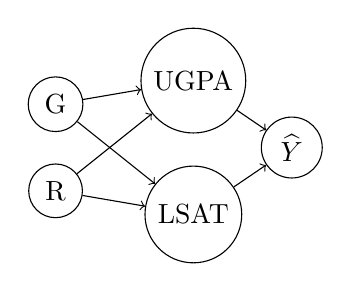
\begin{tikzpicture}
        \node (A1)  at (-1.75, -0.55) [circle, draw]{R};
        \node (A2)  at (-1.75, 0.55) [circle, draw]{G};
        \node (X1) at (0, 0.85) [circle, draw]{UGPA};
        \node (X2) at (0,-0.85) [circle,draw]{LSAT};
        \node (Y)  at (1.25, 0) [circle, draw]{$\widehat{Y}$};
        \draw[->] (A1) to (X1) {};
        \draw[->] (A1) to (X2) {};
        \draw[->] (A2) to (X1) {};
        \draw[->] (A2) to (X2) {};
        \draw[->] (X1) to (Y) {};
        % \draw[->] (X1) to (X2) {};
        \draw[->] (X2) to (Y) {};
    \end{tikzpicture}
\end{figure}
\end{minipage}
\begin{minipage}{.55\linewidth}
\begin{align*}
\mathcal{M} \, & 
\begin{cases}
    R & \leftarrow U_{R}\\
    G & \leftarrow U_G \\
    UGPA & \leftarrow b_U + \beta_1 \cdot R + \lambda_1 \cdot G + U_1, \ \\
    LSAT & \leftarrow  \exp\{b_L + \beta_2 \cdot R + \lambda_2 \cdot G + U_2\}, \\
\end{cases}
\end{align*}
\begin{align*}
    \widehat{Y} & = b(UGPA, LSAT) 
    % \\
    % & = \mathbbm{1}\{(0.6 \cdot UGPA + 0.4 \cdot LSAT) > \psi\}
\end{align*}
\end{minipage}
\caption{The auxiliary causal knowledge for Section~\ref{sec:Experiments.Real}. Let $R$ denote race, $G$ gender, \textit{LSAT} law school admissions test scores, \textit{UGPA} undergraduate grade-point average, and $\hat{Y}$ the admissions decision by $b()$.}
\label{fig:LawSchool}
% \vspace{-2ex}
\end{figure}
%

Let us now consider the law school admissions scenario popularized by \textcite[Figure 2]{Kusner2017CF}.
We use US data from the Law School Admission Council survey \parencite{Wightman1998_LawDataSource}, and recreate an admissions scenario for a top US law school. 
We consider as protected attributes an applicant's gender (\textit{G}, male/female), and race (\textit{R}, white/non-white). 
We add the ADM $b(UGPA, LSAT) = \hat{Y}$, which considers the applicant's undergraduate grade-point average (\textit{UGPA}) and law school admissions test scores (LSAT). 
If an applicant is successful, $\widehat{Y}=1$; otherwise $\widehat{Y}=0$. 
We summarize the scenario in Figure~\ref{fig:LawSchool}.
We define the ADM $b()$ using the median entry requirements for the top US law school to derive the cutoff $\psi$.\footnote{That being Yale University Law School; see \url{https://www.ilrg.com/rankings/law/index/1/asc/Accept}}
Formally, we define $b()$ as $\mathbbm{1}\{(0.6 \cdot UGPA + 0.4 \cdot LSAT) > \psi\}$.
The cutoff is the weighted sum of 60\%  in \textit{UGPA} (3.93 over 4.00), and 40\%  \textit{LSAT} (46.1 over 48), giving a total of 20.8; the maximum possible score given $b()$ is 22. 
The SCM $\mathcal{M}$ and DAG $\mathcal{G}$ follow \textcite{Kusner2017CF},
with $b_U$ and $b_L$ denoting the intercepts; $\beta_1$, $\beta_2$, $\lambda_1$, $\lambda_2$ the weights; and $U_1 \sim \mathcal{N}$ and $U_2 \sim \text{Poi}$ the probability distributions.

We study the behavior of $b()$ toward $G$ and $R$.
The dataset $\mathcal{D}$ contains $n=21790$ applicants, 43.8\% being female, 16.1\% being non-white, and 8.4\% being non-white-female.
%
Despite $b()$ being externally imposed by us for the purpose of illustrating the CST framework, under $b()$ only 0.8\% of the female applicants are successful compared to 1.5\% of the male applicants; similarly, only 0.2\% of the non-white applicants are successful compared to 2.2\% of the white applicants.
It is also the case when considering the intersectional group of non-white-females, with only 0.06\% of these applicants being admitted to law school based on $b()$ compared to the 2.25\% of white-female, non-white-male, and white-male successful applicants.
Notice that $b()$ is highly selective, with an acceptance rate of just 2.31\%, or 505 out of 21790 applicants considered.
Using DP as a fairness metric, $b()$ would still be considered unfair toward female, non-white, and non-white-female applicants.

\subsubsection{Single Discrimination}
\label{sec:Experiments.Real.Single}

%
\begin{table}[t]
\caption{Number (and \% w.r.t.~non-whites) of individual discrimination cases based on $R$ using Figure~\ref{fig:LawSchool}. Marked by * are the statistically significant cases.}
  \label{table:k-results_RACE}
  \centering
  \begin{tabular}{cccccc}
    \toprule
    Method & $k=15$ & $k=30$ & $k=50$ & $k=100$ & $k=250$\\
    \midrule
    CST w/o & 256 (7.3\%) & 309 (8.8\%) & 337 (9.6\%) & 400 (11.4\%)  & 503 (14.4\%) \\
     & 244* (6.9\%) & 301* (8.6\%) & 323* (9.2\%) & 391* (11.2\%)  & 494* (14.1\%) \\
     \midrule
    ST & 33 (0.9 \%) & 51 (1.5\%) & 61 (1.7\%) & 64 (1.8\%) & 78 (2.2\%) \\
    & 28* (0.8\%) & 28* (0.8\%) & 45* (1.3\%) & 47* (1.3\%) & 61 (1.7\%) \\
    \midrule
    CST w/ & 286 (8.2\%) & 309 (8.8\%) & 337 (9.6\%) & 400 (11.4\%)  & 503 (14.4\%)\\
    & 244* (6.9\%) & 301* (8.6\%) & 323* (9.2\%) & 391* (11.2\%)  & 494* (14.1\%) \\
    \midrule
    CF & 231 (6.6\%) & 231 (6.6\%) & 231 (6.6\%) &  231 (6.6\%) &  231 (6.6\%) \\
    & 190* (5.4\%) & 231* (6.6\%) & 231* (6.6\%) & 231* (6.6\%) & 231* (6.6\%) \\
    \bottomrule
  \end{tabular}
\end{table}
%

%
\begin{table}[t]
\caption{Number (and \% w.r.t.~females) of individual discrimination cases based on $G$ Figure~\ref{fig:LawSchool}. Marked by * are the statistically significant cases.}
  \label{table:k-results_GENDER}
  \centering
  \begin{tabular}{cccccc}
    \toprule
    Method & $k=15$ & $k=30$ & $k=50$ & $k=100$ & $k=250$\\
    \midrule
    CST w/o & 78 (0.8\%) & 120 (1.3\%) & 253 (2.7\%) & 296 (3.1\%)  & 493 (5.2\%) \\
     & 43* (0.5\%) & 88* (0.9\%) & 160* (1.7\%) & 221* (2.3\%)  & 341* (3.6\%) \\
     \midrule
    ST & 77 (0.8\%) & 101 (1.1\%) & 229 (2.4\%) & 258 (2.7\%) & 484 (5.1\%) \\
    & 57* (0.6\%) & 69* (0.7\%) & 111* (1.2\%) & 124* (1.3\%) & 366 (3.8\%) \\
    \midrule
    CST w/ & 99 (1.0\%) & 129 (1.4\%) & 267 (2.8\%) & 296 (3.1\%)  & 493 (5.2\%)\\
    & 54* (0.6\%) & 92* (0.9\%) & 160* (1.7\%) & 221* (2.3\%)  & 341* (3.6\%) \\
    \midrule
    CF & 56 (0.6\%) & 56 (0.6\%) & 56 (0.6\%) &  56 (0.6\%) &  56 (0.6\%) \\
    % & 20* (0.2\%) & 15* (0.2\%) & 30* (0.3\%) & 21* (0.2\%) & 32* (0.3\%) \\
    & 20* (0.2\%) & 15* (0.2\%) & 30* (0.3\%) & 21* (0.2\%) & 32* (0.3\%) \\
    \bottomrule
  \end{tabular}
\end{table}
%

Does $b()$ discriminate against non-white applicants? 
To answer this question using CST and CF, we generate the corresponding $\mathcal{D}^{CF}_R$ using Figure~\ref{fig:LawSchool} based in the intervention $do(R:=0)$, or \textit{what would have happened had all law school applicants been white?}
Similarly, does $b()$ discriminate against female applicants?
To answer this question using CST and CF, we generate the corresponding $\mathcal{D}^{CF}_G$ using Figure~\ref{fig:LawSchool} based in the intervention $do(G:=0)$, or \textit{what would have happened had all law school applicants been male?}
Both questions share the same $\mathcal{D}$.
Similar to Section~\ref{sec:Experiments.IllustrativeExample}, we use Definition~\ref{def:IndDisc} for detecting individual discrimination cases and Definition~\ref{def:CIs} for determining whether these cases are statistically significant.
Tables~\ref{table:k-results_RACE} and \ref{table:k-results_GENDER} show the results for all methods.
 
Tables~\ref{table:k-results_RACE} and \ref{table:k-results_GENDER} report similar patterns to those in Table~\ref{table:k-results}.
CST w/o detects a higher number of cases than ST; CST w/ detects a high number of cases than CF; and CST w/ detects a higher number than CST w/o. 
For all these patterns, though, the differences between the corresponding methods is smaller than those observed in Table~\ref{table:k-results}.
This is due to the composition of $\mathcal{D}$ and the nature of $b()$. 
Here, we work with a larger $\mathcal{D}$ (21790 versus 5000 applicants) and a more selective $b()$ (2.31\% versus 53.3\% acceptance rate).
CST w/o and CST w/ in Table~\ref{table:k-results_GENDER} converge already at larger neighborhood sizes, which does not occur in Table~\ref{table:k-results} (there is, though, a clear pattern that it occurs eventually as shown in Figure~\ref{fig:TwoCSTs_k_param}).
We also observe similar patterns once we account for statistical significance with CST w/o and CST w/ reaching the same number of cases in both tables for $k=250$.

%
\begin{figure}[t]
    \begin{subfigure}{.45\linewidth}
    \includegraphics[scale=0.45]{figures/R_all_delta_versus_k.png}
    \caption{}
     % \label{fig:a}
    \end{subfigure}
\hfill
    \begin{subfigure}{.45\linewidth}
    \includegraphics[scale=0.45]{figures/G_all_delta_versus_k.png}
    \caption{}
     % \label{fig:b}
    \end{subfigure}
\medskip
   \begin{subfigure}{.45\linewidth}
    \includegraphics[scale=0.45]{figures/R_all_nums_versus_k.png}
    \caption{}
     % \label{fig:c}
    \end{subfigure}
\hfill
    \begin{subfigure}{.45\linewidth}
    \includegraphics[scale=0.45]{figures/G_all_nums_versus_k.png}
    \caption{}
     % \label{fig:d}
    \end{subfigure}
\caption{Average $\Delta p$ and number of cases for race ($R$) and gender ($G$), respectively. We plot all and statistically significant (sig.) cases for each method.}
\label{fig:LawSchoolSingleDiscrimiantion_allmethods_k_param}
\end{figure}
%

Figure~\ref{fig:LawSchoolSingleDiscrimiantion_allmethods_k_param} supports Tables~\ref{table:k-results_RACE} and \ref{table:k-results_GENDER}, showing the average $\Delta p$ and the number of cases up to $k=500$ for all methods.\footnote{Due the size of $\mathcal{D}$, we run the methods for $k$ equals 1, 15, 30 and between 50-500 in increments of 10.} 
For the average $\Delta p$, as shown in sub-figures (a) and (b), it decreases as $k$ increases, with all methods seemingly converging to a single value.
%
% Notably, 
By observing that, as $k \rightarrow \infty$, the neighborhoods of the complainant and its counterfactual include all protected and unprotected instances, respectively, in $\mathcal{D}$, this value turns out to be the difference in DP: $P(\hat{Y}|A=1) - P(\hat{Y}|A=0)$ (cfr., footnote~\ref{foot:dp}) .
%
The average $\Delta p$ for significant cases is higher to, see ST in (a), or almost the same as, see CST w/ in (a), for all the cases.  
As $k$ increases, the control and tests groups constructed by ST, CST w/o, and CST w/ start considering new instances further away from the search centers and whatever detected initial deviation from $\tau$ dissipates slowly.
%
Similarly, as shown in sub-figures (c) and (d), the number of cases increases as $k$ increases except for CF which is independent of $k$ and its significant cases that are bounded by CF itself. 
We observe the CST versions converging, especially when accounting for statistical significance, while ST remains below both CST versions in (c) and mimics CST w/o in (d).
The number of significant cases is lower to ST in (c), or almost the same as both CST versions in (c) for all cases. 

The number of cases varies across the methods between Tables~\ref{table:k-results_RACE} and \ref{table:k-results_GENDER}. 
This is due to race and gender having different non-protected and protected search spaces.
The results are comparable, but represent separate tests for single discrimination.
Recall that non-whites represent 16.1\% while females represent 43.8\% of $\mathcal{D}$. 
It means that CST has access to a smaller search space when building the control groups for non-white complainants relative to female complainants.
Notably, in Table~\ref{table:k-results_RACE} statistically significant CF cases reach the 231 CF total cases within the $k$ values considered. 
This does not occur in Table~\ref{table:k-results_GENDER} in which the statistically significant CF cases slowly increase, though in a non-monotonically way, toward the 56 CF total cases.
Such oscillation, we believe, is due to the statistical estimator not yet reaching its asymptotic behavior.
These are, though, minor fluctuations as the number of statistically significant cases is around 0.2-0.3\%.\footnote{We use the CI \eqref{eq:CIs} from CST w/ though conditioned on CF discrimination occurring. We only detect 56 cases of CF discrimination (Table~\ref{table:k-results_GENDER}). As $k$ increases, we always look at these complainants.}
In Figure~\ref{fig:LawSchoolSingleDiscrimiantion_allmethods_k_param} we observe this non-monotonic increase for number of cases and decrease for the average $\Delta p$ of cases detected more clearly in the sub-figures (a) and (c) for race than for the sub-figures (b) and (d) for gender. 
The plots for gender are considerably less smooth than those for race. 
The composition of $\mathcal{D}$ clearly plays a role here as females represent 43.8\% and non-whites 16.1\% of the dataset, with the k-NN based methods varying more between iterations as they explore a much denser search space.

\subsubsection{Multidimensional Discrimination}
\label{sec:Experiments.Real.Multi}

We present the results for the forms of multidimensional discrimination, multiple and intersectional.
Given the focus on gender and race, the non-protected group amounts to the non-protected groups based on race and gender: i.e., white and male applicants.
As these two groups of applicants are not mutually exclusive, white-females and non-white-males are also part of the non-protected group.
This point is clearer when we consider the intersection of race and gender and focus on the protected group that is non-white-female applicants: the complementary of such group, meaning the non-protected group, includes white-female, non-white-male, and white-male applicants.

%
\begin{table}[t]
  \caption{Number (and \% w.r.t.~non-white-females) of multiple individual discrimination cases in Section~\ref{sec:Experiments.Real} for $R$ and $G$. Marked by * are the statistically significant cases.}
  \label{table:k-results_Multiple}
  \centering
  \begin{tabular}{cccccc}
    \toprule
    Method & $k=15$ & $k=30$ & $k=50$ & $k=100$ & $k=250$\\
    \midrule
    CST w/o & 8 (0.44\%) & 10 (0.55\%) & 20 (1.09\%) & 20 (1.09\%)  & 40 (2.18\%) \\
     & 4* (0.22\%) & 6* (0.33\%) & 11* (0.60\%) & 17* (0.93\%)  & 24* (1.31\%) \\
     \midrule
    ST & 5 (0.27\%) & 5 (0.27\%) & 12 (0.65\%) & 19 (1.04\%) & 24 (5.1\%) \\
    & 0* (0.0\%) & 0* (0.0\%) & 5* (0.27\%) & 5* (0.27\%)  & 15* (0.82\%) \\
    \midrule
    CST w/ & 9 (0.49\%) & 10 (0.55\%) & 21 (1.15\%) & 20 (1.09\%)  & 40 (2.18\%)\\
    & 4* (0.22\%) & 9* (0.49\%) & 11* (0.60\%) & 17* (0.93\%)  & 24* (1.31\%) \\
    \midrule
    CF & 5 (0.27\%) & 5 (0.27\%) & 5 (0.27\%) & 5 (0.27\%) & 5 (0.27\%) \\
    & 0* (0.0\%) & 3* (0.16\%) & 1* (0.05\%) & 1* (0.05\%) & 2* (0.11\%) \\
    \bottomrule
  \end{tabular}
\end{table}
%

%
\begin{table}[t]
  \caption{Number (and \% w.r.t.~non-white-females) of intersectional individual discrimination cases in Section~\ref{sec:Experiments.Real} for $R \times G$. Marked by * are the statistically significant cases.}
  \label{table:k-results_Intersectional}
  \centering
  \begin{tabular}{cccccc}
    \toprule
    Method & $k=15$ & $k=30$ & $k=50$ & $k=100$ & $k=250$\\
    \midrule
    CST w/o & 130 (7.1\%) & 138 (7.5\%) & 148 (8.1\%) & 160 (8.7\%)  & 199 (10.9\%) \\
    & 130* (7.1\%) & 138* (7.5\%) & 148* (8.1\%) & 160* (8.7\%)  & 199* (10.9\%) \\
     \midrule
    ST & 14 (0.8\%) & 14 (0.8\%) & 17 (0.9\%) & 24 (1.3\%) & 29 (1.6\%) \\
    & 14* (0.8\%) & 14* (0.8\%) & 13* (0.7\%) & 23* (1.3\%)  & 26* (1.4\%) \\
    \midrule
    CST w/ & 130 (7.1\%) & 138 (7.5\%) & 148 (8.1\%) & 160 (8.7\%)  & 199 (10.9\%) \\
    & 130* (7.1\%) & 138* (7.5\%) & 148* (8.1\%) & 160* (8.7\%)  & 199* (10.9\%) \\
    \midrule
    CF & 113 (6.2\%) & 113 (6.2\%) & 113 (6.2\%) & 113 (6.2\%) & 113 (6.2\%) \\
    & 113* (6.2\%) & 113* (6.2\%) & 113* (6.2\%) & 113* (6.2\%) & 113* (6.2\%) \\
    \bottomrule
  \end{tabular}
\end{table}
%

Following Definition~\ref{def:MultipleDisc}, we count as multiple discrimination based on race and gender when $\Delta p > \tau$ occurs separately for each of these protected attributes. 
Only those cases that are statistically significant for each protected attribute under CI \eqref{eq:CIs}---given the Bonferroni corrected $\alpha/2$---amount to statistically significant cases. 
We still rely on the generated $\mathcal{D}_R^{CF}$ and $\mathcal{D}_G^{CF}$ for the construction of the test groups and the original $\mathcal{D}$ for the construction of the control groups.
%
Does $b()$ discriminate against the none-white-female applicants as non-white \textit{and} as female applicants?
We present the results in Table~\ref{table:k-results_Multiple}. 
Figure~\ref{fig:LawSchoolMultiDiscrimination_allmethods_k_param}, as shown in sub-figures (a) and (c), further illustrates the results up to $k=500$. 
For the average $\Delta p$, we average those from cases detected separately under race and gender.

Following Definition~\ref{def:IntersectionaleDisc}, instead, we count intersectional discrimination based on race and gender when $\Delta p > \tau$ occurs for the intersection of these protected attributes. 
In practice, it means constructing the new protected attribute $R \times G$; updating $\mathcal{D}$ into $\mathcal{D}'$, such that $R \times G \in \mathcal{D}'$; and generating $\mathcal{D}'^{CF}$ given Figure~\ref{fig:LawSchool} under $do(R \times G := 0)$.
It implies a single discrimination run but under the ``new'' single attribute $R \times G$, representing the intersection of $R$ and $G$. 
Cases are statistically significant under CI \eqref{eq:CIs} based on $R \times G$.
Formally, in Figure~\ref{fig:LawSchool} we merge the $R$ and $G$ nodes into the single $R \times G$ in $\mathcal{G}$ node and do the same for the corresponding equations in $\mathcal{M}$ by interacting the dummy variables for $R$ and $G$ and re-estimating the regression weights \parencite{Wooldridge2015IntroductoryEconometrics}.
%
Does $b()$ discriminate against the none-white-female applicants?
We present the results in Table~\ref{table:k-results_Intersectional}.
Figure~\ref{fig:LawSchoolMultiDiscrimination_allmethods_k_param}, as shown in sub-figures (b) and (d), further illustrates the results up to $k=500$.

In Tables~\ref{table:k-results_Multiple} and \ref{table:k-results_Intersectional}, the three methods show similar patterns between them.
CST w/o detects more cases relative to ST (including statistically significant cases); CST w/ detects more cases than CF (including statistically significant cases); and the two CST versions converge once statistical significance is considered.
The same line of reasoning used before still applies here for understanding how CST, ST, and CF relate to each other.
The difference is that the protected group and, in turn, the non-protected group are defined by more than one protected attribute.
What is interesting in Table~\ref{table:k-results_Multiple} is that CST w/o and CST w/ converge early on for all cases, not just for those cases that are statistically significant.
We suspect these are cases that are clearly discriminatory under both race and gender, making them likely to be detected by multiple and intersectional discrimination testing.
All cases in Table~\ref{table:k-results_Intersectional} are also statistically significant for all methods.
It is due to $R \times G=1$ representing the most un-favored protected group from the combination of $R$ and $G$, which results in larger $\Delta p$'s and a complete convergence of all and statistically significant cases for all methods relative to multiple discrimination. 
Compare, e.g.,~(a) versus (b) and (c) versus (d) in Figure~\ref{fig:LawSchoolMultiDiscrimination_allmethods_k_param}. 
We discuss the last point in the next section.  

\subsubsection{On Multiple and Intersectional Discrimination}
\label{sec:Experiments.Real.Multiple_vs_Intersectional}

The results from the previous section support claims by legal scholars on the risk of not recognizing intersectional discrimination under non-discrimination law.
These claims, to the best of our knowledge, date back to \textcite{Crenshaw1989_DemarginalizingTheIntersection} and have become prominent again with the ongoing discussion around algorithmic discrimination \parencite{Xenidis2020_TunningEULaw}.
We suspect that, since multiple and intersectional discrimination share the protected group and the non-protected groups, there is a tendency to dismiss the latter as a special case of the former.
An in-depth legal discussion on the tension between multiple and intersectional discrimination is beyond this paper, but Tables~\ref{table:k-results_Multiple} and \ref{table:k-results_Intersectional} support the calls by these researchers to treat intersectional discrimination separate from multiple discrimination.

%
\begin{figure}[t]
    \begin{subfigure}{.45\linewidth}
    \includegraphics[scale=0.45]{figures/Multi_all_deltas_versus_k.png}
    \caption{}
    \end{subfigure}
\hfill
    \begin{subfigure}{.45\linewidth}
    \includegraphics[scale=0.45]{figures/Inter_all_deltas_versus_k.png}
    \caption{}
    \end{subfigure}
    \medskip
    \begin{subfigure}{.45\linewidth}
    \includegraphics[scale=0.45]{figures/Multi_all_nums_versus_k.png}
    \caption{}
     % \label{fig:c}
    \end{subfigure}
\hfill
    \begin{subfigure}{.45\linewidth}
    \includegraphics[scale=0.45]{figures/Inter_all_nums_versus_k.png}
    \caption{}
     % \label{fig:d}
    \end{subfigure}
\caption{Avg. $\Delta p$ and number of cases for multiple (left) and intersectional (right) discrimination on $R$ and $G$. We plot all and statistically significant (sig.) cases for all methods.}
\label{fig:LawSchoolMultiDiscrimination_allmethods_k_param}
\end{figure}
%

We acknowledge that, from a modeling perspective, a difference between Tables~\ref{table:k-results_Multiple} and \ref{table:k-results_Intersectional} is expected since we implement different procedures.
Under multiple discrimination we look at the intersection of two separate single discrimination testing runs, while under intersectional discrimination we look at a single discrimination run representing the intersection. 
%
The claims by legal scholars like \textcite{Crenshaw1989_DemarginalizingTheIntersection, Xenidis2020_TunningEULaw}, however, were not as apparent to us, meaning, in principle, we had no reason to expect a higher number of cases for intersectional discrimination over multiple discrimination.
%
In fact, from a probability theory perspective (read, the conjunction rule), if we had to choose a difference between the Tables~\ref{table:k-results_Multiple} and \ref{table:k-results_Intersectional}, we would have guessed the opposite, with multiple discrimination acting as an upper limit to intersectional discrimination.
Given these results, we now would add that such expectation holds from a modeling perspective if we agree that the intersection of $G$ and $R$ is not its own category. Let us discuss further.

The two modeling procedures allow to represent the case in which $R \times G$ is its own category (intersectional) and in which is just the conjunction of $R$ and $G$ (multiple).
This distinction, with legal origins as already argued \parencite{Crenshaw1989_DemarginalizingTheIntersection}, in fact materializes through the counterfactual representation of each complainant under these two discrimination testing procedures.
Under multiple discrimination, we still rely on $\mathcal{D}_R^{CF}$ and $\mathcal{D}_G^{CF}$ for running the methods separately on $R$ and $G$. 
We look at male and non-white conterfactuals separately. 
Although together they cover all the non-protected groups, they do not do so simultaneously: the complainant under this procedure would have been male or non-white, but not female-non-white.
%
Under intersectional discrimination, instead, we rely on updated factual and counterfactual datasets based on a ``new'' protected attribute $R \times G$. 
The counterfactual for a given compliant implies simultaneously the possibilities of white-male, white-female, and non-white-male, which introduces more randomness.
 
In Figure~\ref{fig:LawSchool}, arguably, the worst-off sub-group between $R$ and $G$ is the group of non-white-female applicants.
% Following the reasoning used in the previous paragraph,
The logic here is that non-white males, meaning $R=1$ and $G=0$, can always resort to their gender and white females, meaning $R=0$ and $G=1$, can always resort to their race.
Instead, non-white females have no single group within the space of $R \times G$ to resort to.
When we test for multiple discrimination we allow for these movements to occur by looking at $R$ and $G$ separately. 
This is because, by not intersecting $R$ and $G$, we do not consider the fact that the group at the intersection never has the choice to resort to a non-protected group. 
This lack of choice is what we represent when we test for intersectional discrimination by looking at $R \times G$ only.
%
The modeling problem for these forms of multidimensional discrimination requires further research with the goal of formalizing the role of the intersection and how it influences the control and test search spaces while taking into account the legal considerations discussed.

Back to Tables~\ref{table:k-results_Multiple} and \ref{table:k-results_Intersectional}, we argue that the observed difference comes from one protected attribute having a stronger influence than the other on the non-protected attributes. 
If that is the case, then testing separately for $R$ and $G$ should show individuals that are discriminated only by one of the protected attributes, which dismisses the multiple discrimination claim.
%
Table~\ref{table:MultivsInter} supports this argument. 
%
Notably, it is for this reason that lawyers discourage multiple discrimination claims and suggest that the complainant focuses on the most dominant protected attribute \parencite{Xenidis2020_TunningEULaw}.

In Table~\ref{table:MultivsInter}, given the results from the previous section, we focus on CST w/o for $k=15$ and look at individual discrimination cases detected as both multiple and intersectional discrimination.
We report the average $p_c$ and $p_t$ for $R$, $G$, and $R \times G$.
% We note that 
All multiple cases are included in the intersectional cases detected by CST w/o.
The first row shows these multiple discrimination cases. We observe that the average $p_c$ is greater than the average $p_t$, and thus the average $\Delta p > \tau$, for $R$, $G$, and $R \times G$. 
These are individual cases that suffer the negative effects of $R$ and $G$, separately and simultaneously, when applying to law school under $b()$.
The second row, instead, shows the intersectional cases only. 
For comparison, we provide the average $p_c$ and $p_t$ for these individuals' single discrimination tests for $R$ and $G$.
We observe that, on average, $R$ is the dominant protected attribute with a considerable difference in the proportion of negative outcomes between the control and test groups. 
This is not the case for $G$ where the average difference is negligible. 
Indeed, for these individuals, by looking at each protected attribute separately, we lose the multiple discrimination case.
In doing so, we also lose focus on what occurs at the intersection of $R \times G$.
The results in Table~\ref{table:MultivsInter} capture this lack of movement between protected and non-protected statuses experienced by those individuals at the bottom of the intersection of $R$ and $G$.

%
\begin{table}[t]
\caption{Avg. $p_c$ and $p_t$ for the ctr's and tst's groups of CST w/o for $k=15$.}
  \label{table:MultivsInter}
  \centering
  \begin{tabular}{ccccccc}
    \toprule
    & \multicolumn{6}{c}{Average}\\
    & $G$'s $p_c$ & $G$'s $p_t$ & $R$'s $p_c$ & $R$'s $p_t$ & $R \times G$'s $p_c$ & $R \times G$'s $p_t$\\
    \midrule
    Multi. and inter. & 0.59 & 0.33 & 0.51 & 0.00 & 0.66 & 0.00 \\
    Inter. only & 0.96 & 0.94 & 0.93 & 0.23 & 0.93 & 0.01 \\
    \bottomrule
  \end{tabular}
\end{table}
%

%
% EOS
%

% This file was created by matlab2tikz.
%
%The latest updates can be retrieved from
%  http://www.mathworks.com/matlabcentral/fileexchange/22022-matlab2tikz-matlab2tikz
%where you can also make suggestions and rate matlab2tikz.
%
\definecolor{mycolor1}{rgb}{0.21569,0.54902,0.72157}%
\definecolor{mycolor2}{rgb}{0.80784,0.16863,0.12157}%
%
\begin{tikzpicture}

\begin{axis}[%
width=0.898in,
height=1.5in,%3.603in,
at={(0.766in,0.486in)},
scale only axis,
xmin=0,
xmax=10,
ymin=0,
ymax=0.8,
xlabel= \phantom{$z$},
ylabel=$p(g_{z^*}|Y)$,
ylabel near ticks,
title={Linearization-based\\ approach},
title style={align=left}, 
axis background/.style={fill=white},
axis x line*=bottom,
axis y line*=left,
legend style={legend cell align=left, align=left, draw=white!15!black}
]
\addplot[ybar interval, fill=mycolor1, fill opacity=0.4, draw=mycolor1, area legend] table[row sep=crcr] {%
x	y\\
3.36	0.0144927536231884\\
3.429	0.0289855072463768\\
3.498	0.0869565217391305\\
3.567	0.217391304347825\\
3.636	0.391304347826087\\
3.705	0.565217391304348\\
3.774	0.449275362318841\\
3.843	0.405797101449276\\
3.912	0.666666666666667\\
3.981	0.420289855072464\\
4.05	0.478260869565218\\
4.119	0.289855072463768\\
4.188	0.289855072463768\\
4.257	0.347826086956522\\
4.326	0.246376811594203\\
4.395	0.304347826086953\\
4.464	0.20289855072464\\
4.533	0.217391304347823\\
4.602	0.246376811594203\\
4.671	0.289855072463768\\
4.74	0.246376811594203\\
4.809	0.188405797101449\\
4.878	0.231884057971015\\
4.947	0.27536231884058\\
5.016	0.391304347826087\\
5.085	0.246376811594203\\
5.154	0.27536231884058\\
5.223	0.217391304347826\\
5.292	0.347826086956518\\
5.361	0.231884057971018\\
5.43	0.2463768115942\\
5.499	0.260869565217395\\
5.568	0.275362318840576\\
5.637	0.289855072463772\\
5.706	0.304347826086953\\
5.775	0.289855072463772\\
5.844	0.362318840579706\\
5.913	0.289855072463768\\
5.982	0.463768115942029\\
6.051	0.420289855072464\\
6.12	0.492753623188406\\
6.189	0.463768115942029\\
6.258	0.463768115942029\\
6.327	0.420289855072459\\
6.396	0.246376811594206\\
6.465	0.202898550724635\\
6.534	0.0869565217391316\\
6.603	0.0579710144927529\\
6.672	0.0289855072463772\\
6.741	0.0144927536231882\\
6.81	0.0144927536231882\\
};
%\addlegendentry{ground truth}

\addplot [color=mycolor2, line width=2.0pt]
  table[row sep=crcr]{%
0	0.00495647934021539\\
0.01	0.00503120737369003\\
0.02	0.00510691052511148\\
0.03	0.00518359894024572\\
0.04	0.00526128282899922\\
0.05	0.00533997246516116\\
0.06	0.00541967818613227\\
0.07	0.00550041039264009\\
0.08	0.00558217954844049\\
0.09	0.00566499618000535\\
0.1	0.00574887087619621\\
0.11	0.00583381428792371\\
0.12	0.00591983712779276\\
0.13	0.00600695016973323\\
0.14	0.006095164248616\\
0.15	0.00618449025985429\\
0.16	0.00627493915898998\\
0.17	0.00636652196126503\\
0.18	0.0064592497411776\\
0.19	0.0065531336320228\\
0.2	0.00664818482541805\\
0.21	0.0067444145708128\\
0.22	0.0068418341749824\\
0.23	0.00694045500150619\\
0.24	0.00704028847022945\\
0.25	0.00714134605670927\\
0.26	0.00724363929164408\\
0.27	0.00734717976028668\\
0.28	0.00745197910184082\\
0.29	0.00755804900884096\\
0.3	0.00766540122651533\\
0.31	0.00777404755213196\\
0.32	0.00788399983432761\\
0.33	0.00799526997241961\\
0.34	0.00810786991570027\\
0.35	0.00822181166271396\\
0.36	0.00833710726051655\\
0.37	0.00845376880391716\\
0.38	0.00857180843470236\\
0.39	0.00869123834084212\\
0.4	0.00881207075567811\\
0.41	0.00893431795709363\\
0.42	0.00905799226666551\\
0.43	0.00918310604879767\\
0.44	0.00930967170983618\\
0.45	0.00943770169716588\\
0.46	0.00956720849828854\\
0.47	0.00969820463988202\\
0.48	0.00983070268684103\\
0.49	0.00996471524129867\\
0.5	0.0101002549416293\\
0.51	0.0102373344614323\\
0.52	0.0103759665084967\\
0.53	0.0105161638237465\\
0.54	0.0106579391801673\\
0.55	0.0108013053817126\\
0.56	0.010946275262192\\
0.57	0.0110928616841387\\
0.58	0.0112410775376588\\
0.59	0.0113909357392594\\
0.6	0.0115424492306589\\
0.61	0.0116956309775763\\
0.62	0.0118504939685016\\
0.63	0.0120070512134457\\
0.64	0.0121653157426715\\
0.65	0.012325300605404\\
0.66	0.012487018868522\\
0.67	0.0126504836152284\\
0.68	0.0128157079437017\\
0.69	0.0129827049657272\\
0.7	0.0131514878053083\\
0.71	0.0133220695972577\\
0.72	0.0134944634857689\\
0.73	0.0136686826229678\\
0.74	0.0138447401674437\\
0.75	0.0140226492827617\\
0.76	0.0142024231359536\\
0.77	0.0143840748959895\\
0.78	0.0145676177322305\\
0.79	0.0147530648128596\\
0.8	0.0149404293032943\\
0.81	0.0151297243645786\\
0.82	0.0153209631517556\\
0.83	0.0155141588122201\\
0.84	0.0157093244840515\\
0.85	0.0159064732943274\\
0.86	0.0161056183574168\\
0.87	0.016306772773255\\
0.88	0.0165099496255975\\
0.89	0.0167151619802561\\
0.9	0.0169224228833143\\
0.91	0.017131745359324\\
0.92	0.0173431424094836\\
0.93	0.0175566270097958\\
0.94	0.0177722121092072\\
0.95	0.0179899106277294\\
0.96	0.0182097354545399\\
0.97	0.018431699446066\\
0.98	0.0186558154240489\\
0.99	0.0188820961735898\\
1	0.0191105544411779\\
1.01	0.0193412029326999\\
1.02	0.0195740543114314\\
1.03	0.0198091211960107\\
1.04	0.0200464161583947\\
1.05	0.0202859517217969\\
1.06	0.0205277403586084\\
1.07	0.0207717944883015\\
1.08	0.0210181264753159\\
1.09	0.0212667486269282\\
1.1	0.0215176731911045\\
1.11	0.0217709123543368\\
1.12	0.0220264782394623\\
1.13	0.0222843829034672\\
1.14	0.0225446383352741\\
1.15	0.0228072564535138\\
1.16	0.0230722491042814\\
1.17	0.0233396280588773\\
1.18	0.0236094050115328\\
1.19	0.0238815915771207\\
1.2	0.0241561992888519\\
1.21	0.0244332395959568\\
1.22	0.0247127238613533\\
1.23	0.0249946633592999\\
1.24	0.0252790692730363\\
1.25	0.0255659526924097\\
1.26	0.0258553246114888\\
1.27	0.026147195926164\\
1.28	0.0264415774317359\\
1.29	0.0267384798204914\\
1.3	0.0270379136792673\\
1.31	0.0273398894870028\\
1.32	0.0276444176122807\\
1.33	0.0279515083108568\\
1.34	0.0282611717231799\\
1.35	0.0285734178718998\\
1.36	0.0288882566593667\\
1.37	0.0292056978651199\\
1.38	0.0295257511433677\\
1.39	0.0298484260204579\\
1.4	0.0301737318923396\\
1.41	0.0305016780220172\\
1.42	0.0308322735369956\\
1.43	0.0311655274267189\\
1.44	0.0315014485400004\\
1.45	0.0318400455824475\\
1.46	0.0321813271138789\\
1.47	0.032525301545736\\
1.48	0.0328719771384891\\
1.49	0.0332213619990379\\
1.5	0.0335734640781073\\
1.51	0.0339282911676388\\
1.52	0.034285850898178\\
1.53	0.0346461507362581\\
1.54	0.0350091979817809\\
1.55	0.0353749997653947\\
1.56	0.0357435630458696\\
1.57	0.0361148946074719\\
1.58	0.0364890010573359\\
1.59	0.0368658888228363\\
1.6	0.0372455641489584\\
1.61	0.0376280330956701\\
1.62	0.0380133015352924\\
1.63	0.0384013751498731\\
1.64	0.0387922594285599\\
1.65	0.0391859596649766\\
1.66	0.0395824809546015\\
1.67	0.0399818281921483\\
1.68	0.040384006068951\\
1.69	0.0407890190703521\\
1.7	0.0411968714730958\\
1.71	0.0416075673427256\\
1.72	0.0420211105309874\\
1.73	0.0424375046732393\\
1.74	0.0428567531858665\\
1.75	0.0432788592637046\\
1.76	0.0437038258774694\\
1.77	0.0441316557711956\\
1.78	0.0445623514596833\\
1.79	0.0449959152259539\\
1.8	0.0454323491187165\\
1.81	0.0458716549498434\\
1.82	0.0463138342918566\\
1.83	0.0467588884754263\\
1.84	0.047206818586881\\
1.85	0.0476576254657295\\
1.86	0.0481113097021966\\
1.87	0.0485678716347722\\
1.88	0.0490273113477746\\
1.89	0.0494896286689283\\
1.9	0.0499548231669573\\
1.91	0.0504228941491942\\
1.92	0.0508938406592059\\
1.93	0.0513676614744362\\
1.94	0.0518443551038658\\
1.95	0.0523239197856913\\
1.96	0.0528063534850216\\
1.97	0.0532916538915952\\
1.98	0.0537798184175165\\
1.99	0.0542708441950129\\
2	0.0547647280742127\\
2.01	0.0552614666209458\\
2.02	0.0557610561145651\\
2.03	0.0562634925457924\\
2.04	0.0567687716145866\\
2.05	0.0572768887280368\\
2.06	0.0577878389982796\\
2.07	0.0583016172404419\\
2.08	0.0588182179706094\\
2.09	0.0593376354038221\\
2.1	0.0598598634520962\\
2.11	0.0603848957224738\\
2.12	0.0609127255151013\\
2.13	0.0614433458213363\\
2.14	0.0619767493218837\\
2.15	0.0625129283849627\\
2.16	0.063051875064503\\
2.17	0.0635935810983738\\
2.18	0.0641380379066434\\
2.19	0.0646852365898719\\
2.2	0.0652351679274361\\
2.21	0.0657878223758891\\
2.22	0.0663431900673527\\
2.23	0.0669012608079454\\
2.24	0.0674620240762456\\
2.25	0.0680254690217902\\
2.26	0.06859158446361\\
2.27	0.0691603588888017\\
2.28	0.0697317804511384\\
2.29	0.0703058369697168\\
2.3	0.070882515927644\\
2.31	0.0714618044707637\\
2.32	0.0720436894064212\\
2.33	0.0726281572022699\\
2.34	0.0732151939851174\\
2.35	0.0738047855398146\\
2.36	0.0743969173081847\\
2.37	0.0749915743879969\\
2.38	0.0755887415319811\\
2.39	0.0761884031468874\\
2.4	0.0767905432925892\\
2.41	0.0773951456812309\\
2.42	0.0780021936764202\\
2.43	0.0786116702924671\\
2.44	0.0792235581936674\\
2.45	0.079837839693634\\
2.46	0.0804544967546748\\
2.47	0.0810735109872175\\
2.48	0.0816948636492834\\
2.49	0.0823185356460092\\
2.5	0.0829445075292169\\
2.51	0.0835727594970344\\
2.52	0.084203271393565\\
2.53	0.0848360227086074\\
2.54	0.0854709925774259\\
2.55	0.0861081597805728\\
2.56	0.0867475027437606\\
2.57	0.0873889995377879\\
2.58	0.0880326278785163\\
2.59	0.0886783651269002\\
2.6	0.0893261882890704\\
2.61	0.0899760740164704\\
2.62	0.0906279986060465\\
2.63	0.0912819380004926\\
2.64	0.0919378677885496\\
2.65	0.0925957632053583\\
2.66	0.0932555991328697\\
2.67	0.0939173501003085\\
2.68	0.0945809902846947\\
2.69	0.0952464935114191\\
2.7	0.0959138332548775\\
2.71	0.0965829826391593\\
2.72	0.0972539144387952\\
2.73	0.0979266010795609\\
2.74	0.0986010146393384\\
2.75	0.0992771268490357\\
2.76	0.0999549090935642\\
2.77	0.100634332412874\\
2.78	0.101315367503047\\
2.79	0.101997984717452\\
2.8	0.102682154067954\\
2.81	0.103367845226185\\
2.82	0.104055027524874\\
2.83	0.104743669959238\\
2.84	0.105433741188425\\
2.85	0.106125209537028\\
2.86	0.106818042996652\\
2.87	0.107512209227537\\
2.88	0.108207675560252\\
2.89	0.108904408997439\\
2.9	0.109602376215622\\
2.91	0.110301543567076\\
2.92	0.111001877081754\\
2.93	0.111703342469276\\
2.94	0.112405905120979\\
2.95	0.113109530112027\\
2.96	0.113814182203577\\
2.97	0.114519825845015\\
2.98	0.115226425176241\\
2.99	0.115933944030024\\
3	0.116642345934409\\
3.01	0.117351594115192\\
3.02	0.118061651498449\\
3.03	0.118772480713129\\
3.04	0.119484044093701\\
3.05	0.120196303682873\\
3.06	0.120909221234355\\
3.07	0.121622758215693\\
3.08	0.122336875811159\\
3.09	0.123051534924699\\
3.1	0.123766696182943\\
3.11	0.124482319938267\\
3.12	0.125198366271925\\
3.13	0.12591479499723\\
3.14	0.126631565662796\\
3.15	0.127348637555838\\
3.16	0.128065969705534\\
3.17	0.128783520886434\\
3.18	0.129501249621939\\
3.19	0.130219114187826\\
3.2	0.130937072615837\\
3.21	0.131655082697321\\
3.22	0.132373101986931\\
3.23	0.133091087806378\\
3.24	0.133808997248241\\
3.25	0.13452678717983\\
3.26	0.135244414247106\\
3.27	0.135961834878651\\
3.28	0.136679005289694\\
3.29	0.137395881486191\\
3.3	0.138112419268956\\
3.31	0.138828574237848\\
3.32	0.139544301796001\\
3.33	0.140259557154114\\
3.34	0.14097429533479\\
3.35	0.141688471176923\\
3.36	0.142402039340136\\
3.37	0.143114954309265\\
3.38	0.143827170398901\\
3.39	0.144538641757969\\
3.4	0.145249322374359\\
3.41	0.145959166079606\\
3.42	0.146668126553618\\
3.43	0.147376157329438\\
3.44	0.148083211798065\\
3.45	0.148789243213316\\
3.46	0.149494204696722\\
3.47	0.150198049242482\\
3.48	0.150900729722448\\
3.49	0.151602198891158\\
3.5	0.152302409390905\\
3.51	0.153001313756856\\
3.52	0.153698864422194\\
3.53	0.154395013723319\\
3.54	0.155089713905069\\
3.55	0.155782917125992\\
3.56	0.156474575463644\\
3.57	0.157164640919932\\
3.58	0.157853065426486\\
3.59	0.158539800850068\\
3.6	0.15922479899801\\
3.61	0.159908011623694\\
3.62	0.160589390432051\\
3.63	0.161268887085104\\
3.64	0.16194645320753\\
3.65	0.16262204039226\\
3.66	0.163295600206099\\
3.67	0.163967084195381\\
3.68	0.164636443891645\\
3.69	0.165303630817341\\
3.7	0.165968596491557\\
3.71	0.166631292435772\\
3.72	0.167291670179631\\
3.73	0.167949681266742\\
3.74	0.168605277260496\\
3.75	0.169258409749901\\
3.76	0.169909030355445\\
3.77	0.170557090734967\\
3.78	0.171202542589549\\
3.79	0.171845337669428\\
3.8	0.17248542777992\\
3.81	0.173122764787353\\
3.82	0.173757300625023\\
3.83	0.174388987299154\\
3.84	0.175017776894874\\
3.85	0.1756436215822\\
3.86	0.176266473622029\\
3.87	0.176886285372142\\
3.88	0.177503009293208\\
3.89	0.178116597954805\\
3.9	0.178727004041434\\
3.91	0.179334180358544\\
3.92	0.179938079838555\\
3.93	0.180538655546892\\
3.94	0.181135860688006\\
3.95	0.181729648611403\\
3.96	0.182319972817676\\
3.97	0.182906786964519\\
3.98	0.183490044872755\\
3.99	0.184069700532347\\
4	0.184645708108407\\
4.01	0.185218021947199\\
4.02	0.185786596582135\\
4.03	0.186351386739756\\
4.04	0.186912347345709\\
4.05	0.187469433530713\\
4.06	0.188022600636505\\
4.07	0.188571804221778\\
4.08	0.189117000068111\\
4.09	0.189658144185865\\
4.1	0.190195192820082\\
4.11	0.190728102456354\\
4.12	0.191256829826677\\
4.13	0.191781331915283\\
4.14	0.192301565964453\\
4.15	0.192817489480306\\
4.16	0.193329060238567\\
4.17	0.193836236290307\\
4.18	0.194338975967659\\
4.19	0.19483723788951\\
4.2	0.195330980967159\\
4.21	0.195820164409952\\
4.22	0.196304747730887\\
4.23	0.196784690752181\\
4.24	0.197259953610816\\
4.25	0.197730496764038\\
4.26	0.198196280994839\\
4.27	0.198657267417387\\
4.28	0.19911341748243\\
4.29	0.199564692982658\\
4.3	0.200011056058033\\
4.31	0.200452469201067\\
4.32	0.200888895262076\\
4.33	0.201320297454377\\
4.34	0.201746639359454\\
4.35	0.202167884932071\\
4.36	0.202583998505353\\
4.37	0.202994944795806\\
4.38	0.203400688908302\\
4.39	0.203801196341013\\
4.4	0.204196432990295\\
4.41	0.204586365155525\\
4.42	0.204970959543887\\
4.43	0.205350183275104\\
4.44	0.205724003886121\\
4.45	0.206092389335735\\
4.46	0.206455308009166\\
4.47	0.206812728722581\\
4.48	0.207164620727553\\
4.49	0.207510953715471\\
4.5	0.207851697821886\\
4.51	0.208186823630804\\
4.52	0.208516302178914\\
4.53	0.208840104959761\\
4.54	0.209158203927852\\
4.55	0.209470571502708\\
4.56	0.209777180572843\\
4.57	0.210078004499687\\
4.58	0.210373017121445\\
4.59	0.210662192756884\\
4.6	0.21094550620906\\
4.61	0.211222932768978\\
4.62	0.211494448219179\\
4.63	0.211760028837266\\
4.64	0.212019651399358\\
4.65	0.212273293183472\\
4.66	0.212520931972839\\
4.67	0.212762546059146\\
4.68	0.212998114245707\\
4.69	0.213227615850562\\
4.7	0.213451030709505\\
4.71	0.213668339179034\\
4.72	0.21387952213923\\
4.73	0.214084560996561\\
4.74	0.214283437686611\\
4.75	0.214476134676732\\
4.76	0.214662634968617\\
4.77	0.214842922100803\\
4.78	0.215016980151093\\
4.79	0.215184793738895\\
4.8	0.21534634802749\\
4.81	0.21550162872622\\
4.82	0.215650622092589\\
4.83	0.215793314934298\\
4.84	0.215929694611184\\
4.85	0.216059749037091\\
4.86	0.216183466681654\\
4.87	0.216300836572001\\
4.88	0.21641184829438\\
4.89	0.21651649199569\\
4.9	0.216614758384949\\
4.91	0.21670663873466\\
4.92	0.216792124882109\\
4.93	0.21687120923057\\
4.94	0.216943884750432\\
4.95	0.21701014498024\\
4.96	0.217069984027651\\
4.97	0.21712339657031\\
4.98	0.217170377856636\\
4.99	0.217210923706529\\
5	0.21724503051199\\
5.01	0.217272695237652\\
5.02	0.217293915421236\\
5.03	0.217308689173911\\
5.04	0.217317015180578\\
5.05	0.217318892700066\\
5.06	0.217314321565234\\
5.07	0.217303302183007\\
5.08	0.217285835534308\\
5.09	0.217261923173913\\
5.1	0.217231567230225\\
5.11	0.217194770404953\\
5.12	0.217151535972715\\
5.13	0.217101867780549\\
5.14	0.217045770247346\\
5.15	0.216983248363191\\
5.16	0.216914307688628\\
5.17	0.21683895435383\\
5.18	0.216757195057696\\
5.19	0.216669037066854\\
5.2	0.216574488214588\\
5.21	0.216473556899676\\
5.22	0.216366252085147\\
5.23	0.216252583296955\\
5.24	0.216132560622568\\
5.25	0.216006194709479\\
5.26	0.215873496763628\\
5.27	0.215734478547749\\
5.28	0.21558915237963\\
5.29	0.215437531130296\\
5.3	0.215279628222107\\
5.31	0.215115457626779\\
5.32	0.214945033863324\\
5.33	0.21476837199591\\
5.34	0.214585487631638\\
5.35	0.21439639691825\\
5.36	0.21420111654175\\
5.37	0.213999663723949\\
5.38	0.213792056219935\\
5.39	0.213578312315465\\
5.4	0.213358450824282\\
5.41	0.213132491085352\\
5.42	0.212900452960033\\
5.43	0.212662356829162\\
5.44	0.212418223590075\\
5.45	0.212168074653546\\
5.46	0.211911931940665\\
5.47	0.211649817879627\\
5.48	0.211381755402469\\
5.49	0.21110776794172\\
5.5	0.210827879426989\\
5.51	0.210542114281486\\
5.52	0.210250497418463\\
5.53	0.209953054237604\\
5.54	0.209649810621332\\
5.55	0.209340792931057\\
5.56	0.209026028003361\\
5.57	0.208705543146111\\
5.58	0.208379366134512\\
5.59	0.2080475252071\\
5.6	0.207710049061664\\
5.61	0.207366966851112\\
5.62	0.207018308179279\\
5.63	0.206664103096667\\
5.64	0.206304382096132\\
5.65	0.205939176108512\\
5.66	0.205568516498194\\
5.67	0.20519243505863\\
5.68	0.204810964007791\\
5.69	0.204424135983574\\
5.7	0.204031984039149\\
5.71	0.203634541638252\\
5.72	0.203231842650435\\
5.73	0.202823921346256\\
5.74	0.202410812392424\\
5.75	0.201992550846891\\
5.76	0.201569172153899\\
5.77	0.201140712138983\\
5.78	0.200707207003916\\
5.79	0.200268693321625\\
5.8	0.199825208031051\\
5.81	0.199376788431969\\
5.82	0.198923472179769\\
5.83	0.198465297280192\\
5.84	0.198002302084028\\
5.85	0.197534525281773\\
5.86	0.197062005898254\\
5.87	0.196584783287207\\
5.88	0.196102897125829\\
5.89	0.195616387409288\\
5.9	0.195125294445206\\
5.91	0.1946296588481\\
5.92	0.194129521533804\\
5.93	0.193624923713846\\
5.94	0.193115906889808\\
5.95	0.192602512847652\\
5.96	0.192084783652017\\
5.97	0.191562761640493\\
5.98	0.19103648941787\\
5.99	0.19050600985036\\
6	0.189971366059799\\
6.01	0.189432601417827\\
6.02	0.188889759540044\\
6.03	0.188342884280149\\
6.04	0.187792019724062\\
6.05	0.187237210184025\\
6.06	0.186678500192687\\
6.07	0.186115934497179\\
6.08	0.185549558053167\\
6.09	0.184979416018895\\
6.1	0.184405553749221\\
6.11	0.183828016789635\\
6.12	0.183246850870269\\
6.13	0.182662101899903\\
6.14	0.182073815959955\\
6.15	0.181482039298473\\
6.16	0.180886818324118\\
6.17	0.18028819960014\\
6.18	0.179686229838354\\
6.19	0.179080955893116\\
6.2	0.17847242475529\\
6.21	0.177860683546225\\
6.22	0.177245779511726\\
6.23	0.176627760016027\\
6.24	0.176006672535775\\
6.25	0.175382564654008\\
6.26	0.174755484054144\\
6.27	0.174125478513977\\
6.28	0.173492595899676\\
6.29	0.1728568841598\\
6.3	0.172218391319313\\
6.31	0.171577165473615\\
6.32	0.170933254782588\\
6.33	0.170286707464643\\
6.34	0.169637571790795\\
6.35	0.168985896078742\\
6.36	0.168331728686962\\
6.37	0.167675118008831\\
6.38	0.167016112466753\\
6.39	0.166354760506308\\
6.4	0.165691110590427\\
6.41	0.16502521119358\\
6.42	0.164357110795988\\
6.43	0.163686857877857\\
6.44	0.163014500913636\\
6.45	0.162340088366297\\
6.46	0.161663668681645\\
6.47	0.160985290282647\\
6.48	0.160305001563796\\
6.49	0.159622850885492\\
6.5	0.158938886568466\\
6.51	0.15825315688822\\
6.52	0.157565710069504\\
6.53	0.156876594280826\\
6.54	0.156185857628989\\
6.55	0.155493548153663\\
6.56	0.154799713821993\\
6.57	0.154104402523241\\
6.58	0.153407662063457\\
6.59	0.152709540160195\\
6.6	0.152010084437263\\
6.61	0.151309342419508\\
6.62	0.15060736152764\\
6.63	0.1499041890731\\
6.64	0.149199872252962\\
6.65	0.148494458144878\\
6.66	0.147787993702068\\
6.67	0.147080525748341\\
6.68	0.146372100973175\\
6.69	0.145662765926825\\
6.7	0.144952567015486\\
6.71	0.144241550496492\\
6.72	0.14352976247357\\
6.73	0.14281724889213\\
6.74	0.142104055534609\\
6.75	0.141390228015859\\
6.76	0.140675811778582\\
6.77	0.139960852088818\\
6.78	0.139245394031472\\
6.79	0.138529482505904\\
6.8	0.137813162221557\\
6.81	0.137096477693644\\
6.82	0.136379473238879\\
6.83	0.135662192971265\\
6.84	0.134944680797929\\
6.85	0.134226980415018\\
6.86	0.133509135303637\\
6.87	0.132791188725845\\
6.88	0.132073183720711\\
6.89	0.131355163100412\\
6.9	0.130637169446397\\
6.91	0.129919245105597\\
6.92	0.129201432186696\\
6.93	0.128483772556459\\
6.94	0.127766307836106\\
6.95	0.127049079397757\\
6.96	0.126332128360921\\
6.97	0.12561549558905\\
6.98	0.124899221686146\\
6.99	0.124183346993427\\
7	0.123467911586051\\
7.01	0.122752955269899\\
7.02	0.122038517578414\\
7.03	0.1213246377695\\
7.04	0.12061135482248\\
7.05	0.119898707435113\\
7.06	0.119186734020668\\
7.07	0.118475472705061\\
7.08	0.117764961324047\\
7.09	0.117055237420477\\
7.1	0.116346338241611\\
7.11	0.11563830073649\\
7.12	0.114931161553372\\
7.13	0.114224957037223\\
7.14	0.113519723227275\\
7.15	0.112815495854637\\
7.16	0.112112310339969\\
7.17	0.111410201791219\\
7.18	0.110709205001419\\
7.19	0.110009354446535\\
7.2	0.109310684283388\\
7.21	0.108613228347628\\
7.22	0.107917020151773\\
7.23	0.107222092883299\\
7.24	0.106528479402805\\
7.25	0.105836212242227\\
7.26	0.105145323603112\\
7.27	0.104455845354962\\
7.28	0.103767809033623\\
7.29	0.103081245839751\\
7.3	0.102396186637321\\
7.31	0.101712661952208\\
7.32	0.101030701970822\\
7.33	0.100350336538802\\
7.34	0.0996715951597692\\
7.35	0.0989945069941437\\
7.36	0.0983191008580132\\
7.37	0.0976454052220644\\
7.38	0.0969734482105724\\
7.39	0.0963032576004468\\
7.4	0.0956348608203369\\
7.41	0.0949682849497942\\
7.42	0.0943035567184924\\
7.43	0.093640702505504\\
7.44	0.0929797483386348\\
7.45	0.0923207198938145\\
7.46	0.0916636424945427\\
7.47	0.0910085411113931\\
7.48	0.0903554403615708\\
7.49	0.0897043645085274\\
7.5	0.0890553374616292\\
7.51	0.0884083827758814\\
7.52	0.0877635236517063\\
7.53	0.0871207829347749\\
7.54	0.0864801831158936\\
7.55	0.0858417463309428\\
7.56	0.0852054943608689\\
7.57	0.0845714486317291\\
7.58	0.083939630214788\\
7.59	0.0833100598266659\\
7.6	0.0826827578295388\\
7.61	0.0820577442313888\\
7.62	0.0814350386863051\\
7.63	0.0808146604948357\\
7.64	0.0801966286043874\\
7.65	0.0795809616096762\\
7.66	0.0789676777532255\\
7.67	0.0783567949259133\\
7.68	0.0777483306675663\\
7.69	0.0771423021676022\\
7.7	0.0765387262657182\\
7.71	0.0759376194526259\\
7.72	0.0753389978708321\\
7.73	0.0747428773154653\\
7.74	0.0741492732351464\\
7.75	0.0735582007329042\\
7.76	0.0729696745671344\\
7.77	0.0723837091526021\\
7.78	0.071800318561487\\
7.79	0.0712195165244711\\
7.8	0.0706413164318677\\
7.81	0.0700657313347914\\
7.82	0.0694927739463699\\
7.83	0.0689224566429943\\
7.84	0.0683547914656103\\
7.85	0.0677897901210473\\
7.86	0.067227463983387\\
7.87	0.0666678240953688\\
7.88	0.0661108811698337\\
7.89	0.0655566455912037\\
7.9	0.0650051274169981\\
7.91	0.0644563363793857\\
7.92	0.0639102818867709\\
7.93	0.0633669730254157\\
7.94	0.0628264185610945\\
7.95	0.0622886269407826\\
7.96	0.0617536062943775\\
7.97	0.0612213644364519\\
7.98	0.060691908868039\\
7.99	0.0601652467784482\\
8	0.0596413850471111\\
8.01	0.0591203302454577\\
8.02	0.0586020886388212\\
8.03	0.0580866661883726\\
8.04	0.0575740685530815\\
8.05	0.0570643010917059\\
8.06	0.0565573688648083\\
8.07	0.0560532766367973\\
8.08	0.0555520288779961\\
8.09	0.0550536297667352\\
8.1	0.0545580831914697\\
8.11	0.0540653927529206\\
8.12	0.0535755617662392\\
8.13	0.0530885932631942\\
8.14	0.0526044899943808\\
8.15	0.052123254431452\\
8.16	0.0516448887693693\\
8.17	0.0511693949286748\\
8.18	0.0506967745577832\\
8.19	0.050227029035292\\
8.2	0.0497601594723113\\
8.21	0.0492961667148101\\
8.22	0.0488350513459819\\
8.23	0.0483768136886253\\
8.24	0.0479214538075419\\
8.25	0.0474689715119493\\
8.26	0.0470193663579096\\
8.27	0.0465726376507721\\
8.28	0.0461287844476299\\
8.29	0.0456878055597898\\
8.3	0.0452496995552554\\
8.31	0.0448144647612222\\
8.32	0.0443820992665838\\
8.33	0.0439526009244504\\
8.34	0.0435259673546765\\
8.35	0.0431021959463999\\
8.36	0.0426812838605893\\
8.37	0.042263228032601\\
8.38	0.041848025174744\\
8.39	0.0414356717788534\\
8.4	0.0410261641188703\\
8.41	0.0406194982534291\\
8.42	0.0402156700284508\\
8.43	0.0398146750797419\\
8.44	0.039416508835599\\
8.45	0.0390211665194178\\
8.46	0.0386286431523058\\
8.47	0.0382389335556999\\
8.48	0.0378520323539862\\
8.49	0.0374679339771224\\
8.5	0.0370866326632633\\
8.51	0.0367081224613873\\
8.52	0.0363323972339243\\
8.53	0.0359594506593843\\
8.54	0.0355892762349867\\
8.55	0.0352218672792885\\
8.56	0.034857216934813\\
8.57	0.0344953181706767\\
8.58	0.0341361637852141\\
8.59	0.0337797464086021\\
8.6	0.0334260585054804\\
8.61	0.0330750923775696\\
8.62	0.0327268401662861\\
8.63	0.0323812938553532\\
8.64	0.0320384452734075\\
8.65	0.0316982860966018\\
8.66	0.0313608078512014\\
8.67	0.0310260019161767\\
8.68	0.030693859525789\\
8.69	0.0303643717721696\\
8.7	0.0300375296078941\\
8.71	0.0297133238485476\\
8.72	0.0293917451752839\\
8.73	0.0290727841373765\\
8.74	0.0287564311547617\\
8.75	0.0284426765205727\\
8.76	0.0281315104036655\\
8.77	0.0278229228511355\\
8.78	0.027516903790824\\
8.79	0.0272134430338157\\
8.8	0.0269125302769252\\
8.81	0.0266141551051738\\
8.82	0.0263183069942544\\
8.83	0.0260249753129863\\
8.84	0.0257341493257578\\
8.85	0.0254458181949572\\
8.86	0.0251599709833921\\
8.87	0.0248765966566958\\
8.88	0.0245956840857209\\
8.89	0.0243172220489209\\
8.9	0.0240411992347177\\
8.91	0.0237676042438558\\
8.92	0.0234964255917429\\
8.93	0.0232276517107765\\
8.94	0.0229612709526558\\
8.95	0.0226972715906801\\
8.96	0.0224356418220311\\
8.97	0.0221763697700415\\
8.98	0.0219194434864471\\
8.99	0.0216648509536248\\
9	0.021412580086814\\
9.01	0.0211626187363224\\
9.02	0.0209149546897159\\
9.03	0.0206695756739917\\
9.04	0.0204264693577359\\
9.05	0.0201856233532632\\
9.06	0.0199470252187409\\
9.07	0.0197106624602952\\
9.08	0.0194765225341003\\
9.09	0.0192445928484506\\
9.1	0.0190148607658151\\
9.11	0.0187873136048738\\
9.12	0.018561938642537\\
9.13	0.0183387231159461\\
9.14	0.0181176542244563\\
9.15	0.0178987191316015\\
9.16	0.01768190496704\\
9.17	0.0174671988284827\\
9.18	0.0172545877836021\\
9.19	0.0170440588719226\\
9.2	0.0168355991066919\\
9.21	0.0166291954767339\\
9.22	0.0164248349482823\\
9.23	0.0162225044667949\\
9.24	0.0160221909587488\\
9.25	0.0158238813334166\\
9.26	0.015627562484623\\
9.27	0.0154332212924815\\
9.28	0.015240844625113\\
9.29	0.0150504193403427\\
9.3	0.0148619322873796\\
9.31	0.0146753703084749\\
9.32	0.0144907202405607\\
9.33	0.0143079689168702\\
9.34	0.0141271031685362\\
9.35	0.0139481098261715\\
9.36	0.0137709757214283\\
9.37	0.0135956876885382\\
9.38	0.0134222325658323\\
9.39	0.0132505971972412\\
9.4	0.013080768433775\\
9.41	0.0129127331349834\\
9.42	0.0127464781703963\\
9.43	0.0125819904209438\\
9.44	0.0124192567803563\\
9.45	0.0122582641565455\\
9.46	0.0120989994729642\\
9.47	0.0119414496699472\\
9.48	0.011785601706032\\
9.49	0.0116314425592593\\
9.5	0.0114789592284545\\
9.51	0.0113281387344882\\
9.52	0.0111789681215181\\
9.53	0.0110314344582108\\
9.54	0.0108855248389431\\
9.55	0.0107412263849851\\
9.56	0.0105985262456626\\
9.57	0.0104574115995006\\
9.58	0.0103178696553468\\
9.59	0.010179887653476\\
9.6	0.0100434528666753\\
9.61	0.00990855260130987\\
9.62	0.00977517419836908\\
9.63	0.00964330503449418\\
9.64	0.00951293252298657\\
9.65	0.00938404411479698\\
9.66	0.00925662729949601\\
9.67	0.00913066960622556\\
9.68	0.00900615860463183\\
9.69	0.00888308190577935\\
9.7	0.00876142716304676\\
9.71	0.00864118207300384\\
9.72	0.00852233437627048\\
9.73	0.00840487185835706\\
9.74	0.00828878235048692\\
9.75	0.0081740537304007\\
9.76	0.00806067392314265\\
9.77	0.00794863090182918\\
9.78	0.0078379126883997\\
9.79	0.00772850735434974\\
9.8	0.00762040302144666\\
9.81	0.00751358786242797\\
9.82	0.00740805010168226\\
9.83	0.00730377801591319\\
9.84	0.00720075993478624\\
9.85	0.00709898424155877\\
9.86	0.00699843937369316\\
9.87	0.00689911382345334\\
9.88	0.00680099613848483\\
9.89	0.00670407492237845\\
9.9	0.00660833883521762\\
9.91	0.00651377659410972\\
9.92	0.00642037697370137\\
9.93	0.00632812880667791\\
9.94	0.00623702098424713\\
9.95	0.00614704245660751\\
9.96	0.00605818223340095\\
9.97	0.00597042938415035\\
9.98	0.00588377303868186\\
9.99	0.00579820238753227\\
10	0.00571370668234159\\
};
%\addlegendentry{linearization}

\addplot [color=mycolor2, line width=2.0pt, forget plot]
  table[row sep=crcr]{%
5.04791147756762	0\\
5.04791147756762	0.6\\
};
\addplot [color=mycolor1, dashed, line width=2.0pt, forget plot]
  table[row sep=crcr]{%
5.0284309151552	0\\
5.0284309151552	0.6\\
};
\end{axis}

\begin{axis}[%
width=0.898in,
height=1.5in,%3.603in,
at={(1.981in,0.486in)},
scale only axis,
xmin=0,
xmax=10,
ymin=0,
ymax=0.8,
axis background/.style={fill=white},
title={Exact moment \\ matching},
title style={align=left}, 
axis x line*=bottom,
axis y line*=left,
legend style={legend cell align=left, align=left, draw=white!15!black}
]
\addplot[ybar interval, fill=mycolor1, fill opacity=0.4, draw=mycolor1, area legend] table[row sep=crcr] {%
x	y\\
3.36	0.0144927536231884\\
3.429	0.0289855072463768\\
3.498	0.0869565217391305\\
3.567	0.217391304347825\\
3.636	0.391304347826087\\
3.705	0.565217391304348\\
3.774	0.449275362318841\\
3.843	0.405797101449276\\
3.912	0.666666666666667\\
3.981	0.420289855072464\\
4.05	0.478260869565218\\
4.119	0.289855072463768\\
4.188	0.289855072463768\\
4.257	0.347826086956522\\
4.326	0.246376811594203\\
4.395	0.304347826086953\\
4.464	0.20289855072464\\
4.533	0.217391304347823\\
4.602	0.246376811594203\\
4.671	0.289855072463768\\
4.74	0.246376811594203\\
4.809	0.188405797101449\\
4.878	0.231884057971015\\
4.947	0.27536231884058\\
5.016	0.391304347826087\\
5.085	0.246376811594203\\
5.154	0.27536231884058\\
5.223	0.217391304347826\\
5.292	0.347826086956518\\
5.361	0.231884057971018\\
5.43	0.2463768115942\\
5.499	0.260869565217395\\
5.568	0.275362318840576\\
5.637	0.289855072463772\\
5.706	0.304347826086953\\
5.775	0.289855072463772\\
5.844	0.362318840579706\\
5.913	0.289855072463768\\
5.982	0.463768115942029\\
6.051	0.420289855072464\\
6.12	0.492753623188406\\
6.189	0.463768115942029\\
6.258	0.463768115942029\\
6.327	0.420289855072459\\
6.396	0.246376811594206\\
6.465	0.202898550724635\\
6.534	0.0869565217391316\\
6.603	0.0579710144927529\\
6.672	0.0289855072463772\\
6.741	0.0144927536231882\\
6.81	0.0144927536231882\\
};
%\addlegendentry{ground truth}

\addplot [color=mycolor2, line width=2.0pt]
  table[row sep=crcr]{%
0	1.57796213037878e-07\\
0.01	1.6732895884297e-07\\
0.02	1.7741695560253e-07\\
0.03	1.88091260969029e-07\\
0.04	1.99384592349323e-07\\
0.05	2.11331411084634e-07\\
0.06	2.239680106454e-07\\
0.07	2.37332609018677e-07\\
0.08	2.51465445472897e-07\\
0.09	2.66408881892191e-07\\
0.1	2.82207508880122e-07\\
0.11	2.98908256840605e-07\\
0.12	3.16560512251946e-07\\
0.13	3.35216239358466e-07\\
0.14	3.54930107512825e-07\\
0.15	3.75759624411323e-07\\
0.16	3.97765275473713e-07\\
0.17	4.21010669628791e-07\\
0.18	4.45562691776965e-07\\
0.19	4.71491662211309e-07\\
0.2	4.98871503289274e-07\\
0.21	5.27779913658211e-07\\
0.22	5.58298550349138e-07\\
0.23	5.90513219064949e-07\\
0.24	6.24514073001227e-07\\
0.25	6.6039582055038e-07\\
0.26	6.982579422525e-07\\
0.27	7.38204917369618e-07\\
0.28	7.80346460473661e-07\\
0.29	8.24797768452321e-07\\
0.3	8.71679778351659e-07\\
0.31	9.21119436488881e-07\\
0.32	9.73249979284244e-07\\
0.33	1.02821122627662e-06\\
0.34	1.08614988580351e-06\\
0.35	1.14721987384284e-06\\
0.36	1.2115826465312e-06\\
0.37	1.27940754689035e-06\\
0.38	1.35087216631238e-06\\
0.39	1.42616272137205e-06\\
0.4	1.50547444655403e-06\\
0.41	1.58901200350241e-06\\
0.42	1.6769899074197e-06\\
0.43	1.76963297126329e-06\\
0.44	1.86717676840831e-06\\
0.45	1.96986811446753e-06\\
0.46	2.07796556898125e-06\\
0.47	2.19173995771237e-06\\
0.48	2.31147491630579e-06\\
0.49	2.4374674560944e-06\\
0.5	2.57002855285888e-06\\
0.51	2.70948375937301e-06\\
0.52	2.8561738425921e-06\\
0.53	3.01045544636769e-06\\
0.54	3.172701780599e-06\\
0.55	3.34330333775836e-06\\
0.56	3.52266863775558e-06\\
0.57	3.71122500213506e-06\\
0.58	3.90941935862813e-06\\
0.59	4.11771907711229e-06\\
0.6	4.33661283806007e-06\\
0.61	4.56661153458997e-06\\
0.62	4.80824920926364e-06\\
0.63	5.06208402680582e-06\\
0.64	5.32869928395452e-06\\
0.65	5.6087044576838e-06\\
0.66	5.90273629307341e-06\\
0.67	6.21145993213505e-06\\
0.68	6.53557008493801e-06\\
0.69	6.87579224441405e-06\\
0.7	7.23288394625544e-06\\
0.71	7.60763607535751e-06\\
0.72	8.00087422029293e-06\\
0.73	8.41346007734252e-06\\
0.74	8.84629290564536e-06\\
0.75	9.30031103506883e-06\\
0.76	9.77649342843766e-06\\
0.77	1.02758612998007e-05\\
0.78	1.07994797904525e-05\\
0.79	1.13484597044685e-05\\
0.8	1.19239593055503e-05\\
0.81	1.25271861770208e-05\\
0.82	1.31593991468468e-05\\
0.83	1.38219102796108e-05\\
0.84	1.45160869373932e-05\\
0.85	1.5243353911568e-05\\
0.86	1.60051956275572e-05\\
0.87	1.68031584246318e-05\\
0.88	1.7638852912887e-05\\
0.89	1.85139564095642e-05\\
0.9	1.9430215456933e-05\\
0.91	2.03894484239879e-05\\
0.92	2.13935481942593e-05\\
0.93	2.24444849420767e-05\\
0.94	2.35443089996663e-05\\
0.95	2.46951538175072e-05\\
0.96	2.58992390204102e-05\\
0.97	2.71588735618243e-05\\
0.98	2.8476458978919e-05\\
0.99	2.98544927510274e-05\\
1	3.12955717640784e-05\\
1.01	3.28023958836825e-05\\
1.02	3.43777716395763e-05\\
1.03	3.60246160241672e-05\\
1.04	3.77459604079575e-05\\
1.05	3.95449545746657e-05\\
1.06	4.14248708788915e-05\\
1.07	4.33891085292137e-05\\
1.08	4.54411979996362e-05\\
1.09	4.75848055723336e-05\\
1.1	4.98237380146774e-05\\
1.11	5.21619473935505e-05\\
1.12	5.4603536029991e-05\\
1.13	5.71527615972265e-05\\
1.14	5.98140423651886e-05\\
1.15	6.25919625946185e-05\\
1.16	6.54912780838939e-05\\
1.17	6.85169218717338e-05\\
1.18	7.16740100989391e-05\\
1.19	7.49678480323591e-05\\
1.2	7.84039362542751e-05\\
1.21	8.19879770204012e-05\\
1.22	8.5725880789721e-05\\
1.23	8.96237729293646e-05\\
1.24	9.36880005977504e-05\\
1.25	9.79251398092017e-05\\
1.26	0.00010234200268325\\
1.27	0.000106945644881829\\
1.28	0.000111743373237537\\
1.29	0.000116742753576166\\
1.3	0.000121951618736632\\
1.31	0.000127378076791452\\
1.32	0.000133030519470876\\
1.33	0.000138917630793744\\
1.34	0.000145048395908117\\
1.35	0.000151432110144684\\
1.36	0.000158078388285897\\
1.37	0.000164997174053755\\
1.38	0.000172198749819085\\
1.39	0.000179693746535117\\
1.4	0.000187493153898097\\
1.41	0.000195608330737591\\
1.42	0.000204051015639069\\
1.43	0.000212833337801297\\
1.44	0.000221967828130926\\
1.45	0.000231467430576641\\
1.46	0.000241345513705077\\
1.47	0.000251615882520645\\
1.48	0.000262292790531263\\
1.49	0.000273390952061908\\
1.5	0.000284925554817743\\
1.51	0.000296912272698468\\
1.52	0.000309367278865386\\
1.53	0.000322307259062539\\
1.54	0.000335749425193115\\
1.55	0.000349711529152155\\
1.56	0.000364211876916429\\
1.57	0.000379269342892173\\
1.58	0.000394903384521187\\
1.59	0.0004111340571456\\
1.6	0.000427982029131418\\
1.61	0.000445468597250736\\
1.62	0.000463615702322315\\
1.63	0.000482445945109952\\
1.64	0.00050198260247786\\
1.65	0.000522249643802037\\
1.66	0.000543271747636321\\
1.67	0.000565074318631597\\
1.68	0.000587683504706312\\
1.69	0.000611126214466206\\
1.7	0.000635430134870859\\
1.71	0.000660623749144346\\
1.72	0.000686736354927006\\
1.73	0.00071379808266499\\
1.74	0.000741839914233901\\
1.75	0.00077089370179259\\
1.76	0.000800992186862692\\
1.77	0.000832169019629243\\
1.78	0.00086445877845729\\
1.79	0.000897896989619027\\
1.8	0.000932520147225665\\
1.81	0.000968365733357731\\
1.82	0.00100547223838721\\
1.83	0.00104387918148447\\
1.84	0.00108362713130246\\
1.85	0.00112475772683027\\
1.86	0.00116731369840771\\
1.87	0.00121133888889208\\
1.88	0.00125687827496791\\
1.89	0.0013039779885898\\
1.9	0.0013526853385483\\
1.91	0.00140304883214798\\
1.92	0.00145511819698661\\
1.93	0.0015089444028236\\
1.94	0.00156457968352566\\
1.95	0.00162207755907679\\
1.96	0.00168149285763936\\
1.97	0.00174288173765267\\
1.98	0.00180630170995434\\
1.99	0.00187181165990996\\
2	0.00193947186953536\\
2.01	0.00200934403959567\\
2.02	0.00208149131166451\\
2.03	0.00215597829012625\\
2.04	0.00223287106410366\\
2.05	0.00231223722929271\\
2.06	0.00239414590968566\\
2.07	0.002478667779163\\
2.08	0.00256587508293435\\
2.09	0.00265584165880763\\
2.1	0.0027486429582654\\
2.11	0.00284435606732658\\
2.12	0.00294305972717127\\
2.13	0.00304483435450568\\
2.14	0.00314976206164373\\
2.15	0.00325792667628116\\
2.16	0.00336941376093756\\
2.17	0.00348431063204102\\
2.18	0.00360270637862959\\
2.19	0.0037246918806432\\
2.2	0.00385035982677906\\
2.21	0.003979804731883\\
2.22	0.00411312295384885\\
2.23	0.00425041270999705\\
2.24	0.00439177409290354\\
2.25	0.00453730908564923\\
2.26	0.00468712157645985\\
2.27	0.00484131737270557\\
2.28	0.00500000421422928\\
2.29	0.00516329178597171\\
2.3	0.00533129172986171\\
2.31	0.00550411765593867\\
2.32	0.00568188515267452\\
2.33	0.00586471179646173\\
2.34	0.00605271716023359\\
2.35	0.00624602282118281\\
2.36	0.00644475236754353\\
2.37	0.00664903140440251\\
2.38	0.00685898755850369\\
2.39	0.00707475048201145\\
2.4	0.00729645185519606\\
2.41	0.00752422538800619\\
2.42	0.0077582068204918\\
2.43	0.00799853392204129\\
2.44	0.00824534648939642\\
2.45	0.00849878634340852\\
2.46	0.00875899732449895\\
2.47	0.00902612528678757\\
2.48	0.00930031809085181\\
2.49	0.00958172559508029\\
2.5	0.00987049964558341\\
2.51	0.010166794064625\\
2.52	0.0104707646375381\\
2.53	0.0107825690980882\\
2.54	0.0111023671122482\\
2.55	0.0114303202603494\\
2.56	0.0117665920175712\\
2.57	0.0121113477327361\\
2.58	0.0124647546053737\\
2.59	0.0128269816610191\\
2.6	0.0131981997247123\\
2.61	0.0135785813926636\\
2.62	0.0139683010020526\\
2.63	0.0143675345989288\\
2.64	0.0147764599041794\\
2.65	0.0151952562775363\\
2.66	0.0156241046795887\\
2.67	0.0160631876317733\\
2.68	0.0165126891743121\\
2.69	0.0169727948220707\\
2.7	0.0174436915183084\\
2.71	0.0179255675862951\\
2.72	0.0184186126787698\\
2.73	0.0189230177252151\\
2.74	0.0194389748769265\\
2.75	0.0199666774498538\\
2.76	0.0205063198651942\\
2.77	0.0210580975877172\\
2.78	0.0216222070618048\\
2.79	0.0221988456451888\\
2.8	0.0227882115403718\\
2.81	0.023390503723716\\
2.82	0.0240059218721913\\
2.83	0.0246346662877682\\
2.84	0.02527693781945\\
2.85	0.0259329377829358\\
2.86	0.0266028678779091\\
2.87	0.0272869301029493\\
2.88	0.0279853266680635\\
2.89	0.0286982599048398\\
2.9	0.0294259321742241\\
2.91	0.0301685457719252\\
2.92	0.0309263028314531\\
2.93	0.031699405224802\\
2.94	0.0324880544607849\\
2.95	0.0332924515810362\\
2.96	0.0341127970536951\\
2.97	0.0349492906647884\\
2.98	0.0358021314073319\\
2.99	0.0366715173681734\\
3	0.0375576456125996\\
3.01	0.0384607120667382\\
3.02	0.0393809113977787\\
3.03	0.0403184368920498\\
3.04	0.041273480330984\\
3.05	0.0422462318650073\\
3.06	0.0432368798853951\\
3.07	0.0442456108941351\\
3.08	0.045272609371842\\
3.09	0.0463180576437729\\
3.1	0.0473821357439927\\
3.11	0.0484650212777422\\
3.12	0.0495668892820659\\
3.13	0.0506879120847558\\
3.14	0.0518282591616751\\
3.15	0.052988096992522\\
3.16	0.0541675889151041\\
3.17	0.0553668949781894\\
3.18	0.0565861717930083\\
3.19	0.057825572383479\\
3.2	0.0590852460352369\\
3.21	0.0603653381435441\\
3.22	0.0616659900601659\\
3.23	0.0629873389392968\\
3.24	0.0643295175826253\\
3.25	0.0656926542836283\\
3.26	0.0670768726711883\\
3.27	0.0684822915526288\\
3.28	0.0699090247562672\\
3.29	0.0713571809735846\\
3.3	0.0728268636011179\\
3.31	0.0743181705821772\\
3.32	0.0758311942484995\\
3.33	0.0773660211619461\\
3.34	0.0789227319563588\\
3.35	0.0805014011796868\\
3.36	0.0821020971365045\\
3.37	0.0837248817310358\\
3.38	0.0853698103108073\\
3.39	0.0870369315110538\\
3.4	0.0887262870999983\\
3.41	0.0904379118251351\\
3.42	0.0921718332606424\\
3.43	0.093928071656055\\
3.44	0.0957066397863258\\
3.45	0.0975075428034124\\
3.46	0.0993307780895168\\
3.47	0.10117633511212\\
3.48	0.103044195280937\\
3.49	0.104934331806946\\
3.5	0.106846709563605\\
3.51	0.10878128495042\\
3.52	0.110738005758985\\
3.53	0.112716811041641\\
3.54	0.114717630982898\\
3.55	0.116740386773744\\
3.56	0.118784990489004\\
3.57	0.120851344967873\\
3.58	0.122939343697765\\
3.59	0.125048870701625\\
3.6	0.127179800428835\\
3.61	0.129331997649863\\
3.62	0.131505317354778\\
3.63	0.133699604655791\\
3.64	0.135914694693932\\
3.65	0.138150412550017\\
3.66	0.14040657316004\\
3.67	0.142682981235104\\
3.68	0.144979431186045\\
3.69	0.147295707052865\\
3.7	0.149631582439104\\
3.71	0.151986820451277\\
3.72	0.154361173643503\\
3.73	0.156754383967443\\
3.74	0.159166182727665\\
3.75	0.161596290542557\\
3.76	0.164044417310898\\
3.77	0.166510262184199\\
3.78	0.168993513544918\\
3.79	0.17149384899066\\
3.8	0.174010935324459\\
3.81	0.176544428551235\\
3.82	0.179093973880531\\
3.83	0.181659205735608\\
3.84	0.184239747768995\\
3.85	0.186835212884572\\
3.86	0.189445203266253\\
3.87	0.192069310413369\\
3.88	0.194707115182791\\
3.89	0.197358187837878\\
3.9	0.200022088104301\\
3.91	0.2026983652328\\
3.92	0.20538655806893\\
3.93	0.208086195129822\\
3.94	0.210796794688034\\
3.95	0.213517864862485\\
3.96	0.216248903716537\\
3.97	0.218989399363226\\
3.98	0.221738830077677\\
3.99	0.224496664416695\\
4	0.227262361345569\\
4.01	0.230035370372056\\
4.02	0.232815131687571\\
4.03	0.235601076315548\\
4.04	0.238392626266977\\
4.05	0.241189194703077\\
4.06	0.243990186105084\\
4.07	0.24679499645112\\
4.08	0.249603013400101\\
4.09	0.252413616482629\\
4.1	0.255226177298835\\
4.11	0.258040059723083\\
4.12	0.260854620115493\\
4.13	0.263669207540208\\
4.14	0.266483163990311\\
4.15	0.269295824619319\\
4.16	0.272106517979162\\
4.17	0.274914566264549\\
4.18	0.277719285563608\\
4.19	0.280519986114707\\
4.2	0.283315972569318\\
4.21	0.286106544260821\\
4.22	0.288890995479109\\
4.23	0.291668615750864\\
4.24	0.294438690125349\\
4.25	0.297200499465598\\
4.26	0.299953320744823\\
4.27	0.302696427347894\\
4.28	0.305429089377727\\
4.29	0.308150573966407\\
4.3	0.310860145590876\\
4.31	0.313557066393003\\
4.32	0.316240596503845\\
4.33	0.318909994371925\\
4.34	0.321564517095314\\
4.35	0.324203420757327\\
4.36	0.326825960765618\\
4.37	0.32943139219449\\
4.38	0.332018970130165\\
4.39	0.334587950018842\\
4.4	0.337137588017281\\
4.41	0.339667141345718\\
4.42	0.342175868642858\\
4.43	0.344663030322738\\
4.44	0.347127888933195\\
4.45	0.349569709515727\\
4.46	0.351987759966485\\
4.47	0.354381311398166\\
4.48	0.356749638502546\\
4.49	0.359092019913418\\
4.5	0.361407738569672\\
4.51	0.363696082078269\\
4.52	0.365956343076854\\
4.53	0.36818781959575\\
4.54	0.37038981541908\\
4.55	0.372561640444749\\
4.56	0.374702611043043\\
4.57	0.376812050413566\\
4.58	0.378889288940274\\
4.59	0.380933664544337\\
4.6	0.382944523034563\\
4.61	0.384921218455149\\
4.62	0.386863113430472\\
4.63	0.38876957950668\\
4.64	0.390639997489835\\
4.65	0.392473757780324\\
4.66	0.394270260703325\\
4.67	0.396028916835047\\
4.68	0.397749147324504\\
4.69	0.399430384210594\\
4.7	0.401072070734212\\
4.71	0.402673661645181\\
4.72	0.404234623503753\\
4.73	0.405754434976448\\
4.74	0.407232587126003\\
4.75	0.408668583695207\\
4.76	0.410061941384398\\
4.77	0.411412190122402\\
4.78	0.412718873330714\\
4.79	0.413981548180693\\
4.8	0.415199785843588\\
4.81	0.416373171733188\\
4.82	0.417501305740899\\
4.83	0.418583802463076\\
4.84	0.419620291420413\\
4.85	0.420610417269232\\
4.86	0.421553840004482\\
4.87	0.422450235154311\\
4.88	0.423299293966035\\
4.89	0.424100723583361\\
4.9	0.424854247214724\\
4.91	0.425559604292603\\
4.92	0.426216550623681\\
4.93	0.426824858529737\\
4.94	0.42738431697915\\
4.95	0.427894731708904\\
4.96	0.428355925337014\\
4.97	0.42876773746526\\
4.98	0.429130024772156\\
4.99	0.429442661096082\\
5	0.429705537508501\\
5.01	0.429918562377215\\
5.02	0.430081661419596\\
5.03	0.430194777745755\\
5.04	0.430257871891611\\
5.05	0.430270921841844\\
5.06	0.430233923042688\\
5.07	0.43014688840459\\
5.08	0.43000984829469\\
5.09	0.429822850519175\\
5.1	0.429585960295475\\
5.11	0.429299260214361\\
5.12	0.428962850191953\\
5.13	0.42857684741169\\
5.14	0.428141386256298\\
5.15	0.427656618229819\\
5.16	0.427122711869768\\
5.17	0.426539852649476\\
5.18	0.425908242870709\\
5.19	0.425228101546648\\
5.2	0.424499664275325\\
5.21	0.423723183103612\\
5.22	0.422898926381879\\
5.23	0.422027178609439\\
5.24	0.421108240270897\\
5.25	0.420142427663547\\
5.26	0.419130072715939\\
5.27	0.418071522797781\\
5.28	0.416967140521312\\
5.29	0.415817303534313\\
5.3	0.414622404304924\\
5.31	0.413382849898431\\
5.32	0.412099061746202\\
5.33	0.410771475406965\\
5.34	0.409400540320603\\
5.35	0.407986719554673\\
5.36	0.406530489543842\\
5.37	0.405032339822449\\
5.38	0.403492772750393\\
5.39	0.401912303232586\\
5.4	0.400291458432158\\
5.41	0.398630777477662\\
5.42	0.396930811164499\\
5.43	0.395192121650785\\
5.44	0.393415282147916\\
5.45	0.391600876606045\\
5.46	0.389749499394726\\
5.47	0.387861754978974\\
5.48	0.38593825759097\\
5.49	0.383979630897678\\
5.5	0.381986507664611\\
5.51	0.379959529416016\\
5.52	0.377899346091709\\
5.53	0.375806615700843\\
5.54	0.373682003972844\\
5.55	0.371526184005785\\
5.56	0.369339835912456\\
5.57	0.367123646464386\\
5.58	0.364878308734077\\
5.59	0.362604521735712\\
5.6	0.360302990064595\\
5.61	0.35797442353558\\
5.62	0.355619536820747\\
5.63	0.353239049086587\\
5.64	0.350833683630945\\
5.65	0.348404167519972\\
5.66	0.345951231225358\\
5.67	0.343475608262067\\
5.68	0.340978034826848\\
5.69	0.338459249437751\\
5.7	0.335919992574906\\
5.71	0.333361006322791\\
5.72	0.330783034014235\\
5.73	0.328186819876394\\
5.74	0.325573108678915\\
5.75	0.322942645384542\\
5.76	0.320296174802359\\
5.77	0.317634441243908\\
5.78	0.314958188182398\\
5.79	0.312268157915207\\
5.8	0.309565091229886\\
5.81	0.306849727073878\\
5.82	0.304122802228139\\
5.83	0.301385050984853\\
5.84	0.298637204829441\\
5.85	0.295879992127034\\
5.86	0.293114137813595\\
5.87	0.290340363091857\\
5.88	0.287559385132253\\
5.89	0.28477191677898\\
5.9	0.281978666261385\\
5.91	0.279180336910783\\
5.92	0.276377626882882\\
5.93	0.273571228885938\\
5.94	0.270761829914778\\
5.95	0.267950110990813\\
5.96	0.265136746908157\\
5.97	0.26232240598598\\
5.98	0.259507749827182\\
5.99	0.256693433083513\\
6	0.253880103227204\\
6.01	0.25106840032923\\
6.02	0.248258956844258\\
6.03	0.24545239740238\\
6.04	0.242649338607682\\
6.05	0.23985038884372\\
6.06	0.237056148085968\\
6.07	0.234267207721267\\
6.08	0.231484150374343\\
6.09	0.228707549741418\\
6.1	0.225937970430952\\
6.11	0.223175967811532\\
6.12	0.220422087866947\\
6.13	0.217676867058438\\
6.14	0.214940832194157\\
6.15	0.212214500305811\\
6.16	0.209498378532504\\
6.17	0.206792964011768\\
6.18	0.20409874377775\\
6.19	0.201416194666557\\
6.2	0.198745783228713\\
6.21	0.196087965648708\\
6.22	0.193443187671595\\
6.23	0.1908118845366\\
6.24	0.188194480917686\\
6.25	0.185591390871025\\
6.26	0.183003017789326\\
6.27	0.180429754362946\\
6.28	0.17787198254772\\
6.29	0.175330073539448\\
6.3	0.172804387754944\\
6.31	0.170295274819593\\
6.32	0.1678030735613\\
6.33	0.165328112010778\\
6.34	0.162870707408052\\
6.35	0.160431166215103\\
6.36	0.158009784134541\\
6.37	0.155606846134221\\
6.38	0.153222626477669\\
6.39	0.150857388760237\\
6.4	0.148511385950859\\
6.41	0.146184860439295\\
6.42	0.14387804408875\\
6.43	0.141591158293747\\
6.44	0.139324414043124\\
6.45	0.137078011988046\\
6.46	0.134852142514887\\
6.47	0.132646985822869\\
6.48	0.130462712006318\\
6.49	0.128299481141408\\
6.5	0.126157443377264\\
6.51	0.124036739031276\\
6.52	0.121937498688509\\
6.53	0.11985984330505\\
6.54	0.117803884315168\\
6.55	0.115769723742151\\
6.56	0.113757454312658\\
6.57	0.111767159574483\\
6.58	0.109798914017555\\
6.59	0.107852783198056\\
6.6	0.105928823865511\\
6.61	0.104027084092708\\
6.62	0.102147603408304\\
6.63	0.100290412931992\\
6.64	0.0984555355120719\\
6.65	0.096642985865296\\
6.66	0.0948527707188535\\
6.67	0.093084888954349\\
6.68	0.0913393317536445\\
6.69	0.0896160827464269\\
6.7	0.0879151181593685\\
6.71	0.0862364069667458\\
6.72	0.0845799110423867\\
6.73	0.0829455853128137\\
6.74	0.0813333779114575\\
6.75	0.0797432303338104\\
6.76	0.0781750775933965\\
6.77	0.0766288483784348\\
6.78	0.0751044652090717\\
6.79	0.0736018445950657\\
6.8	0.072120897193804\\
6.81	0.0706615279685363\\
6.82	0.0692236363467128\\
6.83	0.0678071163783132\\
6.84	0.066411856894059\\
6.85	0.0650377416634018\\
6.86	0.063684649552183\\
6.87	0.0623524546798617\\
6.88	0.0610410265762144\\
6.89	0.059750230337404\\
6.9	0.0584799267813295\\
6.91	0.0572299726021594\\
6.92	0.0560002205239619\\
6.93	0.0547905194533451\\
6.94	0.0536007146310212\\
6.95	0.0524306477822145\\
6.96	0.0512801572658352\\
6.97	0.0501490782223411\\
6.98	0.049037242720213\\
6.99	0.0479444799009781\\
7	0.0468706161227059\\
7.01	0.0458154751019185\\
7.02	0.0447788780538475\\
7.03	0.0437606438309811\\
7.04	0.0427605890598424\\
7.05	0.0417785282759456\\
7.06	0.0408142740568774\\
7.07	0.0398676371534559\\
7.08	0.0389384266189196\\
7.09	0.0380264499361035\\
7.1	0.0371315131425608\\
7.11	0.0362534209535923\\
7.12	0.0353919768831473\\
7.13	0.0345469833625628\\
7.14	0.0337182418571098\\
7.15	0.0329055529803198\\
7.16	0.0321087166060638\\
7.17	0.031327531978362\\
7.18	0.0305617978189021\\
7.19	0.0298113124322489\\
7.2	0.0290758738087266\\
7.21	0.0283552797249624\\
7.22	0.027649327842078\\
7.23	0.0269578158015187\\
7.24	0.0262805413185151\\
7.25	0.0256173022731688\\
7.26	0.0249678967991615\\
7.27	0.024332123370084\\
7.28	0.0237097808833873\\
7.29	0.023100668741957\\
7.3	0.0225045869333163\\
7.31	0.0219213361064622\\
7.32	0.0213507176463456\\
7.33	0.0207925337460005\\
7.34	0.0202465874763387\\
7.35	0.0197126828536178\\
7.36	0.0191906249046004\\
7.37	0.0186802197294185\\
7.38	0.0181812745621606\\
7.39	0.0176935978292\\
7.4	0.0172169992052859\\
7.41	0.0167512896674144\\
7.42	0.0162962815465073\\
7.43	0.0158517885769169\\
7.44	0.0154176259437855\\
7.45	0.014993610328283\\
7.46	0.0145795599507499\\
7.47	0.0141752946117745\\
7.48	0.0137806357312301\\
7.49	0.0133954063853056\\
7.5	0.0130194313415551\\
7.51	0.0126525370920022\\
7.52	0.0122945518843264\\
7.53	0.0119453057511672\\
7.54	0.0116046305375768\\
7.55	0.0112723599266554\\
7.56	0.0109483294634039\\
7.57	0.0106323765768272\\
7.58	0.0103243406003238\\
7.59	0.0100240627903965\\
7.6	0.00973138634372004\\
7.61	0.00944615641260181\\
7.62	0.00916822011887066\\
7.63	0.00889742656623163\\
7.64	0.00863362685112175\\
7.65	0.00837667407210451\\
7.66	0.00812642333783901\\
7.67	0.00788273177366106\\
7.68	0.00764545852681277\\
7.69	0.00741446477035737\\
7.7	0.00718961370581621\\
7.71	0.00697077056456436\\
7.72	0.00675780260802152\\
7.73	0.00655057912667446\\
7.74	0.0063489714379676\\
7.75	0.0061528528830971\\
7.76	0.00596209882274507\\
7.77	0.00577658663178883\\
7.78	0.00559619569302082\\
7.79	0.00542080738991404\\
7.8	0.00525030509846783\\
7.81	0.00508457417816796\\
7.82	0.00492350196209547\\
7.83	0.00476697774621747\\
7.84	0.00461489277789316\\
7.85	0.004467140243628\\
7.86	0.00432361525610802\\
7.87	0.00418421484054641\\
7.88	0.00404883792037373\\
7.89	0.00391738530230245\\
7.9	0.00378975966079661\\
7.91	0.00366586552197609\\
7.92	0.00354560924698525\\
7.93	0.00342889901485462\\
7.94	0.00331564480488402\\
7.95	0.00320575837857484\\
7.96	0.00309915326113891\\
7.97	0.0029957447226103\\
7.98	0.00289544975858655\\
7.99	0.0027981870706246\\
8	0.0027038770463165\\
8.01	0.00261244173906925\\
8.02	0.00252380484761261\\
8.03	0.00243789169525811\\
8.04	0.00235462920893187\\
8.05	0.00227394589800328\\
8.06	0.00219577183293114\\
8.07	0.00212003862374783\\
8.08	0.00204667939840225\\
8.09	0.00197562878098082\\
8.1	0.00190682286982598\\
8.11	0.0018401992155706\\
8.12	0.00177569679910627\\
8.13	0.00171325600950294\\
8.14	0.00165281862189675\\
8.15	0.00159432777536226\\
8.16	0.00153772795078486\\
8.17	0.00148296494874843\\
8.18	0.00142998586745307\\
8.19	0.00137873908067667\\
8.2	0.00132917421579415\\
8.21	0.00128124213186715\\
8.22	0.00123489489781688\\
8.23	0.00119008577069181\\
8.24	0.00114676917404195\\
8.25	0.00110490067641056\\
8.26	0.00106443696995373\\
8.27	0.0010253358491979\\
8.28	0.000987556189944738\\
8.29	0.0009510579283326\\
8.3	0.000915802040062941\\
8.31	0.000881750519800031\\
8.32	0.00084886636075151\\
8.33	0.000817113534437219\\
8.34	0.000786456970653031\\
8.35	0.000756862537636212\\
8.36	0.000728297022438306\\
8.37	0.000700728111511244\\
8.38	0.000674124371511893\\
8.39	0.00064845523032998\\
8.4	0.000623690958343928\\
8.41	0.000599802649908723\\
8.42	0.000576762205079736\\
8.43	0.000554542311575931\\
8.44	0.000533116426985664\\
8.45	0.000512458761217927\\
8.46	0.000492544259201582\\
8.47	0.000473348583834874\\
8.48	0.000454848099187134\\
8.49	0.000437019853954429\\
8.5	0.000419841565170547\\
8.51	0.000403291602174477\\
8.52	0.000387348970835326\\
8.53	0.000371993298035319\\
8.54	0.000357204816411329\\
8.55	0.000342964349355168\\
8.56	0.000329253296272633\\
8.57	0.000316053618101072\\
8.58	0.000303347823085131\\
8.59	0.000291118952810022\\
8.6	0.00027935056849159\\
8.61	0.000268026737522192\\
8.62	0.000257132020271303\\
8.63	0.000246651457139548\\
8.64	0.000236570555864774\\
8.65	0.000226875279078558\\
8.66	0.000217552032111468\\
8.67	0.00020858765104525\\
8.68	0.000199969391009976\\
8.69	0.000191684914724091\\
8.7	0.000183722281275182\\
8.71	0.000176069935139188\\
8.72	0.000168716695435684\\
8.73	0.000161651745416754\\
8.74	0.000154864622186933\\
8.75	0.000148345206651577\\
8.76	0.000142083713690956\\
8.77	0.000136070682557319\\
8.78	0.000130296967492101\\
8.79	0.00012475372856038\\
8.8	0.000119432422699661\\
8.81	0.000114324794980009\\
8.82	0.000109422870072488\\
8.83	0.000104718943922871\\
8.84	0.00010020557562752\\
8.85	9.58755795083083e-05\\
8.86	9.17220173834464e-05\\
8.87	8.77381910310472e-05\\
8.88	8.39176348422412e-05\\
8.89	8.0254108660648e-05\\
8.9	7.67415908050039e-05\\
8.91	7.33742712717205e-05\\
8.92	7.01465451141713e-05\\
8.93	6.70530059954835e-05\\
8.94	6.40884399116234e-05\\
8.95	6.12478190815682e-05\\
8.96	5.85262960013651e-05\\
8.97	5.59191976588905e-05\\
8.98	5.3422019906128e-05\\
8.99	5.10304219858156e-05\\
9	4.87402212093111e-05\\
9.01	4.65473877825589e-05\\
9.02	4.4448039777055e-05\\
9.03	4.24384382427343e-05\\
9.04	4.05149824597284e-05\\
9.05	3.86742053259695e-05\\
9.06	3.69127688776458e-05\\
9.07	3.52274599395366e-05\\
9.08	3.36151859023003e-05\\
9.09	3.20729706238066e-05\\
9.1	3.05979504516463e-05\\
9.11	2.91873703639862e-05\\
9.12	2.78385802259674e-05\\
9.13	2.65490311588883e-05\\
9.14	2.53162720194479e-05\\
9.15	2.413794598636e-05\\
9.16	2.30117872516976e-05\\
9.17	2.19356178143529e-05\\
9.18	2.09073443730507e-05\\
9.19	1.99249553163848e-05\\
9.2	1.89865178073933e-05\\
9.21	1.80901749602264e-05\\
9.22	1.7234143106505e-05\\
9.23	1.64167091490052e-05\\
9.24	1.5636228000354e-05\\
9.25	1.48911201044538e-05\\
9.26	1.41798690384032e-05\\
9.27	1.35010191927194e-05\\
9.28	1.28531735277123e-05\\
9.29	1.22349914038993e-05\\
9.3	1.16451864843962e-05\\
9.31	1.10825247072582e-05\\
9.32	1.05458223257856e-05\\
9.33	1.00339440148562e-05\\
9.34	9.54580104138018e-06\\
9.35	9.08034949702025e-06\\
9.36	8.63658859135671e-06\\
9.37	8.21355900371943e-06\\
9.38	7.81034129194826e-06\\
9.39	7.4260543563832e-06\\
9.4	7.05985395742368e-06\\
9.41	6.71093128503779e-06\\
9.42	6.37851157863778e-06\\
9.43	6.06185279577802e-06\\
9.44	5.76024432816823e-06\\
9.45	5.47300576353238e-06\\
9.46	5.1994856918794e-06\\
9.47	4.93906055478872e-06\\
9.48	4.69113353634792e-06\\
9.49	4.45513349441633e-06\\
9.5	4.23051393092132e-06\\
9.51	4.01675199992853e-06\\
9.52	3.81334755226055e-06\\
9.53	3.61982221547129e-06\\
9.54	3.43571850801515e-06\\
9.55	3.26059898648207e-06\\
9.56	3.0940454248004e-06\\
9.57	2.9356580243395e-06\\
9.58	2.78505465387479e-06\\
9.59	2.64187011840634e-06\\
9.6	2.50575545585127e-06\\
9.61	2.37637726065802e-06\\
9.62	2.25341703341841e-06\\
9.63	2.13657055558007e-06\\
9.64	2.0255472883885e-06\\
9.65	1.92006979521328e-06\\
9.66	1.81987318643892e-06\\
9.67	1.72470458612492e-06\\
9.68	1.63432261966389e-06\\
9.69	1.54849692169029e-06\\
9.7	1.46700766351513e-06\\
9.71	1.38964509938443e-06\\
9.72	1.31620913088152e-06\\
9.73	1.24650888881384e-06\\
9.74	1.18036233194682e-06\\
9.75	1.11759586196676e-06\\
9.76	1.05804395407504e-06\\
9.77	1.00154880263508e-06\\
9.78	9.47959981312304e-07\\
9.79	8.9713411716567e-07\\
9.8	8.48934578167194e-07\\
9.81	8.0323117364319e-07\\
9.82	7.59899867147783e-07\\
9.83	7.18822501295873e-07\\
9.84	6.79886534098404e-07\\
9.85	6.42984786358577e-07\\
9.86	6.0801519970248e-07\\
9.87	5.74880604832494e-07\\
9.88	5.43488499605858e-07\\
9.89	5.1375083655478e-07\\
9.9	4.8558381947767e-07\\
9.91	4.58907708744353e-07\\
9.92	4.33646634970517e-07\\
9.93	4.09728420729044e-07\\
9.94	3.87084409977666e-07\\
9.95	3.65649304893996e-07\\
9.96	3.45361009820035e-07\\
9.97	3.26160482029178e-07\\
9.98	3.07991589039127e-07\\
9.99	2.90800972204353e-07\\
10	2.74537916331524e-07\\
};
%\addlegendentry{moment matching}

\addplot [color=mycolor2, line width=2.0pt, forget plot]
  table[row sep=crcr]{%
5.04760739417037	0\\
5.04760739417037	0.6\\
};
\addplot [color=mycolor1, dashed, line width=2.0pt, forget plot]
  table[row sep=crcr]{%
5.0284309151552	0\\
5.0284309151552	0.6\\
};
\end{axis}

\begin{axis}[%
width=0.898in,
height=1.5in,%3.603in,
at={(3.196in,0.486in)},
scale only axis,
xmin=0,
xmax=10,
ymin=0,
ymax=0.8,
title={Sigma-point \\ propagation},
title style={align=left}, 
axis background/.style={fill=white},
axis x line*=bottom,
axis y line*=left,
legend style={legend cell align=right, align=right, draw=white!15!black, cells={align=right}, font=\tiny}
]
\addplot[ybar interval, fill=mycolor1, fill opacity=0.4, draw=mycolor1, area legend] table[row sep=crcr] {%
x	y\\
3.36	0.0144927536231884\\
3.429	0.0289855072463768\\
3.498	0.0869565217391305\\
3.567	0.217391304347825\\
3.636	0.391304347826087\\
3.705	0.565217391304348\\
3.774	0.449275362318841\\
3.843	0.405797101449276\\
3.912	0.666666666666667\\
3.981	0.420289855072464\\
4.05	0.478260869565218\\
4.119	0.289855072463768\\
4.188	0.289855072463768\\
4.257	0.347826086956522\\
4.326	0.246376811594203\\
4.395	0.304347826086953\\
4.464	0.20289855072464\\
4.533	0.217391304347823\\
4.602	0.246376811594203\\
4.671	0.289855072463768\\
4.74	0.246376811594203\\
4.809	0.188405797101449\\
4.878	0.231884057971015\\
4.947	0.27536231884058\\
5.016	0.391304347826087\\
5.085	0.246376811594203\\
5.154	0.27536231884058\\
5.223	0.217391304347826\\
5.292	0.347826086956518\\
5.361	0.231884057971018\\
5.43	0.2463768115942\\
5.499	0.260869565217395\\
5.568	0.275362318840576\\
5.637	0.289855072463772\\
5.706	0.304347826086953\\
5.775	0.289855072463772\\
5.844	0.362318840579706\\
5.913	0.289855072463768\\
5.982	0.463768115942029\\
6.051	0.420289855072464\\
6.12	0.492753623188406\\
6.189	0.463768115942029\\
6.258	0.463768115942029\\
6.327	0.420289855072459\\
6.396	0.246376811594206\\
6.465	0.202898550724635\\
6.534	0.0869565217391316\\
6.603	0.0579710144927529\\
6.672	0.0289855072463772\\
6.741	0.0144927536231882\\
6.81	0.0144927536231882\\
};
%\addlegendentry{Numerical \\ approx.}

\addplot [color=mycolor2, line width=2.0pt]
  table[row sep=crcr]{%
0	8.87764380319432e-05\\
0.01	9.1700822136384e-05\\
0.02	9.47154517333371e-05\\
0.03	9.78228998119414e-05\\
0.04	0.000101025805675457\\
0.05	0.000104326876427423\\
0.06	0.000107728888484391\\
0.07	0.000111234689115493\\
0.08	0.000114847198009143\\
0.09	0.000118569408867125\\
0.1	0.000122404391026334\\
0.11	0.00012635529110845\\
0.12	0.000130425334697778\\
0.13	0.000134617828047533\\
0.14	0.000138936159814801\\
0.15	0.000143383802824432\\
0.16	0.000147964315862095\\
0.17	0.000152681345496739\\
0.18	0.000157538627932674\\
0.19	0.000162539990891505\\
0.2	0.000167689355524124\\
0.21	0.000172990738352978\\
0.22	0.000178448253244802\\
0.23	0.000184066113414019\\
0.24	0.000189848633456982\\
0.25	0.000195800231417249\\
0.26	0.000201925430882044\\
0.27	0.000208228863110072\\
0.28	0.000214715269190831\\
0.29	0.000221389502235576\\
0.3	0.000228256529600039\\
0.31	0.000235321435139054\\
0.32	0.000242589421493169\\
0.33	0.000250065812407359\\
0.34	0.000257756055081929\\
0.35	0.000265665722555657\\
0.36	0.000273800516121267\\
0.37	0.000282166267773259\\
0.38	0.000290768942688146\\
0.39	0.000299614641737107\\
0.4	0.000308709604031073\\
0.41	0.000318060209498228\\
0.42	0.000327672981493914\\
0.43	0.0003375545894429\\
0.44	0.00034771185151395\\
0.45	0.000358151737326627\\
0.46	0.000368881370690256\\
0.47	0.000379908032374928\\
0.48	0.00039123916291442\\
0.49	0.000402882365440907\\
0.5	0.000414845408551292\\
0.51	0.000427136229204983\\
0.52	0.000439762935652922\\
0.53	0.000452733810397627\\
0.54	0.000466057313184048\\
0.55	0.000479742084020933\\
0.56	0.000493796946232453\\
0.57	0.000508230909539774\\
0.58	0.000523053173172236\\
0.59	0.00053827312900782\\
0.6	0.000553900364742502\\
0.61	0.000569944667088102\\
0.62	0.000586416024998223\\
0.63	0.000603324632921818\\
0.64	0.000620680894083919\\
0.65	0.000638495423793025\\
0.66	0.000656779052774621\\
0.67	0.000675542830530304\\
0.68	0.000694798028721899\\
0.69	0.000714556144579973\\
0.7	0.000734828904336119\\
0.71	0.000755628266678342\\
0.72	0.000776966426228842\\
0.73	0.000798855817043487\\
0.74	0.000821309116132199\\
0.75	0.000844339246999491\\
0.76	0.000867959383204324\\
0.77	0.000892182951938454\\
0.78	0.000917023637622338\\
0.79	0.000942495385517763\\
0.8	0.000968612405356183\\
0.81	0.000995389174981824\\
0.82	0.00102284044400852\\
0.83	0.00105098123748923\\
0.84	0.00107982685959722\\
0.85	0.00110939289731764\\
0.86	0.00113969522414855\\
0.87	0.00117075000380997\\
0.88	0.00120257369395996\\
0.89	0.00123518304991627\\
0.9	0.00126859512838244\\
0.91	0.00130282729117678\\
0.92	0.00133789720896316\\
0.93	0.00137382286498187\\
0.94	0.00141062255877942\\
0.95	0.00144831490993543\\
0.96	0.0014869188617855\\
0.97	0.0015264536851381\\
0.98	0.00156693898198413\\
0.99	0.00160839468919738\\
1	0.00165084108222428\\
1.01	0.00169429877876111\\
1.02	0.00173878874241707\\
1.03	0.00178433228636116\\
1.04	0.00183095107695133\\
1.05	0.00187866713734369\\
1.06	0.00192750285108013\\
1.07	0.00197748096565218\\
1.08	0.00202862459603924\\
1.09	0.00208095722821903\\
1.1	0.00213450272264824\\
1.11	0.00218928531771122\\
1.12	0.0022453296331345\\
1.13	0.00230266067336505\\
1.14	0.00236130383090986\\
1.15	0.00242128488963473\\
1.16	0.0024826300280197\\
1.17	0.00254536582236912\\
1.18	0.00260951924997343\\
1.19	0.0026751176922208\\
1.2	0.00274218893765555\\
1.21	0.00281076118498133\\
1.22	0.00288086304600608\\
1.23	0.00295252354852655\\
1.24	0.00302577213914932\\
1.25	0.00310063868604605\\
1.26	0.00317715348163996\\
1.27	0.00325534724522087\\
1.28	0.0033352511254861\\
1.29	0.00341689670300425\\
1.3	0.00350031599259913\\
1.31	0.00358554144565092\\
1.32	0.00367260595231155\\
1.33	0.0037615428436315\\
1.34	0.00385238589359484\\
1.35	0.00394516932105972\\
1.36	0.00403992779160099\\
1.37	0.00413669641925212\\
1.38	0.00423551076814321\\
1.39	0.00433640685403186\\
1.4	0.0044394211457239\\
1.41	0.00454459056638071\\
1.42	0.00465195249470999\\
1.43	0.00476154476603654\\
1.44	0.00487340567325009\\
1.45	0.00498757396762667\\
1.46	0.00510408885952039\\
1.47	0.00522299001892209\\
1.48	0.00534431757588181\\
1.49	0.00546811212079153\\
1.5	0.00559441470452481\\
1.51	0.00572326683843017\\
1.52	0.00585471049417453\\
1.53	0.00598878810343347\\
1.54	0.00612554255742495\\
1.55	0.00626501720628298\\
1.56	0.00640725585826777\\
1.57	0.00655230277880913\\
1.58	0.00670020268937946\\
1.59	0.00685100076619316\\
1.6	0.00700474263872876\\
1.61	0.0071614743880705\\
1.62	0.00732124254506602\\
1.63	0.00748409408829659\\
1.64	0.00765007644185648\\
1.65	0.00781923747293826\\
1.66	0.00799162548922045\\
1.67	0.00816728923605427\\
1.68	0.00834627789344614\\
1.69	0.00852864107283249\\
1.7	0.00871442881364377\\
1.71	0.00890369157965414\\
1.72	0.00909648025511389\\
1.73	0.00929284614066099\\
1.74	0.00949284094900887\\
1.75	0.00969651680040709\\
1.76	0.00990392621787196\\
1.77	0.0101151221221837\\
1.78	0.0103301578266475\\
1.79	0.0105490870316149\\
1.8	0.0107719638187632\\
1.81	0.0109988426451295\\
1.82	0.0112297783368967\\
1.83	0.0114648260829282\\
1.84	0.0117040414280498\\
1.85	0.0119474802660738\\
1.86	0.0121951988325657\\
1.87	0.0124472536973477\\
1.88	0.0127037017567393\\
1.89	0.0129646002255305\\
1.9	0.0132300066286863\\
1.91	0.0134999787927796\\
1.92	0.0137745748371512\\
1.93	0.0140538531647934\\
1.94	0.0143378724529564\\
1.95	0.0146266916434741\\
1.96	0.0149203699328093\\
1.97	0.0152189667618148\\
1.98	0.0155225418052091\\
1.99	0.0158311549607656\\
2	0.0161448663382137\\
2.01	0.0164637362478493\\
2.02	0.0167878251888549\\
2.03	0.0171171938373269\\
2.04	0.0174519030340098\\
2.05	0.0177920137717355\\
2.06	0.0181375871825679\\
2.07	0.0184886845246504\\
2.08	0.0188453671687578\\
2.09	0.0192076965845497\\
2.1	0.0195757343265274\\
2.11	0.0199495420196917\\
2.12	0.0203291813449033\\
2.13	0.020714714023945\\
2.14	0.0211062018042852\\
2.15	0.0215037064435448\\
2.16	0.0219072896936656\\
2.17	0.0223170132847825\\
2.18	0.0227329389087996\\
2.19	0.0231551282026703\\
2.2	0.0235836427313844\\
2.21	0.0240185439706604\\
2.22	0.0244598932893471\\
2.23	0.0249077519315344\\
2.24	0.0253621809983751\\
2.25	0.0258232414296198\\
2.26	0.0262909939848663\\
2.27	0.0267654992245267\\
2.28	0.0272468174905128\\
2.29	0.0277350088866436\\
2.3	0.0282301332587772\\
2.31	0.0287322501746691\\
2.32	0.029241418903561\\
2.33	0.0297576983955025\\
2.34	0.0302811472604087\\
2.35	0.0308118237468586\\
2.36	0.0313497857206356\\
2.37	0.0318950906430169\\
2.38	0.0324477955488128\\
2.39	0.0330079570241622\\
2.4	0.0335756311840884\\
2.41	0.0341508736498181\\
2.42	0.0347337395258714\\
2.43	0.0353242833769239\\
2.44	0.0359225592044501\\
2.45	0.0365286204231498\\
2.46	0.0371425198371657\\
2.47	0.0377643096160964\\
2.48	0.0383940412708106\\
2.49	0.0390317656290701\\
2.5	0.0396775328109659\\
2.51	0.040331392204175\\
2.52	0.0409933924390448\\
2.53	0.0416635813635106\\
2.54	0.0423420060178543\\
2.55	0.043028712609312\\
2.56	0.0437237464865357\\
2.57	0.0444271521139196\\
2.58	0.0451389730457957\\
2.59	0.0458592519005098\\
2.6	0.0465880303343831\\
2.61	0.0473253490155696\\
2.62	0.0480712475978175\\
2.63	0.048825764694142\\
2.64	0.0495889378504206\\
2.65	0.0503608035189175\\
2.66	0.0511413970317481\\
2.67	0.0519307525742921\\
2.68	0.0527289031585651\\
2.69	0.0535358805965574\\
2.7	0.0543517154735524\\
2.71	0.0551764371214307\\
2.72	0.0560100735919743\\
2.73	0.0568526516301781\\
2.74	0.0577041966475806\\
2.75	0.0585647326956243\\
2.76	0.0594342824390564\\
2.77	0.0603128671293805\\
2.78	0.0612005065783718\\
2.79	0.0620972191316639\\
2.8	0.0630030216424231\\
2.81	0.0639179294451165\\
2.82	0.0648419563293903\\
2.83	0.0657751145140666\\
2.84	0.0667174146212718\\
2.85	0.0676688656507095\\
2.86	0.0686294749540878\\
2.87	0.069599248209715\\
2.88	0.0705781893972751\\
2.89	0.0715663007727959\\
2.9	0.0725635828438214\\
2.91	0.0735700343448021\\
2.92	0.0745856522127145\\
2.93	0.0756104315629238\\
2.94	0.0766443656653014\\
2.95	0.0776874459206114\\
2.96	0.0787396618371763\\
2.97	0.0798010010078386\\
2.98	0.0808714490872275\\
2.99	0.0819509897693467\\
3	0.0830396047654938\\
3.01	0.0841372737825264\\
3.02	0.0852439745014865\\
3.03	0.0863596825565973\\
3.04	0.0874843715146442\\
3.05	0.088618012854755\\
3.06	0.0897605759485901\\
3.07	0.0909120280409574\\
3.08	0.0920723342308645\\
3.09	0.0932414574530208\\
3.1	0.0944193584598023\\
3.11	0.0956059958036935\\
3.12	0.0968013258202172\\
3.13	0.0980053026113663\\
3.14	0.0992178780295499\\
3.15	0.100439001662067\\
3.16	0.101668620816118\\
3.17	0.102906680504373\\
3.18	0.104153123431098\\
3.19	0.105407889978861\\
3.2	0.10667091819583\\
3.21	0.10794214378367\\
3.22	0.109221500086047\\
3.23	0.110508918077769\\
3.24	0.111804326354552\\
3.25	0.113107651123439\\
3.26	0.114418816193881\\
3.27	0.115737742969483\\
3.28	0.117064350440432\\
3.29	0.118398555176626\\
3.3	0.11974027132149\\
3.31	0.121089410586524\\
3.32	0.122445882246559\\
3.33	0.123809593135755\\
3.34	0.125180447644343\\
3.35	0.126558347716114\\
3.36	0.127943192846677\\
3.37	0.129334880082487\\
3.38	0.13073330402065\\
3.39	0.13213835680952\\
3.4	0.133549928150096\\
3.41	0.134967905298216\\
3.42	0.136392173067578\\
3.43	0.137822613833567\\
3.44	0.139259107537919\\
3.45	0.140701531694221\\
3.46	0.142149761394247\\
3.47	0.143603669315142\\
3.48	0.145063125727469\\
3.49	0.146527998504106\\
3.5	0.14799815313001\\
3.51	0.149473452712855\\
3.52	0.15095375799454\\
3.53	0.152438927363579\\
3.54	0.153928816868373\\
3.55	0.155423280231368\\
3.56	0.156922168864102\\
3.57	0.158425331883151\\
3.58	0.159932616126957\\
3.59	0.161443866173569\\
3.6	0.162958924359271\\
3.61	0.164477630798113\\
3.62	0.16599982340235\\
3.63	0.167525337903775\\
3.64	0.169054007875955\\
3.65	0.170585664757372\\
3.66	0.172120137875463\\
3.67	0.17365725447156\\
3.68	0.175196839726729\\
3.69	0.176738716788501\\
3.7	0.17828270679851\\
3.71	0.179828628921003\\
3.72	0.181376300372256\\
3.73	0.182925536450863\\
3.74	0.184476150568913\\
3.75	0.186027954284037\\
3.76	0.187580757332328\\
3.77	0.18913436766213\\
3.78	0.190688591468681\\
3.79	0.192243233229616\\
3.8	0.193798095741313\\
3.81	0.195352980156075\\
3.82	0.196907686020157\\
3.83	0.198462011312601\\
3.84	0.200015752484904\\
3.85	0.201568704501475\\
3.86	0.203120660880904\\
3.87	0.204671413738017\\
3.88	0.206220753826697\\
3.89	0.20776847058349\\
3.9	0.209314352171954\\
3.91	0.210858185527757\\
3.92	0.212399756404511\\
3.93	0.21393884942032\\
3.94	0.215475248105045\\
3.95	0.217008734948253\\
3.96	0.21853909144786\\
3.97	0.220066098159426\\
3.98	0.22158953474612\\
3.99	0.223109180029311\\
4	0.224624812039785\\
4.01	0.226136208069575\\
4.02	0.227643144724377\\
4.03	0.229145397976542\\
4.04	0.230642743218632\\
4.05	0.232134955317513\\
4.06	0.233621808668973\\
4.07	0.235103077252852\\
4.08	0.236578534688654\\
4.09	0.238047954291633\\
4.1	0.239511109129332\\
4.11	0.240967772078555\\
4.12	0.242417715882746\\
4.13	0.243860713209771\\
4.14	0.245296536710069\\
4.15	0.246724959075156\\
4.16	0.248145753096463\\
4.17	0.24955869172449\\
4.18	0.250963548128245\\
4.19	0.252360095754955\\
4.2	0.253748108390029\\
4.21	0.255127360217246\\
4.22	0.256497625879142\\
4.23	0.25785868053759\\
4.24	0.259210299934527\\
4.25	0.260552260452831\\
4.26	0.261884339177307\\
4.27	0.263206313955762\\
4.28	0.264517963460149\\
4.29	0.265819067247764\\
4.3	0.267109405822455\\
4.31	0.268388760695835\\
4.32	0.269656914448466\\
4.33	0.270913650790995\\
4.34	0.27215875462522\\
4.35	0.273392012105055\\
4.36	0.274613210697374\\
4.37	0.275822139242714\\
4.38	0.2770185880158\\
4.39	0.278202348785892\\
4.4	0.279373214876894\\
4.41	0.280530981227242\\
4.42	0.281675444449509\\
4.43	0.282806402889732\\
4.44	0.283923656686419\\
4.45	0.285027007829217\\
4.46	0.286116260217221\\
4.47	0.287191219716896\\
4.48	0.28825169421959\\
4.49	0.289297493698606\\
4.5	0.290328430265828\\
4.51	0.291344318227856\\
4.52	0.292344974141641\\
4.53	0.293330216869595\\
4.54	0.294299867634142\\
4.55	0.2952537500717\\
4.56	0.29619169028607\\
4.57	0.297113516901198\\
4.58	0.298019061113301\\
4.59	0.298908156742324\\
4.6	0.29978064028272\\
4.61	0.300636350953513\\
4.62	0.301475130747636\\
4.63	0.302296824480521\\
4.64	0.303101279837916\\
4.65	0.303888347422908\\
4.66	0.30465788080214\\
4.67	0.30540973655119\\
4.68	0.306143774299102\\
4.69	0.306859856772047\\
4.7	0.307557849836088\\
4.71	0.308237622539045\\
4.72	0.308899047151428\\
4.73	0.309541999206423\\
4.74	0.310166357538923\\
4.75	0.310772004323572\\
4.76	0.311358825111819\\
4.77	0.311926708867954\\
4.78	0.312475548004121\\
4.79	0.313005238414284\\
4.8	0.313515679507133\\
4.81	0.314006774237922\\
4.82	0.314478429139213\\
4.83	0.314930554350523\\
4.84	0.315363063646858\\
4.85	0.315775874466112\\
4.86	0.31616890793534\\
4.87	0.316542088895868\\
4.88	0.316895345927247\\
4.89	0.317228611370034\\
4.9	0.317541821347388\\
4.91	0.317834915785474\\
4.92	0.318107838432669\\
4.93	0.318360536877553\\
4.94	0.318592962565682\\
4.95	0.318805070815141\\
4.96	0.318996820830853\\
4.97	0.319168175717664\\
4.98	0.319319102492166\\
4.99	0.319449572093287\\
5	0.319559559391609\\
5.01	0.319649043197439\\
5.02	0.319718006267613\\
5.03	0.319766435311032\\
5.04	0.31979432099293\\
5.05	0.319801657937876\\
5.06	0.319788444731501\\
5.07	0.319754683920947\\
5.08	0.319700382014057\\
5.09	0.319625549477275\\
5.1	0.319530200732294\\
5.11	0.319414354151413\\
5.12	0.319278032051646\\
5.13	0.319121260687552\\
5.14	0.31894407024281\\
5.15	0.318746494820531\\
5.16	0.318528572432322\\
5.17	0.318290344986095\\
5.18	0.318031858272638\\
5.19	0.317753161950944\\
5.2	0.317454309532312\\
5.21	0.317135358363221\\
5.22	0.316796369606996\\
5.23	0.316437408224253\\
5.24	0.316058542952159\\
5.25	0.315659846282491\\
5.26	0.315241394438521\\
5.27	0.31480326735073\\
5.28	0.314345548631364\\
5.29	0.313868325547838\\
5.3	0.313371688995012\\
5.31	0.312855733466336\\
5.32	0.312320557023887\\
5.33	0.311766261267315\\
5.34	0.311192951301694\\
5.35	0.310600735704312\\
5.36	0.309989726490407\\
5.37	0.309360039077857\\
5.38	0.30871179225085\\
5.39	0.308045108122549\\
5.4	0.307360112096763\\
5.41	0.306656932828639\\
5.42	0.305935702184406\\
5.43	0.305196555200171\\
5.44	0.304439630039798\\
5.45	0.30366506795188\\
5.46	0.302873013225835\\
5.47	0.302063613147121\\
5.48	0.301237017951625\\
5.49	0.300393380779205\\
5.5	0.299532857626443\\
5.51	0.298655607298603\\
5.52	0.297761791360826\\
5.53	0.296851574088582\\
5.54	0.295925122417399\\
5.55	0.294982605891887\\
5.56	0.294024196614091\\
5.57	0.293050069191175\\
5.58	0.292060400682484\\
5.59	0.291055370545979\\
5.6	0.290035160584095\\
5.61	0.288999954889018\\
5.62	0.287949939787436\\
5.63	0.286885303784746\\
5.64	0.285806237508785\\
5.65	0.284712933653071\\
5.66	0.283605586919601\\
5.67	0.28248439396122\\
5.68	0.281349553323585\\
5.69	0.280201265386755\\
5.7	0.279039732306417\\
5.71	0.27786515795479\\
5.72	0.276677747861214\\
5.73	0.275477709152461\\
5.74	0.274265250492784\\
5.75	0.273040582023736\\
5.76	0.271803915303767\\
5.77	0.270555463247651\\
5.78	0.269295440065736\\
5.79	0.268024061203064\\
5.8	0.266741543278376\\
5.81	0.26544810402302\\
5.82	0.264143962219805\\
5.83	0.2628293376418\\
5.84	0.261504450991124\\
5.85	0.260169523837733\\
5.86	0.258824778558242\\
5.87	0.257470438274798\\
5.88	0.25610672679402\\
5.89	0.254733868546051\\
5.9	0.253352088523716\\
5.91	0.251961612221839\\
5.92	0.250562665576713\\
5.93	0.249155474905767\\
5.94	0.247740266847442\\
5.95	0.246317268301297\\
5.96	0.244886706368375\\
5.97	0.24344880829184\\
5.98	0.242003801397917\\
5.99	0.24055191303714\\
6	0.239093370525952\\
6.01	0.237628401088657\\
6.02	0.23615723179975\\
6.03	0.234680089526651\\
6.04	0.233197200872859\\
6.05	0.231708792121536\\
6.06	0.230215089179558\\
6.07	0.228716317522038\\
6.08	0.22721270213734\\
6.09	0.22570446747261\\
6.1	0.224191837379833\\
6.11	0.22267503506244\\
6.12	0.221154283022476\\
6.13	0.21962980300835\\
6.14	0.218101815963184\\
6.15	0.216570541973764\\
6.16	0.215036200220133\\
6.17	0.213499008925817\\
6.18	0.21195918530871\\
6.19	0.210416945532633\\
6.2	0.208872504659575\\
6.21	0.207326076602634\\
6.22	0.205777874079673\\
6.23	0.204228108567692\\
6.24	0.202676990257946\\
6.25	0.201124728011806\\
6.26	0.199571529317377\\
6.27	0.198017600246892\\
6.28	0.196463145414885\\
6.29	0.194908367937152\\
6.3	0.193353469390517\\
6.31	0.191798649773403\\
6.32	0.190244107467226\\
6.33	0.188690039198609\\
6.34	0.187136640002441\\
6.35	0.185584103185767\\
6.36	0.184032620292533\\
6.37	0.182482381069184\\
6.38	0.180933573431129\\
6.39	0.179386383430064\\
6.4	0.177840995222173\\
6.41	0.17629759103721\\
6.42	0.174756351148454\\
6.43	0.173217453843555\\
6.44	0.17168107539627\\
6.45	0.170147390039088\\
6.46	0.16861656993675\\
6.47	0.167088785160669\\
6.48	0.165564203664248\\
6.49	0.164042991259093\\
6.5	0.162525311592137\\
6.51	0.161011326123657\\
6.52	0.159501194106197\\
6.53	0.157995072564391\\
6.54	0.156493116275693\\
6.55	0.154995477751992\\
6.56	0.153502307222147\\
6.57	0.1520137526154\\
6.58	0.15052995954569\\
6.59	0.149051071296865\\
6.6	0.147577228808773\\
6.61	0.146108570664244\\
6.62	0.144645233076952\\
6.63	0.143187349880159\\
6.64	0.141735052516324\\
6.65	0.14028847002759\\
6.66	0.138847729047126\\
6.67	0.137412953791335\\
6.68	0.135984266052907\\
6.69	0.134561785194725\\
6.7	0.133145628144603\\
6.71	0.131735909390866\\
6.72	0.130332740978749\\
6.73	0.128936232507617\\
6.74	0.127546491129\\
6.75	0.126163621545422\\
6.76	0.124787726010036\\
6.77	0.123418904327037\\
6.78	0.122057253852859\\
6.79	0.120702869498137\\
6.8	0.119355843730431\\
6.81	0.1180162665777\\
6.82	0.116684225632517\\
6.83	0.115359806057013\\
6.84	0.114043090588543\\
6.85	0.112734159546067\\
6.86	0.111433090837222\\
6.87	0.11013995996609\\
6.88	0.108854840041642\\
6.89	0.10757780178685\\
6.9	0.106308913548457\\
6.91	0.105048241307385\\
6.92	0.103795848689784\\
6.93	0.102551796978697\\
6.94	0.10131614512634\\
6.95	0.100088949766973\\
6.96	0.0988702652303605\\
6.97	0.0976601435558059\\
6.98	0.0964586345067445\\
6.99	0.0952657855858868\\
7	0.0940816420508967\\
7.01	0.0929062469305942\\
7.02	0.091739641041668\\
7.03	0.0905818630058867\\
7.04	0.0894329492677946\\
7.05	0.088292934112881\\
7.06	0.087161849686207\\
7.07	0.0860397260114811\\
7.08	0.0849265910105658\\
7.09	0.0838224705234065\\
7.1	0.0827273883283668\\
7.11	0.081641366162959\\
7.12	0.0805644237449543\\
7.13	0.0794965787938631\\
7.14	0.0784378470527686\\
7.15	0.0773882423105042\\
7.16	0.0763477764241583\\
7.17	0.0753164593418964\\
7.18	0.0742942991260859\\
7.19	0.0732813019767105\\
7.2	0.0722774722550628\\
7.21	0.0712828125077007\\
7.22	0.0702973234906556\\
7.23	0.0693210041938795\\
7.24	0.0683538518659187\\
7.25	0.0673958620388005\\
7.26	0.0664470285531221\\
7.27	0.0655073435833272\\
7.28	0.0645767976631603\\
7.29	0.063655379711284\\
7.3	0.0627430770570496\\
7.31	0.0618398754664067\\
7.32	0.0609457591679419\\
7.33	0.0600607108790333\\
7.34	0.0591847118321099\\
7.35	0.0583177418010041\\
7.36	0.0574597791273863\\
7.37	0.0566108007472685\\
7.38	0.0557707822175694\\
7.39	0.0549396977427251\\
7.4	0.0541175202013394\\
7.41	0.0533042211728588\\
7.42	0.0524997709642644\\
7.43	0.0517041386367693\\
7.44	0.0509172920325106\\
7.45	0.0501391978012268\\
7.46	0.0493698214269105\\
7.47	0.0486091272544258\\
7.48	0.0478570785160813\\
7.49	0.04711363735815\\
7.5	0.0463787648673247\\
7.51	0.0456524210971024\\
7.52	0.0449345650940864\\
7.53	0.0442251549241985\\
7.54	0.0435241476987926\\
7.55	0.0428314996006617\\
7.56	0.0421471659099276\\
7.57	0.0414711010298096\\
7.58	0.0408032585122601\\
7.59	0.0401435910834611\\
7.6	0.0394920506691755\\
7.61	0.0388485884199429\\
7.62	0.0382131547361147\\
7.63	0.0375856992927223\\
7.64	0.0369661710641687\\
7.65	0.0363545183487397\\
7.66	0.0357506887929274\\
7.67	0.0351546294155594\\
7.68	0.0345662866317275\\
7.69	0.0339856062765119\\
7.7	0.0334125336284925\\
7.71	0.0328470134330438\\
7.72	0.0322889899254083\\
7.73	0.0317384068535412\\
7.74	0.0311952075007242\\
7.75	0.0306593347079419\\
7.76	0.0301307308960168\\
7.77	0.0296093380874989\\
7.78	0.029095097928305\\
7.79	0.0285879517091046\\
7.8	0.0280878403864484\\
7.81	0.0275947046036344\\
7.82	0.0271084847113114\\
7.83	0.0266291207878126\\
7.84	0.0261565526592195\\
7.85	0.0256907199191516\\
7.86	0.02523156194828\\
7.87	0.0247790179335609\\
7.88	0.0243330268871889\\
7.89	0.0238935276652653\\
7.9	0.0234604589861821\\
7.91	0.0230337594487173\\
7.92	0.022613367549841\\
7.93	0.0221992217022314\\
7.94	0.0217912602514977\\
7.95	0.0213894214931097\\
7.96	0.0209936436890328\\
7.97	0.0206038650840679\\
7.98	0.0202200239218939\\
7.99	0.0198420584608144\\
8	0.0194699069892059\\
8.01	0.019103507840669\\
8.02	0.0187427994088807\\
8.03	0.0183877201621492\\
8.04	0.0180382086576705\\
8.05	0.0176942035554866\\
8.06	0.0173556436321467\\
8.07	0.0170224677940708\\
8.08	0.0166946150906171\\
8.09	0.0163720247268531\\
8.1	0.0160546360760318\\
8.11	0.0157423886917736\\
8.12	0.0154352223199552\\
8.13	0.0151330769103064\\
8.14	0.0148358926277161\\
8.15	0.0145436098632491\\
8.16	0.0142561692448743\\
8.17	0.0139735116479077\\
8.18	0.0136955782051693\\
8.19	0.0134223103168583\\
8.2	0.0131536496601461\\
8.21	0.0128895381984906\\
8.22	0.0126299181906737\\
8.23	0.0123747321995629\\
8.24	0.0121239231006\\
8.25	0.0118774340900205\\
8.26	0.0116352086928026\\
8.27	0.0113971907703519\\
8.28	0.0111633245279221\\
8.29	0.0109335545217749\\
8.3	0.0107078256660808\\
8.31	0.0104860832395661\\
8.32	0.0102682728919047\\
8.33	0.0100543406498618\\
8.34	0.00984423292318888\\
8.35	0.00963789651027523\\
8.36	0.00943527860355735\\
8.37	0.00923632679469026\\
8.38	0.00904098907948317\\
8.39	0.00884921386260283\\
8.4	0.00866094996204767\\
8.41	0.00847614661339551\\
8.42	0.00829475347382863\\
8.43	0.00811672062593896\\
8.44	0.00794199858131661\\
8.45	0.00777053828392544\\
8.46	0.00760229111326832\\
8.47	0.00743720888734606\\
8.48	0.00727524386541275\\
8.49	0.0071163487505313\\
8.5	0.00696047669193228\\
8.51	0.00680758128717966\\
8.52	0.00665761658414656\\
8.53	0.00651053708280472\\
8.54	0.00636629773683088\\
8.55	0.00622485395503358\\
8.56	0.00608616160260388\\
8.57	0.00595017700219317\\
8.58	0.00581685693482179\\
8.59	0.00568615864062177\\
8.6	0.00555803981941703\\
8.61	0.00543245863114457\\
8.62	0.00530937369612007\\
8.63	0.00518874409515118\\
8.64	0.00507052936950197\\
8.65	0.00495468952071215\\
8.66	0.00484118501027384\\
8.67	0.00472997675916999\\
8.68	0.00462102614727719\\
8.69	0.00451429501263655\\
8.7	0.00440974565059588\\
8.71	0.00430734081282629\\
8.72	0.00420704370621683\\
8.73	0.00410881799165\\
8.74	0.00401262778266171\\
8.75	0.00391843764398876\\
8.76	0.00382621259000694\\
8.77	0.00373591808306305\\
8.78	0.00364752003170384\\
8.79	0.0035609847888051\\
8.8	0.00347627914960381\\
8.81	0.00339337034963658\\
8.82	0.00331222606258721\\
8.83	0.00323281439804643\\
8.84	0.00315510389918684\\
8.85	0.00307906354035585\\
8.86	0.00300466272458949\\
8.87	0.00293187128105012\\
8.88	0.0028606594623906\\
8.89	0.00279099794204787\\
8.9	0.00272285781146872\\
8.91	0.00265621057727016\\
8.92	0.00259102815833753\\
8.93	0.00252728288286249\\
8.94	0.00246494748532389\\
8.95	0.0024039951034138\\
8.96	0.00234439927491129\\
8.97	0.00228613393450666\\
8.98	0.00222917341057807\\
8.99	0.0021734924219235\\
9	0.00211906607445008\\
9.01	0.00206586985782318\\
9.02	0.00201387964207761\\
9.03	0.00196307167419305\\
9.04	0.00191342257463601\\
9.05	0.00186490933387047\\
9.06	0.00181750930883927\\
9.07	0.0017712002194183\\
9.08	0.00172596014484571\\
9.09	0.00168176752012786\\
9.1	0.00163860113242423\\
9.11	0.00159644011741304\\
9.12	0.00155526395563949\\
9.13	0.00151505246884854\\
9.14	0.00147578581630389\\
9.15	0.00143744449109497\\
9.16	0.00140000931643379\\
9.17	0.00136346144194302\\
9.18	0.00132778233993727\\
9.19	0.00129295380169897\\
9.2	0.00125895793375037\\
9.21	0.00122577715412341\\
9.22	0.00119339418862865\\
9.23	0.0011617920671249\\
9.24	0.00113095411979088\\
9.25	0.00110086397340032\\
9.26	0.00107150554760171\\
9.27	0.00104286305120415\\
9.28	0.00101492097847045\\
9.29	0.000987664105418677\\
9.3	0.000961077486133441\\
9.31	0.000935146449087961\\
9.32	0.000909856593478026\\
9.33	0.000885193785569004\\
9.34	0.000861144155056849\\
9.35	0.000837694091444159\\
9.36	0.000814830240432241\\
9.37	0.000792539500330117\\
9.38	0.000770809018481389\\
9.39	0.000749626187709831\\
9.4	0.000728978642784507\\
9.41	0.000708854256905303\\
9.42	0.000689241138209577\\
9.43	0.000670127626300705\\
9.44	0.000651502288799236\\
9.45	0.000633353917917341\\
9.46	0.000615671527057199\\
9.47	0.000598444347433983\\
9.48	0.000581661824723986\\
9.49	0.000565313615738524\\
9.5	0.000549389585124119\\
9.51	0.000533879802089483\\
9.52	0.000518774537159811\\
9.53	0.000504064258958826\\
9.54	0.000489739631019037\\
9.55	0.000475791508620601\\
9.56	0.000462210935659209\\
9.57	0.000448989141543317\\
9.58	0.000436117538121123\\
9.59	0.000423587716637555\\
9.6	0.000411391444721603\\
9.61	0.000399520663404253\\
9.62	0.000387967484167287\\
9.63	0.000376724186023164\\
9.64	0.000365783212626227\\
9.65	0.00035513716941539\\
9.66	0.000344778820788498\\
9.67	0.00033470108730853\\
9.68	0.000324897042941733\\
9.69	0.000315359912327858\\
9.7	0.000306083068082558\\
9.71	0.000297060028132048\\
9.72	0.000288284453080093\\
9.73	0.00027975014360736\\
9.74	0.000271451037903185\\
9.75	0.000263381209129764\\
9.76	0.000255534862918768\\
9.77	0.000247906334900376\\
9.78	0.000240490088264704\\
9.79	0.000233280711355582\\
9.8	0.000226272915296628\\
9.81	0.000219461531649576\\
9.82	0.000212841510104734\\
9.83	0.000206407916203538\\
9.84	0.000200155929093061\\
9.85	0.000194080839312381\\
9.86	0.000188178046610692\\
9.87	0.000182443057797005\\
9.88	0.000176871484621314\\
9.89	0.000171459041687076\\
9.9	0.000166201544394823\\
9.91	0.000161094906916755\\
9.92	0.000156135140202134\\
9.93	0.000151318350013282\\
9.94	0.000146640734991985\\
9.95	0.000142098584756127\\
9.96	0.000137688278026307\\
9.97	0.000133406280782254\\
9.98	0.000129249144448798\\
9.99	0.000125213504111178\\
10	0.000121296076759446\\
};
%\addlegendentry{sigma points}

\addplot [color=mycolor2, line width=2.0pt, forget plot]
  table[row sep=crcr]{%
5.04857024213078	0\\
5.04857024213078	0.6\\
};
\addplot [color=mycolor1, dashed, line width=2.0pt, forget plot]
  table[row sep=crcr]{%
5.0284309151552	0\\
5.0284309151552	0.6\\
};
\end{axis}
\end{tikzpicture}%
\section{Results} \label{sec:results}

Figure~\ref{fig:faithfulness_all_main} shows hard faithfulness for multiple tasks and models. 
\textbf{The positional circuits reach high faithfulness at much smaller circuit sizes compared to the non-positional circuits.}

Using LLM-generated schema works well, and adding mask information yields an additional significant boost. Thus, providing the LLM with information about the target models' computation aids in generating effective schemas. 
Discovering circuits with automatic LLM+mask schemas leads to faithulness results that are as good as---and sometimes better than---human-designed schemas. Thus, \textbf{our automated LLM-based schema pipeline discovers circuits with faithfulness comparable to those identified by human experts, even for tasks containing variable-length inputs.}

We now discuss task-specific patterns. In the Greater-Than task, the circuit discovered with the schema via LLM+mask achieves a faithfulness not significantly different from the human-designed schema. The circuit generated solely by the LLM demonstrates lower faithfulness for smaller circuit sizes but achieves higher faithfulness as the circuit size increases. Comparing the  schemas reveals that the schema derived using saliency scores aligns more closely with the human-designed schema. Specifically, both the human-crafted schema and the LLM+mask schema partition the start year to two spans: the first two digits and the last two digits. However, in the LLM-only schema, all four digits are grouped in a single span.

In the IOI task using GPT2-small, we observe that the circuits identified by our automated pipeline closely match the human-designed circuits in faithfulness. However, in the case of Llama-3-8B, the LLM-generated circuits show slightly superior faithfulness compared to human-designed circuits. One plausible explanation is that the IOI task has not been extensively investigated in this larger model, meaning the schema defined for GPT2-small may not optimally capture the nuances of this task in Llama-3-8B. This highlights the importance of tailoring schemas to the specific combination of task and model, rather than extrapolating from results obtained with a different model.

For the Winobias task dataset, similar trends emerge: using the importance mask consistently improves faithfulness scores, making it comparable to the human-defined schema-based circuit.





\vspace{-0.7em}

\section{Conclusions}
In this paper, we propose a new distribution-aware divergence-based metric, DistFaiR, for amortized fairness measurement. We identify metrics under DistFaiR with the useful property that group unfairness is upper bounded by individual unfairness. We show that we can reduce individual and group unfairness under DistFaiR for different choices of divergence measures. We emphasize query polarity as a crucial yet overlooked aspect in fair-ranking literature, noting that neglecting polarity can result in fairwashing. We also empirically demonstrate fairwashing effects due to a lack of query polarity consideration and propose/evaluate a method to mitigate this effect. 

Our work has some limitations. For example, we assume a position bias model of attention. However, we note that this assumption can be relaxed to consider more complex user attention patterns under our framework, with some modifications made to the cumulative attention formulation. We also make normative assumptions that the distribution of attention should be close to that of relevance. However, a different link function may be more appropriate~\cite{saito2022fair}. Additionally, scores allotted to minority groups may be under-estimates of their true value~\cite{pierson2021algorithmic,krieg2022perceived} and may need to be pre-processed ~\cite{liao2023social}.  Importantly, there may not be purely technical fixes for operationalizing real-world fair ranking~\cite{gichoya2021equity}. Our approach, we believe, is a step towards reducing the scale of such issues.







\bibliographystyle{plain}
\balance
\bibliography{sample-base}

\subsection{Lloyd-Max Algorithm}
\label{subsec:Lloyd-Max}
For a given quantization bitwidth $B$ and an operand $\bm{X}$, the Lloyd-Max algorithm finds $2^B$ quantization levels $\{\hat{x}_i\}_{i=1}^{2^B}$ such that quantizing $\bm{X}$ by rounding each scalar in $\bm{X}$ to the nearest quantization level minimizes the quantization MSE. 

The algorithm starts with an initial guess of quantization levels and then iteratively computes quantization thresholds $\{\tau_i\}_{i=1}^{2^B-1}$ and updates quantization levels $\{\hat{x}_i\}_{i=1}^{2^B}$. Specifically, at iteration $n$, thresholds are set to the midpoints of the previous iteration's levels:
\begin{align*}
    \tau_i^{(n)}=\frac{\hat{x}_i^{(n-1)}+\hat{x}_{i+1}^{(n-1)}}2 \text{ for } i=1\ldots 2^B-1
\end{align*}
Subsequently, the quantization levels are re-computed as conditional means of the data regions defined by the new thresholds:
\begin{align*}
    \hat{x}_i^{(n)}=\mathbb{E}\left[ \bm{X} \big| \bm{X}\in [\tau_{i-1}^{(n)},\tau_i^{(n)}] \right] \text{ for } i=1\ldots 2^B
\end{align*}
where to satisfy boundary conditions we have $\tau_0=-\infty$ and $\tau_{2^B}=\infty$. The algorithm iterates the above steps until convergence.

Figure \ref{fig:lm_quant} compares the quantization levels of a $7$-bit floating point (E3M3) quantizer (left) to a $7$-bit Lloyd-Max quantizer (right) when quantizing a layer of weights from the GPT3-126M model at a per-tensor granularity. As shown, the Lloyd-Max quantizer achieves substantially lower quantization MSE. Further, Table \ref{tab:FP7_vs_LM7} shows the superior perplexity achieved by Lloyd-Max quantizers for bitwidths of $7$, $6$ and $5$. The difference between the quantizers is clear at 5 bits, where per-tensor FP quantization incurs a drastic and unacceptable increase in perplexity, while Lloyd-Max quantization incurs a much smaller increase. Nevertheless, we note that even the optimal Lloyd-Max quantizer incurs a notable ($\sim 1.5$) increase in perplexity due to the coarse granularity of quantization. 

\begin{figure}[h]
  \centering
  \includegraphics[width=0.7\linewidth]{sections/figures/LM7_FP7.pdf}
  \caption{\small Quantization levels and the corresponding quantization MSE of Floating Point (left) vs Lloyd-Max (right) Quantizers for a layer of weights in the GPT3-126M model.}
  \label{fig:lm_quant}
\end{figure}

\begin{table}[h]\scriptsize
\begin{center}
\caption{\label{tab:FP7_vs_LM7} \small Comparing perplexity (lower is better) achieved by floating point quantizers and Lloyd-Max quantizers on a GPT3-126M model for the Wikitext-103 dataset.}
\begin{tabular}{c|cc|c}
\hline
 \multirow{2}{*}{\textbf{Bitwidth}} & \multicolumn{2}{|c|}{\textbf{Floating-Point Quantizer}} & \textbf{Lloyd-Max Quantizer} \\
 & Best Format & Wikitext-103 Perplexity & Wikitext-103 Perplexity \\
\hline
7 & E3M3 & 18.32 & 18.27 \\
6 & E3M2 & 19.07 & 18.51 \\
5 & E4M0 & 43.89 & 19.71 \\
\hline
\end{tabular}
\end{center}
\end{table}

\subsection{Proof of Local Optimality of LO-BCQ}
\label{subsec:lobcq_opt_proof}
For a given block $\bm{b}_j$, the quantization MSE during LO-BCQ can be empirically evaluated as $\frac{1}{L_b}\lVert \bm{b}_j- \bm{\hat{b}}_j\rVert^2_2$ where $\bm{\hat{b}}_j$ is computed from equation (\ref{eq:clustered_quantization_definition}) as $C_{f(\bm{b}_j)}(\bm{b}_j)$. Further, for a given block cluster $\mathcal{B}_i$, we compute the quantization MSE as $\frac{1}{|\mathcal{B}_{i}|}\sum_{\bm{b} \in \mathcal{B}_{i}} \frac{1}{L_b}\lVert \bm{b}- C_i^{(n)}(\bm{b})\rVert^2_2$. Therefore, at the end of iteration $n$, we evaluate the overall quantization MSE $J^{(n)}$ for a given operand $\bm{X}$ composed of $N_c$ block clusters as:
\begin{align*}
    \label{eq:mse_iter_n}
    J^{(n)} = \frac{1}{N_c} \sum_{i=1}^{N_c} \frac{1}{|\mathcal{B}_{i}^{(n)}|}\sum_{\bm{v} \in \mathcal{B}_{i}^{(n)}} \frac{1}{L_b}\lVert \bm{b}- B_i^{(n)}(\bm{b})\rVert^2_2
\end{align*}

At the end of iteration $n$, the codebooks are updated from $\mathcal{C}^{(n-1)}$ to $\mathcal{C}^{(n)}$. However, the mapping of a given vector $\bm{b}_j$ to quantizers $\mathcal{C}^{(n)}$ remains as  $f^{(n)}(\bm{b}_j)$. At the next iteration, during the vector clustering step, $f^{(n+1)}(\bm{b}_j)$ finds new mapping of $\bm{b}_j$ to updated codebooks $\mathcal{C}^{(n)}$ such that the quantization MSE over the candidate codebooks is minimized. Therefore, we obtain the following result for $\bm{b}_j$:
\begin{align*}
\frac{1}{L_b}\lVert \bm{b}_j - C_{f^{(n+1)}(\bm{b}_j)}^{(n)}(\bm{b}_j)\rVert^2_2 \le \frac{1}{L_b}\lVert \bm{b}_j - C_{f^{(n)}(\bm{b}_j)}^{(n)}(\bm{b}_j)\rVert^2_2
\end{align*}

That is, quantizing $\bm{b}_j$ at the end of the block clustering step of iteration $n+1$ results in lower quantization MSE compared to quantizing at the end of iteration $n$. Since this is true for all $\bm{b} \in \bm{X}$, we assert the following:
\begin{equation}
\begin{split}
\label{eq:mse_ineq_1}
    \tilde{J}^{(n+1)} &= \frac{1}{N_c} \sum_{i=1}^{N_c} \frac{1}{|\mathcal{B}_{i}^{(n+1)}|}\sum_{\bm{b} \in \mathcal{B}_{i}^{(n+1)}} \frac{1}{L_b}\lVert \bm{b} - C_i^{(n)}(b)\rVert^2_2 \le J^{(n)}
\end{split}
\end{equation}
where $\tilde{J}^{(n+1)}$ is the the quantization MSE after the vector clustering step at iteration $n+1$.

Next, during the codebook update step (\ref{eq:quantizers_update}) at iteration $n+1$, the per-cluster codebooks $\mathcal{C}^{(n)}$ are updated to $\mathcal{C}^{(n+1)}$ by invoking the Lloyd-Max algorithm \citep{Lloyd}. We know that for any given value distribution, the Lloyd-Max algorithm minimizes the quantization MSE. Therefore, for a given vector cluster $\mathcal{B}_i$ we obtain the following result:

\begin{equation}
    \frac{1}{|\mathcal{B}_{i}^{(n+1)}|}\sum_{\bm{b} \in \mathcal{B}_{i}^{(n+1)}} \frac{1}{L_b}\lVert \bm{b}- C_i^{(n+1)}(\bm{b})\rVert^2_2 \le \frac{1}{|\mathcal{B}_{i}^{(n+1)}|}\sum_{\bm{b} \in \mathcal{B}_{i}^{(n+1)}} \frac{1}{L_b}\lVert \bm{b}- C_i^{(n)}(\bm{b})\rVert^2_2
\end{equation}

The above equation states that quantizing the given block cluster $\mathcal{B}_i$ after updating the associated codebook from $C_i^{(n)}$ to $C_i^{(n+1)}$ results in lower quantization MSE. Since this is true for all the block clusters, we derive the following result: 
\begin{equation}
\begin{split}
\label{eq:mse_ineq_2}
     J^{(n+1)} &= \frac{1}{N_c} \sum_{i=1}^{N_c} \frac{1}{|\mathcal{B}_{i}^{(n+1)}|}\sum_{\bm{b} \in \mathcal{B}_{i}^{(n+1)}} \frac{1}{L_b}\lVert \bm{b}- C_i^{(n+1)}(\bm{b})\rVert^2_2  \le \tilde{J}^{(n+1)}   
\end{split}
\end{equation}

Following (\ref{eq:mse_ineq_1}) and (\ref{eq:mse_ineq_2}), we find that the quantization MSE is non-increasing for each iteration, that is, $J^{(1)} \ge J^{(2)} \ge J^{(3)} \ge \ldots \ge J^{(M)}$ where $M$ is the maximum number of iterations. 
%Therefore, we can say that if the algorithm converges, then it must be that it has converged to a local minimum. 
\hfill $\blacksquare$


\begin{figure}
    \begin{center}
    \includegraphics[width=0.5\textwidth]{sections//figures/mse_vs_iter.pdf}
    \end{center}
    \caption{\small NMSE vs iterations during LO-BCQ compared to other block quantization proposals}
    \label{fig:nmse_vs_iter}
\end{figure}

Figure \ref{fig:nmse_vs_iter} shows the empirical convergence of LO-BCQ across several block lengths and number of codebooks. Also, the MSE achieved by LO-BCQ is compared to baselines such as MXFP and VSQ. As shown, LO-BCQ converges to a lower MSE than the baselines. Further, we achieve better convergence for larger number of codebooks ($N_c$) and for a smaller block length ($L_b$), both of which increase the bitwidth of BCQ (see Eq \ref{eq:bitwidth_bcq}).


\subsection{Additional Accuracy Results}
%Table \ref{tab:lobcq_config} lists the various LOBCQ configurations and their corresponding bitwidths.
\begin{table}
\setlength{\tabcolsep}{4.75pt}
\begin{center}
\caption{\label{tab:lobcq_config} Various LO-BCQ configurations and their bitwidths.}
\begin{tabular}{|c||c|c|c|c||c|c||c|} 
\hline
 & \multicolumn{4}{|c||}{$L_b=8$} & \multicolumn{2}{|c||}{$L_b=4$} & $L_b=2$ \\
 \hline
 \backslashbox{$L_A$\kern-1em}{\kern-1em$N_c$} & 2 & 4 & 8 & 16 & 2 & 4 & 2 \\
 \hline
 64 & 4.25 & 4.375 & 4.5 & 4.625 & 4.375 & 4.625 & 4.625\\
 \hline
 32 & 4.375 & 4.5 & 4.625& 4.75 & 4.5 & 4.75 & 4.75 \\
 \hline
 16 & 4.625 & 4.75& 4.875 & 5 & 4.75 & 5 & 5 \\
 \hline
\end{tabular}
\end{center}
\end{table}

%\subsection{Perplexity achieved by various LO-BCQ configurations on Wikitext-103 dataset}

\begin{table} \centering
\begin{tabular}{|c||c|c|c|c||c|c||c|} 
\hline
 $L_b \rightarrow$& \multicolumn{4}{c||}{8} & \multicolumn{2}{c||}{4} & 2\\
 \hline
 \backslashbox{$L_A$\kern-1em}{\kern-1em$N_c$} & 2 & 4 & 8 & 16 & 2 & 4 & 2  \\
 %$N_c \rightarrow$ & 2 & 4 & 8 & 16 & 2 & 4 & 2 \\
 \hline
 \hline
 \multicolumn{8}{c}{GPT3-1.3B (FP32 PPL = 9.98)} \\ 
 \hline
 \hline
 64 & 10.40 & 10.23 & 10.17 & 10.15 &  10.28 & 10.18 & 10.19 \\
 \hline
 32 & 10.25 & 10.20 & 10.15 & 10.12 &  10.23 & 10.17 & 10.17 \\
 \hline
 16 & 10.22 & 10.16 & 10.10 & 10.09 &  10.21 & 10.14 & 10.16 \\
 \hline
  \hline
 \multicolumn{8}{c}{GPT3-8B (FP32 PPL = 7.38)} \\ 
 \hline
 \hline
 64 & 7.61 & 7.52 & 7.48 &  7.47 &  7.55 &  7.49 & 7.50 \\
 \hline
 32 & 7.52 & 7.50 & 7.46 &  7.45 &  7.52 &  7.48 & 7.48  \\
 \hline
 16 & 7.51 & 7.48 & 7.44 &  7.44 &  7.51 &  7.49 & 7.47  \\
 \hline
\end{tabular}
\caption{\label{tab:ppl_gpt3_abalation} Wikitext-103 perplexity across GPT3-1.3B and 8B models.}
\end{table}

\begin{table} \centering
\begin{tabular}{|c||c|c|c|c||} 
\hline
 $L_b \rightarrow$& \multicolumn{4}{c||}{8}\\
 \hline
 \backslashbox{$L_A$\kern-1em}{\kern-1em$N_c$} & 2 & 4 & 8 & 16 \\
 %$N_c \rightarrow$ & 2 & 4 & 8 & 16 & 2 & 4 & 2 \\
 \hline
 \hline
 \multicolumn{5}{|c|}{Llama2-7B (FP32 PPL = 5.06)} \\ 
 \hline
 \hline
 64 & 5.31 & 5.26 & 5.19 & 5.18  \\
 \hline
 32 & 5.23 & 5.25 & 5.18 & 5.15  \\
 \hline
 16 & 5.23 & 5.19 & 5.16 & 5.14  \\
 \hline
 \multicolumn{5}{|c|}{Nemotron4-15B (FP32 PPL = 5.87)} \\ 
 \hline
 \hline
 64  & 6.3 & 6.20 & 6.13 & 6.08  \\
 \hline
 32  & 6.24 & 6.12 & 6.07 & 6.03  \\
 \hline
 16  & 6.12 & 6.14 & 6.04 & 6.02  \\
 \hline
 \multicolumn{5}{|c|}{Nemotron4-340B (FP32 PPL = 3.48)} \\ 
 \hline
 \hline
 64 & 3.67 & 3.62 & 3.60 & 3.59 \\
 \hline
 32 & 3.63 & 3.61 & 3.59 & 3.56 \\
 \hline
 16 & 3.61 & 3.58 & 3.57 & 3.55 \\
 \hline
\end{tabular}
\caption{\label{tab:ppl_llama7B_nemo15B} Wikitext-103 perplexity compared to FP32 baseline in Llama2-7B and Nemotron4-15B, 340B models}
\end{table}

%\subsection{Perplexity achieved by various LO-BCQ configurations on MMLU dataset}


\begin{table} \centering
\begin{tabular}{|c||c|c|c|c||c|c|c|c|} 
\hline
 $L_b \rightarrow$& \multicolumn{4}{c||}{8} & \multicolumn{4}{c||}{8}\\
 \hline
 \backslashbox{$L_A$\kern-1em}{\kern-1em$N_c$} & 2 & 4 & 8 & 16 & 2 & 4 & 8 & 16  \\
 %$N_c \rightarrow$ & 2 & 4 & 8 & 16 & 2 & 4 & 2 \\
 \hline
 \hline
 \multicolumn{5}{|c|}{Llama2-7B (FP32 Accuracy = 45.8\%)} & \multicolumn{4}{|c|}{Llama2-70B (FP32 Accuracy = 69.12\%)} \\ 
 \hline
 \hline
 64 & 43.9 & 43.4 & 43.9 & 44.9 & 68.07 & 68.27 & 68.17 & 68.75 \\
 \hline
 32 & 44.5 & 43.8 & 44.9 & 44.5 & 68.37 & 68.51 & 68.35 & 68.27  \\
 \hline
 16 & 43.9 & 42.7 & 44.9 & 45 & 68.12 & 68.77 & 68.31 & 68.59  \\
 \hline
 \hline
 \multicolumn{5}{|c|}{GPT3-22B (FP32 Accuracy = 38.75\%)} & \multicolumn{4}{|c|}{Nemotron4-15B (FP32 Accuracy = 64.3\%)} \\ 
 \hline
 \hline
 64 & 36.71 & 38.85 & 38.13 & 38.92 & 63.17 & 62.36 & 63.72 & 64.09 \\
 \hline
 32 & 37.95 & 38.69 & 39.45 & 38.34 & 64.05 & 62.30 & 63.8 & 64.33  \\
 \hline
 16 & 38.88 & 38.80 & 38.31 & 38.92 & 63.22 & 63.51 & 63.93 & 64.43  \\
 \hline
\end{tabular}
\caption{\label{tab:mmlu_abalation} Accuracy on MMLU dataset across GPT3-22B, Llama2-7B, 70B and Nemotron4-15B models.}
\end{table}


%\subsection{Perplexity achieved by various LO-BCQ configurations on LM evaluation harness}

\begin{table} \centering
\begin{tabular}{|c||c|c|c|c||c|c|c|c|} 
\hline
 $L_b \rightarrow$& \multicolumn{4}{c||}{8} & \multicolumn{4}{c||}{8}\\
 \hline
 \backslashbox{$L_A$\kern-1em}{\kern-1em$N_c$} & 2 & 4 & 8 & 16 & 2 & 4 & 8 & 16  \\
 %$N_c \rightarrow$ & 2 & 4 & 8 & 16 & 2 & 4 & 2 \\
 \hline
 \hline
 \multicolumn{5}{|c|}{Race (FP32 Accuracy = 37.51\%)} & \multicolumn{4}{|c|}{Boolq (FP32 Accuracy = 64.62\%)} \\ 
 \hline
 \hline
 64 & 36.94 & 37.13 & 36.27 & 37.13 & 63.73 & 62.26 & 63.49 & 63.36 \\
 \hline
 32 & 37.03 & 36.36 & 36.08 & 37.03 & 62.54 & 63.51 & 63.49 & 63.55  \\
 \hline
 16 & 37.03 & 37.03 & 36.46 & 37.03 & 61.1 & 63.79 & 63.58 & 63.33  \\
 \hline
 \hline
 \multicolumn{5}{|c|}{Winogrande (FP32 Accuracy = 58.01\%)} & \multicolumn{4}{|c|}{Piqa (FP32 Accuracy = 74.21\%)} \\ 
 \hline
 \hline
 64 & 58.17 & 57.22 & 57.85 & 58.33 & 73.01 & 73.07 & 73.07 & 72.80 \\
 \hline
 32 & 59.12 & 58.09 & 57.85 & 58.41 & 73.01 & 73.94 & 72.74 & 73.18  \\
 \hline
 16 & 57.93 & 58.88 & 57.93 & 58.56 & 73.94 & 72.80 & 73.01 & 73.94  \\
 \hline
\end{tabular}
\caption{\label{tab:mmlu_abalation} Accuracy on LM evaluation harness tasks on GPT3-1.3B model.}
\end{table}

\begin{table} \centering
\begin{tabular}{|c||c|c|c|c||c|c|c|c|} 
\hline
 $L_b \rightarrow$& \multicolumn{4}{c||}{8} & \multicolumn{4}{c||}{8}\\
 \hline
 \backslashbox{$L_A$\kern-1em}{\kern-1em$N_c$} & 2 & 4 & 8 & 16 & 2 & 4 & 8 & 16  \\
 %$N_c \rightarrow$ & 2 & 4 & 8 & 16 & 2 & 4 & 2 \\
 \hline
 \hline
 \multicolumn{5}{|c|}{Race (FP32 Accuracy = 41.34\%)} & \multicolumn{4}{|c|}{Boolq (FP32 Accuracy = 68.32\%)} \\ 
 \hline
 \hline
 64 & 40.48 & 40.10 & 39.43 & 39.90 & 69.20 & 68.41 & 69.45 & 68.56 \\
 \hline
 32 & 39.52 & 39.52 & 40.77 & 39.62 & 68.32 & 67.43 & 68.17 & 69.30  \\
 \hline
 16 & 39.81 & 39.71 & 39.90 & 40.38 & 68.10 & 66.33 & 69.51 & 69.42  \\
 \hline
 \hline
 \multicolumn{5}{|c|}{Winogrande (FP32 Accuracy = 67.88\%)} & \multicolumn{4}{|c|}{Piqa (FP32 Accuracy = 78.78\%)} \\ 
 \hline
 \hline
 64 & 66.85 & 66.61 & 67.72 & 67.88 & 77.31 & 77.42 & 77.75 & 77.64 \\
 \hline
 32 & 67.25 & 67.72 & 67.72 & 67.00 & 77.31 & 77.04 & 77.80 & 77.37  \\
 \hline
 16 & 68.11 & 68.90 & 67.88 & 67.48 & 77.37 & 78.13 & 78.13 & 77.69  \\
 \hline
\end{tabular}
\caption{\label{tab:mmlu_abalation} Accuracy on LM evaluation harness tasks on GPT3-8B model.}
\end{table}

\begin{table} \centering
\begin{tabular}{|c||c|c|c|c||c|c|c|c|} 
\hline
 $L_b \rightarrow$& \multicolumn{4}{c||}{8} & \multicolumn{4}{c||}{8}\\
 \hline
 \backslashbox{$L_A$\kern-1em}{\kern-1em$N_c$} & 2 & 4 & 8 & 16 & 2 & 4 & 8 & 16  \\
 %$N_c \rightarrow$ & 2 & 4 & 8 & 16 & 2 & 4 & 2 \\
 \hline
 \hline
 \multicolumn{5}{|c|}{Race (FP32 Accuracy = 40.67\%)} & \multicolumn{4}{|c|}{Boolq (FP32 Accuracy = 76.54\%)} \\ 
 \hline
 \hline
 64 & 40.48 & 40.10 & 39.43 & 39.90 & 75.41 & 75.11 & 77.09 & 75.66 \\
 \hline
 32 & 39.52 & 39.52 & 40.77 & 39.62 & 76.02 & 76.02 & 75.96 & 75.35  \\
 \hline
 16 & 39.81 & 39.71 & 39.90 & 40.38 & 75.05 & 73.82 & 75.72 & 76.09  \\
 \hline
 \hline
 \multicolumn{5}{|c|}{Winogrande (FP32 Accuracy = 70.64\%)} & \multicolumn{4}{|c|}{Piqa (FP32 Accuracy = 79.16\%)} \\ 
 \hline
 \hline
 64 & 69.14 & 70.17 & 70.17 & 70.56 & 78.24 & 79.00 & 78.62 & 78.73 \\
 \hline
 32 & 70.96 & 69.69 & 71.27 & 69.30 & 78.56 & 79.49 & 79.16 & 78.89  \\
 \hline
 16 & 71.03 & 69.53 & 69.69 & 70.40 & 78.13 & 79.16 & 79.00 & 79.00  \\
 \hline
\end{tabular}
\caption{\label{tab:mmlu_abalation} Accuracy on LM evaluation harness tasks on GPT3-22B model.}
\end{table}

\begin{table} \centering
\begin{tabular}{|c||c|c|c|c||c|c|c|c|} 
\hline
 $L_b \rightarrow$& \multicolumn{4}{c||}{8} & \multicolumn{4}{c||}{8}\\
 \hline
 \backslashbox{$L_A$\kern-1em}{\kern-1em$N_c$} & 2 & 4 & 8 & 16 & 2 & 4 & 8 & 16  \\
 %$N_c \rightarrow$ & 2 & 4 & 8 & 16 & 2 & 4 & 2 \\
 \hline
 \hline
 \multicolumn{5}{|c|}{Race (FP32 Accuracy = 44.4\%)} & \multicolumn{4}{|c|}{Boolq (FP32 Accuracy = 79.29\%)} \\ 
 \hline
 \hline
 64 & 42.49 & 42.51 & 42.58 & 43.45 & 77.58 & 77.37 & 77.43 & 78.1 \\
 \hline
 32 & 43.35 & 42.49 & 43.64 & 43.73 & 77.86 & 75.32 & 77.28 & 77.86  \\
 \hline
 16 & 44.21 & 44.21 & 43.64 & 42.97 & 78.65 & 77 & 76.94 & 77.98  \\
 \hline
 \hline
 \multicolumn{5}{|c|}{Winogrande (FP32 Accuracy = 69.38\%)} & \multicolumn{4}{|c|}{Piqa (FP32 Accuracy = 78.07\%)} \\ 
 \hline
 \hline
 64 & 68.9 & 68.43 & 69.77 & 68.19 & 77.09 & 76.82 & 77.09 & 77.86 \\
 \hline
 32 & 69.38 & 68.51 & 68.82 & 68.90 & 78.07 & 76.71 & 78.07 & 77.86  \\
 \hline
 16 & 69.53 & 67.09 & 69.38 & 68.90 & 77.37 & 77.8 & 77.91 & 77.69  \\
 \hline
\end{tabular}
\caption{\label{tab:mmlu_abalation} Accuracy on LM evaluation harness tasks on Llama2-7B model.}
\end{table}

\begin{table} \centering
\begin{tabular}{|c||c|c|c|c||c|c|c|c|} 
\hline
 $L_b \rightarrow$& \multicolumn{4}{c||}{8} & \multicolumn{4}{c||}{8}\\
 \hline
 \backslashbox{$L_A$\kern-1em}{\kern-1em$N_c$} & 2 & 4 & 8 & 16 & 2 & 4 & 8 & 16  \\
 %$N_c \rightarrow$ & 2 & 4 & 8 & 16 & 2 & 4 & 2 \\
 \hline
 \hline
 \multicolumn{5}{|c|}{Race (FP32 Accuracy = 48.8\%)} & \multicolumn{4}{|c|}{Boolq (FP32 Accuracy = 85.23\%)} \\ 
 \hline
 \hline
 64 & 49.00 & 49.00 & 49.28 & 48.71 & 82.82 & 84.28 & 84.03 & 84.25 \\
 \hline
 32 & 49.57 & 48.52 & 48.33 & 49.28 & 83.85 & 84.46 & 84.31 & 84.93  \\
 \hline
 16 & 49.85 & 49.09 & 49.28 & 48.99 & 85.11 & 84.46 & 84.61 & 83.94  \\
 \hline
 \hline
 \multicolumn{5}{|c|}{Winogrande (FP32 Accuracy = 79.95\%)} & \multicolumn{4}{|c|}{Piqa (FP32 Accuracy = 81.56\%)} \\ 
 \hline
 \hline
 64 & 78.77 & 78.45 & 78.37 & 79.16 & 81.45 & 80.69 & 81.45 & 81.5 \\
 \hline
 32 & 78.45 & 79.01 & 78.69 & 80.66 & 81.56 & 80.58 & 81.18 & 81.34  \\
 \hline
 16 & 79.95 & 79.56 & 79.79 & 79.72 & 81.28 & 81.66 & 81.28 & 80.96  \\
 \hline
\end{tabular}
\caption{\label{tab:mmlu_abalation} Accuracy on LM evaluation harness tasks on Llama2-70B model.}
\end{table}

%\section{MSE Studies}
%\textcolor{red}{TODO}


\subsection{Number Formats and Quantization Method}
\label{subsec:numFormats_quantMethod}
\subsubsection{Integer Format}
An $n$-bit signed integer (INT) is typically represented with a 2s-complement format \citep{yao2022zeroquant,xiao2023smoothquant,dai2021vsq}, where the most significant bit denotes the sign.

\subsubsection{Floating Point Format}
An $n$-bit signed floating point (FP) number $x$ comprises of a 1-bit sign ($x_{\mathrm{sign}}$), $B_m$-bit mantissa ($x_{\mathrm{mant}}$) and $B_e$-bit exponent ($x_{\mathrm{exp}}$) such that $B_m+B_e=n-1$. The associated constant exponent bias ($E_{\mathrm{bias}}$) is computed as $(2^{{B_e}-1}-1)$. We denote this format as $E_{B_e}M_{B_m}$.  

\subsubsection{Quantization Scheme}
\label{subsec:quant_method}
A quantization scheme dictates how a given unquantized tensor is converted to its quantized representation. We consider FP formats for the purpose of illustration. Given an unquantized tensor $\bm{X}$ and an FP format $E_{B_e}M_{B_m}$, we first, we compute the quantization scale factor $s_X$ that maps the maximum absolute value of $\bm{X}$ to the maximum quantization level of the $E_{B_e}M_{B_m}$ format as follows:
\begin{align}
\label{eq:sf}
    s_X = \frac{\mathrm{max}(|\bm{X}|)}{\mathrm{max}(E_{B_e}M_{B_m})}
\end{align}
In the above equation, $|\cdot|$ denotes the absolute value function.

Next, we scale $\bm{X}$ by $s_X$ and quantize it to $\hat{\bm{X}}$ by rounding it to the nearest quantization level of $E_{B_e}M_{B_m}$ as:

\begin{align}
\label{eq:tensor_quant}
    \hat{\bm{X}} = \text{round-to-nearest}\left(\frac{\bm{X}}{s_X}, E_{B_e}M_{B_m}\right)
\end{align}

We perform dynamic max-scaled quantization \citep{wu2020integer}, where the scale factor $s$ for activations is dynamically computed during runtime.

\subsection{Vector Scaled Quantization}
\begin{wrapfigure}{r}{0.35\linewidth}
  \centering
  \includegraphics[width=\linewidth]{sections/figures/vsquant.jpg}
  \caption{\small Vectorwise decomposition for per-vector scaled quantization (VSQ \citep{dai2021vsq}).}
  \label{fig:vsquant}
\end{wrapfigure}
During VSQ \citep{dai2021vsq}, the operand tensors are decomposed into 1D vectors in a hardware friendly manner as shown in Figure \ref{fig:vsquant}. Since the decomposed tensors are used as operands in matrix multiplications during inference, it is beneficial to perform this decomposition along the reduction dimension of the multiplication. The vectorwise quantization is performed similar to tensorwise quantization described in Equations \ref{eq:sf} and \ref{eq:tensor_quant}, where a scale factor $s_v$ is required for each vector $\bm{v}$ that maps the maximum absolute value of that vector to the maximum quantization level. While smaller vector lengths can lead to larger accuracy gains, the associated memory and computational overheads due to the per-vector scale factors increases. To alleviate these overheads, VSQ \citep{dai2021vsq} proposed a second level quantization of the per-vector scale factors to unsigned integers, while MX \citep{rouhani2023shared} quantizes them to integer powers of 2 (denoted as $2^{INT}$).

\subsubsection{MX Format}
The MX format proposed in \citep{rouhani2023microscaling} introduces the concept of sub-block shifting. For every two scalar elements of $b$-bits each, there is a shared exponent bit. The value of this exponent bit is determined through an empirical analysis that targets minimizing quantization MSE. We note that the FP format $E_{1}M_{b}$ is strictly better than MX from an accuracy perspective since it allocates a dedicated exponent bit to each scalar as opposed to sharing it across two scalars. Therefore, we conservatively bound the accuracy of a $b+2$-bit signed MX format with that of a $E_{1}M_{b}$ format in our comparisons. For instance, we use E1M2 format as a proxy for MX4.

\begin{figure}
    \centering
    \includegraphics[width=1\linewidth]{sections//figures/BlockFormats.pdf}
    \caption{\small Comparing LO-BCQ to MX format.}
    \label{fig:block_formats}
\end{figure}

Figure \ref{fig:block_formats} compares our $4$-bit LO-BCQ block format to MX \citep{rouhani2023microscaling}. As shown, both LO-BCQ and MX decompose a given operand tensor into block arrays and each block array into blocks. Similar to MX, we find that per-block quantization ($L_b < L_A$) leads to better accuracy due to increased flexibility. While MX achieves this through per-block $1$-bit micro-scales, we associate a dedicated codebook to each block through a per-block codebook selector. Further, MX quantizes the per-block array scale-factor to E8M0 format without per-tensor scaling. In contrast during LO-BCQ, we find that per-tensor scaling combined with quantization of per-block array scale-factor to E4M3 format results in superior inference accuracy across models. 


\end{document}
